% (c) 2020 Stefan Antonowicz
% Based off of tex found at https://github.com/ludus-leonis/nipajin
% This file is released under Creative Commons Attribution-NonCommercial-ShareAlike 4.0 International License.
% Please do not apply other licenses one-way.

\renewcommand{\yggArcana}{%
  \mychapter{Arcana}{arcana}
}

\renewcommand{\yggArcanaText}{%

  \mysection{Magic in the Totality}{arcana-magic-ygg}


  \mysubsection{Mortal Magic}{aranca-mortal}

  Mortals are marked by the sign of Kib, and blessed with a soul (the \myital{noumenon}, the "thing in itself").  The existence of this soul means you are Hallowed, one of the chosen members of the sacred Tribes of \TheAuthority.  All Hallowed things stand in opposition to Magic, a phenomenon whose rules are bound in Chaos rather than Order. Only through the manipulation of the \mybold{Four Cruces} are the Hallowed able to understand the Arcana denied to them by the Sign of Kib.

  \mysubsection{The Four Cruces}{mortals-four-cruces}

  \myhighlight{Blood}{mortal-crux-blood}

  The \mylink{Crux of Blood}{philosopher-virtue-blood} allows Mortals to shape Magic in its raw form, the hand shaping the clay into a vessel. Blood allows Mortals to practice \mylink{Wizardry}{arcana-wizardry}.

  \myhighlight{Faith}{mortal-crux-faith}

  The \mylink{Crux of Faith}{mystic-virtue-faith} is the conduit to the Small Gods, the kitestring of the kite that rides the winds of heaven.  Faith allows Mortals to perform \mylink{Liturgies}{arcana-liturgies}.


  \myhighlight{Knowledge}{mortal-crux-knowledge}

  The \mylink{Crux of Knowledge}{philosopher-virtue-knowledge} are the nourishing fruits of the Tree of Ygg, the fuel of the fire of Mortality.  Knowledge opens the door to \mylink{Leechcraft}{arcana-leechcraft}.

  \myhighlight{Mojo}{mortal-crux-mojo}

  The \mylink{Crux of Mojo}{mystic-virtue-mojo}  is the yielding to Magic to both wield and be wielded by its Arcana, like yielding to a lover's embrace. Mojo allows Mortals to affect reality directly, including cheating death through \mylink{Necromancy}{arcana-necromancy}

    \cbreak\bump

  \mysubsection{Fae Magic}{arcana-unseelie}

  The Unseelie races are \myital{phenomenal} - they lack a definable essence, since they are born of Magic and Chaos (though they stand outside of it in the same way a fish swimming in a stream is both a part of and separate from the water). The Unseelie exist so long as Magic exists. They are unmarked by \TheAuthority (like familiars, constructs, and the undead), and thus stand in opposition to Mortals. For this reason they are considered Unhallowed.  Through the \mylink{Gift of Grace}{mystic-virtue-grace}, Mortals can banish the Unhallowed from their midst.

  \mysubsection{The Eight Paradigms}{arcana-eight-paradigms}

  The Arcana are divided into 8 Paradigms

  \mylist {
    \item \myanchor{\mybold{Biomancy}}{paradigm-biomancy}  Magic that affects or utilizes biological components

    \item \myanchor{\mybold{Death}}{paradigm-death} Magic that affects and interacts with the dead (Necromancy)
    
    \item \myanchor{\mybold{Elements}}{paradigm-elements} The basic 4 (air, fire, earth, water) as well as other "elemental" forces (acid, lightning, etc.)
    
    \item \myanchor{\mybold{Entropy}}{paradigm-entropy} Chaos and disorder; making things more chaotic or removing chaos from a system
    
    \item \myanchor{\mybold{Force}}{paradigm-force} Raw magical power that affects the material world in some way
    
    \item \myanchor{\mybold{Grace}}{paradigm-grace} The power of \TheAuthority
    
    \item \myanchor{\mybold{Mind}}{paradigm-magic} Magic that affects the mind, including illusions and enchantments
    
    \item \myanchor{\mybold{Prophesy}}{paradigm-prophesy} Predicting the future, divining the present, unearthing the past
  }

\newpage

  \mysection{Mechanics}{arcana-mechanics}

  \mysubsection{Abbreviations}{arcana-abbreviations}
    \mylist {
      \item \DICE\bgspace The number of dice used to cast the spell 
      \item \hrulefill
      \item \SUMDICE\bgspace The sum of the dice used in casting the spell
      \item \hrulefill
      \item \MOD\bgspace A modifier to the roll you make. Can be positive or negative.
      \item \hrulefill
      \item \DURATION\bgspace The Duration of the spell - a length of time (Combat, \SUM Minutes, Session, etc); Concentration; or Markovian)
      \item \hrulefill
      \item \LENGTH\bgspace The length of time it takes you to perform a spell or ability.  Default is 1 Maneuver
      \item \hrulefill
      \item \COST\bgspace The number and type of coins worth of materials required for the spell, ritual, etc. If the type of coin isn't specified (iron, silver, or gold) it will be the coin appropriate for the Civilization (small, medium, or large)
      \item \hrulefill
      \item \TARGET\bgspace Who or what you can target, and how far away
      \item \hrulefill
      \item \COUNTER\bgspace If the spell can be countered by another spell (and if so, what spell counters it).
      \item \hrulefill
      \item \PARADIGM\bgspace  The Paradigm of the spell - what kinds of spell it is
      \item \hrulefill
      \item \REVERSE\bgspace If the spell or effect is reversible (that is, if an opposite version of the spell might be cast i.e.  Heal vs. Harm, etc)
      \item \hrulefill
      \item \KEYWORD\bgspace Any Keyword(s) associated with the spell
      \item \hrulefill
      \item \SAVE\bgspace Whether or not a victim gets a Save vs. Hexes (Yes or No).  The result of a successful Save will be in the spell's description

    }

\cbreak\bump






  \mysubsection{Duration}{duration}

  \myhighlight{Markovian}{duration-markovian}
  
  Markovian spells take effect immediately, but have a random duration depending on the number of dice \DICE invested in the casting:

  \mytable{>{\centering\arraybackslash}X  X} {
    \thead{\DICE} & {Duration} \\
  } {
    1 & d4 \\
    2 & d6 \\
    3 & d8 \\
    4 & d10 \\
    5 & d12 \\
    6+ & d16 \\
  }

  At the top of the Moment, roll an \RS with the appropriate die.  If you fail (a 1 or a 2), the Markovian effect ends.  If you succeed, the die moves \DCDOWN


  \myhighlight{Concentration}{duration-concentration}
  
  Some Arcana require \mybold{Concentration} to maintain.  Concentration is broken if: (a) the target moves out of range or line of sight, or (b) the adventurer maintaining the Concentration is distracted. Distraction is at the Arbiter's discretion - taking damage, being affected by the environment or by a spell, getting knocked over, etc.  The adventurer maintaining the Concentration can walk slowly and still Concentrate, but cannot run.  They can whisper but not speak or yell.  The adventurer can voluntarily end a Concentration arcana at any time.

  \myhighlight{Other}{duration-other}

  \mylist {
    \item A duration of \mybold{Combat} indicates a spell or effect that will end at the end of Combat, before you take a Breather. \\~ \\~

    \item A duration of \mybold{\SUM Minutes} indicates a spell or effect that will last a number of real world minutes as shown on the di(c)e.  The Arbiter should use a stopwatch or clock to measure the passage of time.  The adventurer can ask how many minutes are left at any time and get an answer, but the Arbiter is under no obligation to volunteer how much time remains if she doesn't want to. \\~ \\~

    \item A duration of \mybold{Session} means the spell lasts for the entire Session.  It will need to be recast at the start of the next Session if you want the effect to continue.
  }


  \mysubsection{Keywords}{keywords}

  \myhighlight{Contested}{keyword-contested}

  Contested spells are a \RB between the spell caster and a Monster.  The caster's \RB is their Primary Stat ( \INT for Philosophers, \FOC for Mystics, and Awareness for Spriggan).  The target's \RB will be defined in the spell.  
  \example{
    The Wizardry arcanum \mylink{Battering Beam}{wizardry-battering-beam} is a \RB between the Philospher's \INT and the target's \VIG with a -\DICE penalty.  The Philosopher will \RB : \INT + \LVL (since Philosophers add their level to any \INT rolls), and the victim will need to \RB : \VIG - \DICE, plus any other modifiers. 
  }

  \myhighlight{Splittable}{keyword-splittable}

  Spells that can be split can have their dice split up among up to \DICE targets.  Each target resolves the effect of the dice on them separately, but the \DICE are pooled when considering Mishaps, Calamities, and Ruin.

  \example {
    The Wizardry arcanum \mylink{Charm}{wizardry-charm} is Splittable and allows you to "...[e]nsorcel one or more Monsters whose \HD are less than or equal to \DICE". If you had a pool of 4 Blood Dice, you could use 3 [dice] on 1 Monster and 2 on another, 1 [die] on 4 Monsters, etc. with the additional requirement that the \DICE used on the Monster is equal to or greater than their \HD
  }

\cbreak

  \begin{center}
  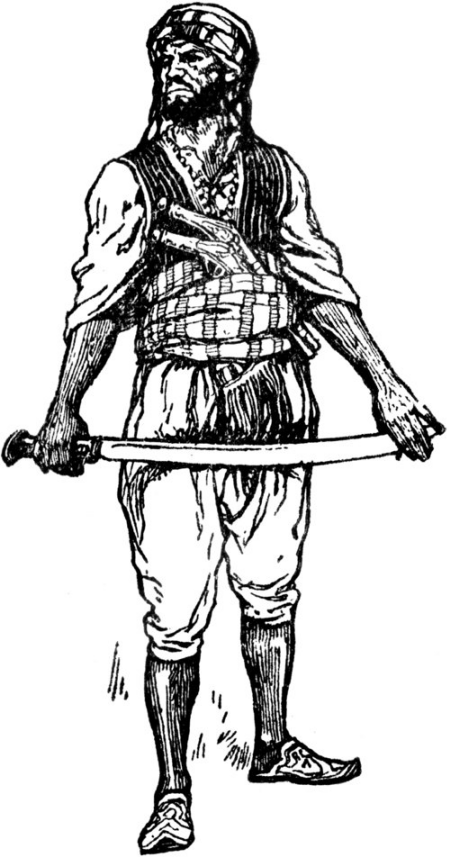
\includegraphics[scale=.3]{Warrior}
  \end{center}


  \myhighlight{Hammerspace}{keyword-hammerspace}
  \flavor {
    "... a fan-envisioned extradimensional, instantly accessible storage area in fiction, which is used to explain how animated, comic, and game characters can produce objects out of thin air." 
  }

  Arcana that make use of Hammerspace allow you to place objects in an "out of game" area until they can be retrieved.  Hammerspace objects can't be stolen, used, or obtained by others - but certain other arcana can tell unsavories whether or not you have things stored in Hammerspace.  You can't put one Hammerspace object in another (they repel like magnets). Objects in Hammerspace immediately return to reality when you die.  No one is really 100\% on how long a living thing can survive in Hammerspace.  

  \myhighlight{Purge}{keyword-purge}
  
  When something is "purged", it removes permanent effects in addition to temporary effects.  For example, the Remedy of \mylink{Bonesetting}{leechcraft-bonesetting} purges a non-serious Physical wound.  




  \newpage

   \mysection{Charms}{arcana-charms}

  You can perform Charms at will.  Casting a Charm takes Moments.  In Combat, invoking a Charm is a Combat Maneuver.

  \begin{center}
  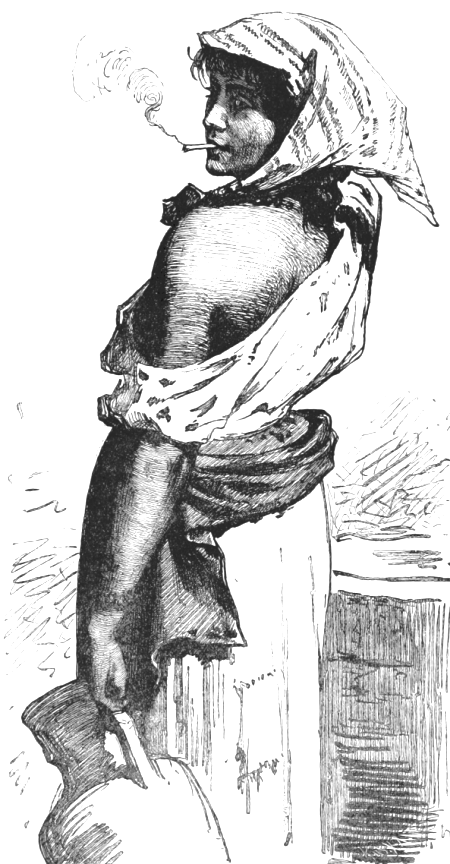
\includegraphics[scale=.5]{Charmer}
  \end{center}


  \cbreak


  \mysubsection{Aphrodite’s Sigh}{charm-aphrodites-sigh}

  By means of this Charm you can create a ghostly moaning sound that appears to come from somewhere Nearby. The moan is not loud nor can it quite cause fear, but any that hear it will know of it's "unnatural" nature. 

  \mysubsection{Candlelight}{charm-candlelight}

  This Charm creates a small mote of light roughly equal to candle light that hovers near your head. The Charm is typically used for reading or lighting a small area (half a cubic meter). This charm cannot be cast into someone's eyes. The light is dim enough that it's not particularly useful for lighting dark passages unless that passage is very well known (such as the your own home). 

  \mysubsection{Creature Comforts}{charm-creature-comforts}

  You can raise or lower the temperature of any non-living material a few degrees, enough to warm or cool food or drinks or a room.  The temperature cannot be raised to a degree where it would injure anyone.


  \mysubsection{Dowsing}{charm-dowsing}

  Using a forked wand of hazelwood, you can sense the direction of a substantial body of potable water.  It ignores "insignificant" amounts of water, as found in a waterskin or barrel.  The Charm doesn’t tell you how hard it might be to get to the water.

  \mysubsection{Fastening}{charm-fastening}

  This Charm allows you to close one door or window that is not locked or otherwise barred. This will not lock the door or window unless by the action of closing it naturally becomes locked. 

  \mysubsection{Flame of Vesta}{charm-flame-of-vesta}

  You may change a fire into one of black flame, so that it casts no light but still provides heat.  You can affect a normal fire up to the size of a campfire.  Furthermore, the flames do not burn, though they are uncomfortable to the touch.

  \mysubsection{Jinx}{charm-jinx}

  You can perform a minor hex by tracing a five pointed star in the air with your forefinger. The hex can affect something Nearby or closer.  These hexes can be severing a rope, shattering a pane of glass, spoiling a piece of food, or some other small act of malice.  Note that these hexes will not work if there is a Pooka nearby

  \mysubsection{Levitate}{charm-levitate}

  You may use this Charm to lift an object via magic alone. The object needs to be non-living and weigh less than 1kg. The object will remain floating in mid-air for up to 1 Hour as long as you are paying at least some attention to it. If you are distracted at all, say in Combat or casting another spell (including another Charm) then the object drops. 

  \mysubsection{Matchstick}{charm-matchstick}

  When you drag your forefinger along a rough surface and says the name of Buer, your fingertip combusts like a giant phosphorus match. It burns for a Moment and does not hurt you in any way.

  \mysubsection{Message}{charm-message}

  You can send a brief message, no more than a dozen words, to a person you know. This person can be any distance away, but they have to be able to understand the language of the message you're sending.

  \mysubsection{Puff of Air}{charm-puff-of-air}

  This Charm creates a small puff of air; enough to blow away dust from objects or to put out a candle, but not enough to put out a torch or lantern. The puff can move very light items as would a puff of air blown from natural means. This charm can be used to blow dirt from an item or area 1m by 1m. 

  \mysubsection{Spice}{charm-spice}

  This Charm flavors one serving of food. The flavor can be changed but it does not change the nature of the food item nor does make poisoned food or spoiled food edible. The flavor can be chosen by you. 

  \mysubsection{Sweet Dreams}{charm-sweet-dreams}

  This Charm allows you to make a willing creature fall asleep. The Charm won't work if used against an unwilling subject. You can cast this Charm on yourself, but this will be the last thing you do that day.

  If used on a subject who is already asleep, you can breathe in their ear and control what dreams they have the following night. No matter how unpleasant the dreams, this cannot prevent the victim from getting a full night’s rest on its own, but it can affect their mood.

  \mysubsection{Third Eye}{charm-third-eye}

  By holding or touching an inanimate object and concentrating for Minutes, you can detect whether or not something is magical in nature, or if something can "hold" an enchantment (including staves, swords, and holy relics).  

  Alternately, you can use this charm to "see" any Nearby concealed objects, like secret doors and hidden compartments.  The Charm doesn't detect invisible or magically concealed objects. 


  \mysubsection{Tidy}{charm-tidy}

  This Charm can be used to clean a single object. The object can be anything: clothing, armor, weapons or even a area of a home. Unlike other Charms this one can be cast on a willing living participant. Casting Tidy on yourself will make you appear as if you had recently bathed and donned fresh clothing. This Charm can clean 1 cubic meter of space or an area 3m x 3m. 

  Alternately, you can fix minor wear and tear in non-living and non-metal apparel as if you were using a needle and thread.  The amount of material mended cannot exceed 1 cubic meter.  You cannot fix a dented piece of armor or sharpen a sword, but you could fix a pane of glass if all the pieces are present, or reattach a broken strap of a backpack

  Finally, you can use this Charm to "freshen" one object up to 1 cubic meter. Typical uses are removing the wrinkles in a garment; brightening the color of some non-living object; making bland food more favorable; or polishing metal or glass. All these effects are considered to be a minor illusion. This Charm can't make poisoned or spoiled food edible. 

  \mysubsection{Turkish Delight}{charm-turkish-delight}

  You can create a single piece of food or drink, such as a Turkish delight, a piece of fruit, or glass of wine. It is exquisitely delicious and provides no nourishment whatsoever. If not eaten within Minutes, it dissolves into black smoke.  You can apply a Toxin to this food if you have one.

  \cbreak

  \mysubsection{Unbolting}{charm-unbolting}

  This Charm allows you to open one door, window, chest or other item that is not locked or otherwise barred. 

  \mysubsection{Watchdog}{charm-watchdog}

  You can place an area of alarm around yourself.  Any creature larger than a cat that comes Close or Nearby to you sets off a mental alarm that will wake you up from non-magical sleep.  You will not know what has entered the circle, but you will know something has, and the the general direction.



  \newpage
   \mysection{The Forgotten}{arcana-forgotten}

\flavor{
  Four Gods wait on the windowsill \\
  Where once eight Gods did war and will, \\
  And if the gods themselves may die, \\
  What does that say for you and I? \Tilde On the Rainslick Precipice of Darkness
}


Three aspects allow you to control the Forgotten:  \mybold{Remembrance}, \mybold{Sovereignty}, and \mybold{Potential}:

\mybullet{
    \item  Remembrance allows you to recall the name of one of the Abandoned, and call them forth from the abyss to do your bidding.
    \item  Sovereignty dictates how many times you can summon one of the Obliterated before you have to rest.  It also governs how many Abandoned you can have summoned at any given time.
    \item  Potential is the power of the Forgotten (Abandoned and Obliterated) under your control
}

The Forgotten will obey you and only you (though some Demons or Abandoned may try to twist your words or intent), but if you are Knocked Out, catch the Vapors, or are otherwise incapacitated, effects may vary (Arbiter's choice) ...

The Forgotten do not speak Acheron - knowledge of their "native" language (Archaic, Seraphic, or Fiendish) is necessary to command them.  You may not summon a creature whose language you cannot speak.  

\cbreak

\mysubsection{The Obliterated}{forgotten-obliterated}

You can summon one of the Obliterated to spy, fight, or distract on your behalf.  You can do this a number of times equal to your Sovereignty before you must rest.  The type of Obliterated you can summon depends on which Anamnesis you know (Beasts, Elements, or Damned).  The Obliterated use your Awareness \UD to Fight and Guard; if they are reduced to 0 Health, or if your Awareness is exhausted, they immediately adjourn. The Obliterated appear as spectral and indeterminate forms; they appears to always be shifting in appearance, and exude a ghostly and ethereal mist or smoke (they clearly do \mybold{not} look normal!)



  \begin{center}
  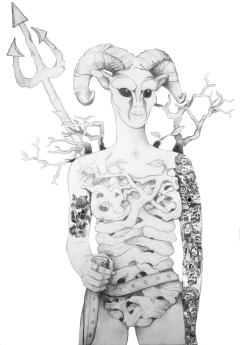
\includegraphics[scale=.5]{Spriggan}
  \end{center}


\myhighlight{Anamnesis of the Beasts}{forgotten-anamnesis-beasts}

Choosing this Virtue allows you to summon a phantom animal to assist you.  The beast will remain under your control for as long as you maintain Concentration, or until Days have elapsed.  This beast can be a mundane sort, or it can be a Zoological Monster (see below).  Beasts only understand \mybold{Archaic}.

\myital{Mundane Beasts:}  The creature will respond to your mental commands, provided they are Close or Nearby to you.  They can follow simple instructions ("get the key on the desk", "chew through these ropes", "spy on that man") but not more complex ones ("pick the lock").  The beast cannot speak. It can be sent on missions a number of kilometers away equal to your Potential. You can see what they see and hear what they hear for as long as you Concentrate. If they take any damage, or if you stop concentrating, they will immediately Adjourn (disappear).

\myital{Monstrous Beasts:}  In addition to animals of a mundane sort, you can also summon a Zoological creature(s) whose combined \HD do not exceed your Potential (if your Potential were 3, for example, you could summon 3 1 \HD beasts, or 1 3 \HD beast, etc).  These creatures will fight on your behalf for as long as you maintain Concentration.  The beasts use your Awareness \UD to Fight and Guard; if they are reduced to 0 Health, or if your Awareness is exhausted, they immediately Adjourn.


\mytable{X c}{
\thead{Beast} & \thead{Potential} \\
}{
    Swarm & * (varies) \\
    Giant Toad & 1 \\
    Troglodyte & 1 \\
    Giant Spider & 2 \\
    Lizard Man & 2 \\
    Giant Lizard & 3 \\
    Dire Wolf & 3 \\
    Giant Ant & 3 \\
    Toad Man & 3 \\
    Giant Centipede & 4 \\
    White Ape & 4 \\
    Giant Snake & 4 \\
    Giant Beetle & 5 \\
    Pteranodon & 5 \\
    Cave Bear & 5 \\
    Salamander & 5 \\
    Triceratops & 6 \\
    Sabertooth Tiger & 6 \\
    Allosaurus & 6 \\
    Plesiosaurus & 7 \\
    Tyrannosaurus Rex & 8 \\
}

\cbreak

\myhighlight{Anamnesis of the Elements}{forgotten-anamnesis-elements}

Choosing this Virtue allows you to parlay with an elemental creature to assist you.  The elemental will remain under your control for as long as you maintain Concentration, or until Hours have elapsed.  This elemental can be a "mundane" sort (an Imp), or it can be a Lesser or Greater Elemental (see below).  Elementals only understand \mybold{Seraphic}.

\myital{Imps:}  The Imp will respond to your mental commands, provided they are Close or Nearby to you.  The Imp is an elemental of a single type (fire, water, smoke, etc) and can take any form you wish, but it can't have a total size in meters greater than your Potential (for instance, if your Potential were 2, it could not be more than 2 meters tall or 2 meters wide). Imps can't cause any damage directly, though they can affect the environment appropriate to its type.  For instance, you could summon a Fire Imp to run into a room to set something alight, or summon a Smoke Imp to stand in a doorway and hide something.   It can follow simple instructions ("jump into the hay (Fire)", "douse the fire (Water)", "blow out the torches (Air)") but not more complex ones ("burn the book the lich is carrying").  The Imp cannot speak. The Imp can't move further than Far Away from you.  Unlike Beasts, you cannot see what they see or hear what they hear (they make terrible spies). If they take any damage, or if you stop concentrating, they will immediately Adjourn (disappear).

\myital{Elementals}:  In addition to Imps, you can also summon Lesser or Greater elementals whose combined \HD do not exceed your Potential.  The elemental will fight on your behalf for as long as you maintain Concentration.  The elementals use your Awareness \UD to Fight and Guard; if they are reduced to 0 Health, or if your Awareness is exhausted, they immediately Adjourn.


\mytable{X c}{
\thead{Elemental} & \thead{Potential} \\
}{
    Lesser & 5 \\
    Greater & 7 \\
}

\newpage

\myhighlight{Anamnesis of the Damned}{forgotten-anamnesis-damned}

Choosing this Virtue allows you to wrest a Demon from the depths of Hell to obey you.  The Demon will remain under your control for as long as you maintain Concentration, or until Minutes have elapsed.  This Demon can be a "mundane" sort (a Gremlin), or it can be a Demonic monster (see below).  Demons only understand \mybold{Fiendish}.
All Demons are Unhallowed. 


\myital{Gremlins:}  Gremlins can be summoned somewhere Close or Nearby to  you.  Gremlins can only cause havoc and chaos; you can partially guide them, but generally they are under the control of the Arbiter.  When they are summoned they immediately run in different directions (but won't move further than Far-Away from you) and cause as many problems as they possibly can - unbuckle belts, set things on fire, cut ropes, smash pottery, scream and kick in the middle of the floor, etc.  They may or may not follow instructions (Arbiter's discretion.  If you're stuck, roll a die and have them react randomly).  You can see what they see and hear what they hear, but it's generally unpleasant to do so.  You summon a number of Gremlins equal to your Potential.  If they take any damage, or if you stop concentrating, they will immediately Adjourn (disappear).

\myital{Devils:}  In addition to Gremlins, you can summon various types of Devils whose combined \HD do not exceed your Potential (if your Potential were 3, for example, you could summon 3 1 \HD Dretch, or 1 3 \HD Vrock, etc).  These Devils take no damage from iron weapons or from spells \mybold{not}  of the Entropy paradigm. Seeing a Devil prompts a Sanity check (including for Allies!).  See the Bestiary for further information on Demons.

\mytable{X c}{
\thead{Demon} & \thead{Potential} \\
}{
    Dretch & 1 \\
    Vrock & 3 \\
    Slaad & 5 \\
    Naga & 7 \\
    Balor & 9 \\
}

\cbreak

\mysubsection{The Abandoned}{forgotten-abandoned}

In order to summon the Abandoned, you call them forth using their True Name - represented by your Remembrance.  Remembrance is either bound or unbound.  You can use an unbound Remembrance to recall the name of \myital{any} Abandoned (essentially, tell the Arbiter the name of the Abandoned you wish to call forth when you're ready to summon them).  From then on, that point of Remembrance is now bound to that Abandoned, and you can only use it to summon that specific Abandoned. You can add additional unbound Remembrance points when you gain levels; alternately, the Arbiter may place the True Names of various Abandoned as treasure in the game.  Learning the True Name of one of the Abandoned from treasure in this way counts as a "bound" Remembrance.

Any attacks against the Abandoned automatically succeed.  They can take up to your Potential x 5 points of damage before they Adjourn (so if you had 3 Potential, they would be able to take 15 points of damage).  If an Abandoned adjourns for any reason during a Session, it will not return until the next Session. You can have a number of Abandoned summoned equal to your Sovereignty at any time, but be warned - Abandoned are fickle and proud spirits, and may not cooperate with other Abandoned.

Unless otherwise noted, Abandoned will not Adjourn until the end of the Session unless they can be somehow convinced to do so (or if they take enough damage to force them to Adjourn).  The Abandoned have memory and personalities, and won't take kindly to being forced to Adjourn by "killing" them!

Below are the 12 Archons, Seraphs, and Fiends who can be summoned via their true name.  This is by no means a complete list - feel free to work with an Arbiter to create different Abandoned.  Archons speak Archaic; Seraphs speak Seraphic; and Fiends speak Fiendish.


\newpage

\ed{Lots of influence from Skerple's mind-blowing \href{https://coinsandscrolls.blogspot.com/2019/10/osr-glog-based-homebrew-v2-many-rats-on.html}{GLOG Homebrew v.2}}



\mysubsection{The Archons}{forgotten-archons}


\myhighlight{Big Mac, "Good Time Guy"}{abandoned-big-mac-good-time-guy}

Big Mac crashes through a window or door and drunkenly hugs the first person he sees. He appears as a portly robed monk with a tankard of beer and a rosy complexion.  He is totally smashed and very happy.  

Unless Big Mac is at a party (at minimum, drinks and 2 happy people) he will leave the way he came in with an "Irish goodbye" (adjourning).  If there's a party, he will continue to drink from his tankard (which never gets empty), tell tall tales, reminisce, propose mad schemes, sing songs in all languages, provide terrible advice, and sometimes throw up.  He cheers up any low-class social event and scandalizes anyone tasteful. Big Mac can find a number of items equal to your Potential for you, provided they are party related.  Examples:  more beer, a safe place to crash, a person of negotiable virtue, Pooka, narcotics, musicians.  He can remove Toxins or Drunkenness from a number of people equal to your Potential.

\myhighlight{Bon Chapeau, Hat of Marvels}{abandoned-bon-chapeau-hat-of-marvels}

Bon Chapeau enters with a burst of light on a target's head up to a distance of Far Away.  It appears a magnificent hat, crown, turban, etc. depending on how Bon Chapeau is feeling that day (but it will always match the wearer's garments).  

If the wearer is under the effect of a Mind spell when the hat appears on their head, the spell is immediately broken.  If someone attempts to cast a Mind spell against the wearer, the spell rebounds on the caster. 

The hat can hear the wearer's thoughts, and will tell them to you if asked.  It can also judge fashion shows and tell you if an article of clothing is a knock off or not.

\myhighlight{Bufo, the Lickable Toad}{abandoned-bufo-the-lickable-toad}

A fat green toad the size of a housecat hops in.  He has yellow eyes and many warts, and speaks in a booming croak. 

Anyone who licks Bufo must make a Sanity check; if they succeed, they can invoke one of the following effects:
\mylist {
\item they can restore all Intangible Stats to their \MAX
\item they can heal their Flesh fully, or
\item they can heal their Grit fully
}

Bufo doesn't like being licked.  There is a cumulative 1 in 6 chance that anyone who that licks him will gain no positive effect (i.,e.  on the second lick, there is a 2-in-6 chance it will have no positive effect, a 3rd 3-in-6, etc).  Once this number hits 6-in-6, no further beneficial effects can occur for the remainder of the Session.

Objects swallowed by Bufo enter Hammerspace until he adjourns, when he will spit them back out.  He'll only swallow things that look delicious (but he's easily tricked).  The object swallowed can't be bigger than he is.



\myhighlight{Gemma, Translator of Mysteries}{abandoned-gemma-translator-of-mysteries}

A thin, tired woman with wiry hair appears wherever you're not looking.  Gemma can speak and translate any language (living or dead), and will translate for you in real time.  Gemma won't speak or translate blasphemies (which are basically things written in Fiendish or Seraph).  If Gemma is reading by the light of the sun, she'll prepare a full allegorical and contextual translation.  She can't (or refuses to) write.  While Gemma is Close to you, you can't be Befuddled (and ends any Befuddled effect on you if applicable).

\myhighlight{István, the Lost}{abandoned-istván-the-lost}

A tired, middle-aged man with blue eyes shuffles in politely.  Anyone who talks to István will give him directions to any place you name.  Directions given will be to the best of the person's knowledge, and can include the location of treasure, traps, hazards, patrols, etc. etc.  Ask a peasant how to get to the moon and he'll shrug and suggest a mountain; ask the Grand Archmage of the Isle of Carcosa and you might get a very different answer.  


\myhighlight{Judyth, the Tiebreaker}{abandoned-judyth-the-tiebreaker}

Judyth is a floating stone sphere about bowling ball sized, carved in the shape of a human head.  She floats down from the ceiling and speaks with a decisive, stern voice.  If two objects, items, ideas, or issues are presented to Judyth (along with some criteria for judging) she will judge their merits. For example, you could ask "Which of these gems is most valuable?", "Which of my friends loves me most?" or "Which of these two mushrooms is tastes better?" Judyth can't answer questions that aren't local and immediate:  "Which country will win the war?" or "Which hallway did the thief run down?" aren't allowed, for example.  If Judyth is presented with a paradox, she will immediately adjourn in a logic bomb that deals your Potential x 3 damage to everyone Close (Save for half).

\myhighlight{Mikhael, the Justifier}{abandoned-mikhael-the-justifier}

A middle-aged, completely bland man enters with a shuffle.  You can't really describe him further than that; his appearance seems to be easily forgotten.  In a low and soothing voice. Mikhael will assist anyone in justifying any plan (or crime).  People who talk to Mikhael are freed of any guilt or doubt.  Mikhael has no secret knowledge, but hints vaguely at schemes by people in power (kings, religious leaders, etc).  

Any arrows or projectiles aimed at Mikhael or anyone Close to him automatically miss (whether they are Allies or Monsters)


\myhighlight{Mon Signor, the Deliverer}{abandoned-mon-signor-the-deliverer}

A bellboy comes running in with a patter of feet.  He hands you a package that contains d6 \UD of Provisions, waits for a tip (doesn't always get one), and then runs off - immediately adjourning.  The Provisions are always weird - a little too warm, a little too salty, a little too spicy, etc.  You can hand Mon Signor any item and it will be returned to you the next time he is summoned as if no time has passed (this item exists outside of Hammerspace, and can be the size of a human body)

\myhighlight{Randy.  Just Randy}{abandoned-randy-just-randy}

A pop, a short scream, and Randy falls down from the ceiling.  He is an acned teenage human with brown hair and a torn blue robe.  Randy was once a wizard's apprentice; a botched spell trapped him in a pocket dimension where he lives on, immortal and extremely confused. He is perpetually being dragged into combat, danger, dismemberment, and extremely awkward situations. 

Randy will sort-of obey you for the Session, but he is only an immortal teenager. He's awful at everything. If you want, you can direct any physical attack against you to Randy instead.  If you have more than 3 Potential, Randy's efforts are accompanied by appropriately dismal music.  Randy insists on an honorific i.e. "Randy the Magnificent", "Randy the Stupendous", etc. but no one ever calls him that.

\myhighlight{Smök, the Grey Messenger}{abandoned-smök-the-grey-messenger}

Smök seeps in through cracks in the floor and ceiling, appearing as a grey flag flapping in the wind.  You can give Smök a message containing a number of words up to your Potential or an object smaller than an apple - the apple or message will vanish, and Smök will move as quickly as an arrow (325km/h), to bring the item to location or person you designate.  If Smök can't reach the target by the end of the Session, it will drop the item somewhere along the quickest path.


\myhighlight{VVulf, Trapfinder}{abandoned-vvulf-trapfinder}

The sound of a trap springing shut echoes through the room, and a starving 3-legged wolf appears before you, fur matted with blood.  VVulf can detect any traps Nearby until he adjourns.  Zoological animals feel affinity with VVulf - provided combat has not been initiated, the Monster will not attack if they fail a Morale check.  VVulf is able to talk to mundane animals and ask simple questions (and receive basic answers).  VVulf immediately adjourns if anyone Nearby exhibits cruelty towards an animal.

\myhighlight{Weeble, the Wobbling Stone}{abandoned-weeble-the-wobbling-stone}

A stone egg of a rotund, happy man with a cheerful grin appears in your hand.Anyone holding Weeble cannot be knocked Prone or Stunned.  If you would fall into a pit or off a cliff, Weeble wobbles you back to safety at the last possible moment - but Weeble can't help you if the bridge collapses or your boat explodes or what-have-you.  If you had Weeble to any liquid (soup, wine, etc) it will neutralize any Toxins inside.



\mysubsection{The Fiends}{forgotten-fiends}


\myhighlight{Al Ana, the Slaughtercaller}{abandoned-al-ana-the-slaughtercaller}

A red stone carved with a snarling tiger biting its own tail appears with a sizzle in your hand.  All weapon damage dealt within a Close or Nearby radius of Al Ana is doubled (from Allies and Monsters).  If you throw Al Ana using your \DEX, it will deal your Potential in damage (i.e. if your Potential is 4, it will deal 4 damage on a successful hit) and return to your hand at the bottom of the Moment.  Al Ana growls before ambushes, making you immune to Surprise.

\myhighlight{Ben Sidhe, Singer of Death}{abandoned-ben-sidhe-singer-of-death}

A spectral woman with long, streaming hair boils up from the floor in a white mist.  She wears a grey cloak over a green dress, and her eyes are red from weeping.  She immediately begins wailing.  All creatures Nearby (except you) take your Potential in damage.  The damage increases by +1 and repeats at the top of each Moment after the first until a Save vs. Doom is made.  Ben Sidhe cannot be silenced and will not stop weeping until she adjourns.  She will always remain Close to you.

\myhighlight{Diviseré, the Universal Chisel}{abandoned-diviseré-the-universal-chisel}

A simple iron chisel with a wooden handle appears in your hand.  Diviseré can separate any two layers.  You could separate skin from muscle, gold foil from wood, rust from iron, or the bark from a tree. You can't separate things that are not fused, so Diviseré couldn't chisel the armor off a warrior or the nose off a statue (at least, not any more than a normal chisel could). Diviseré can separate things joined by Brahe's Efficacious Sealant.  Diviseré can't speak


  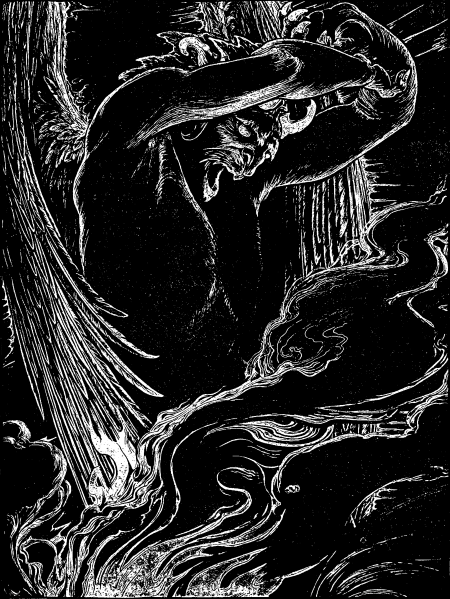
\includegraphics[scale=.45]{Demon}

\myhighlight{Doppel, the Mirror}{abandoned-doppel-the-mirror}

An identical duplicate (save for some subtle detail, like a different eye color) of you steps from your shadow.  Doppel will act as directed by you, including very complex tasks (though Doppel can't improvise).  Doppel can't deal damage or cast spells, but can invoke minor Illusions to make it appear that it can.  Doppel is unable to speak.

\myhighlight{Gitgud, the Taunter}{abandoned-gitgud-the-taunter}

A skinny monkey in torn robes appears with a low whistle.  Gitgud has a toothy, sneering grin and tiny red eyes.  Gitgud will taunt any target you tell it to with capers, jeers, wails, and jokes.  He is really distracting and annoying.  The target must Save vs Doom or immediately attack Gitgud, who will run away to taunt from a safe distance.  He can climb and perform simple tasks with a monkey's patience and skill.

\myhighlight{Grendel, the Helping Hand}{abandoned-grendel-the-helping-hand}

A blue-green arm and hand drops from the sky with a wet thud.  The arm can be stuck to flesh and acts as an extra limb.  On a willing target, Grendel grants an additional Unarmed attack each Moment that deals your Potential in damage (\MAX 6).  Use the target's \FOC instead of \VIG or \DEX when they make their Fight roll.  It can carry a shield or a lantern, or assist with climbing or swimming (+2 to the roll), but cannot wield a weapon.  If attached to an unwilling creature, Grendel will punch them in the nearest vulnerable spot, deals your Potential in damage (\MAX 6).  The arm detaches with a pop;  it can be stuck to a number of creatures equal to your Potential every Session.

\myhighlight{Grimalkin, Ruler of the Weak}{abandoned-grimalkin-ruler-of-the-weak}

A purring grey cat with yellow eyes comes curling out from the shadows between your legs.  Grimalkin is an asshole; she'll ignore what your asking her, get into trouble, and generally be a nuisance.  However, she can also do the following:

\mylist {
    \item Eat a Curse (see \mylink{Hekaphage}{occultism-hekaphage});
    \item Turn any die roll that hits the table into a natural 1;
    \item Knock a single die off the (real world) table. The roller gets a re-roll.
}

She can perform any of those abilities a number of times equal to your Potential, at which point she adjourns.

\myhighlight{Lucertola, the Taster}{abandoned-lucertola-the-taster}

A sleek yellow lizard with a bright blue tongue appears around your neck.  Lucertola can taste the air and tell you about the source of odors, smoke, fog, etc.  If you give Lucertola a taste of food or drink, it can tell you whether or not its safe to eat or drink.  While you're wearing Lucertola you can breathe underwater, and you're immune to inhaled Toxins.

\myhighlight{Mirót, the Critic}{abandoned-mirót-the-critic}

A tinkling of glasses and a cleared throat herald a balding man in a tweed jacket, or woman of impeccable dress and haughty expression, who step out from a nearby doorway.  In either form, Mirót's eyes are milky white.  Mirót hates all works of art, and will move from room to room, destroying any artwork, carvings, decorations, or written works it can see (Grimoires and Fetishes not included).  This also includes objects that can create art - instruments, paints, paintbrushes, inks, and empty scrolls and papyri.  It won't ever attack a living creature, but can set things on fire with a touch.  Mirót is a blunt instrument - if prevented from entering a museum, for instance, it will burn the museum to the ground in order to destroy the art inside.  If an actual artist is present (musician, painter, sculptor, writer, scribe, etc) Mirót will hurl insults and epithet's at the artist in a non-ending stream of vitriol; all \RO and \RS attempts by the "victim" are at -4 as long as he or she is forced to endure the onslaught.  Mirót will adjourn if there is nothing around it to criticize, and nowhere else for it to go.


\myhighlight{Nyumbu, the Broken}{abandoned-nyumbu-the-broken}

A broken, skeletal mule with fire burning in its eye-sockets clatters in from behind you.  Nyumbu can carry up to 50 Significant Items for you and can travel over water and air as if it were solid ground.  It can only walk in a straight line and can't jump - you could lead Nyumbu up to a cliff face and over a chasm, but unless there were a cliff of equal height on the other side, it will remain hovering in air.  As long as your hand is on Nyumbu's bridle, it conveys the ability to walk on water and air to you as well.  When Nyumbu adjourns, everything it was carrying falls on the ground.  If Nyumbu is ever struck for damage by someone Close, it will immediately kick at the attacker and automatically deal damage equal to your Potential; regardless of the range of the striker, Nyumbu will immediately adjourn if struck, dropping what it was carrying (and potentially yourself) onto the ground.

\myhighlight{Orobas, the Moneychanger}{abandoned-orobas-the-moneychanger}

A squashed and twisted homonculous with a huge gut and tiny limbs appears in a puff of cigar smoke.  Orobas sports a top hat, monocle, and cigar but has not neck or eyes to speak of.  Orobas will eat any coins you give to it, and spit them back up at your request at any point (even if summoned years later).  These coins exist outside of Hammerspace.  Orobas will only eat Iron, Silver, or Gold coins - not jewelry, gems, or anything else.  Orobas can accurately state the amount of money a person is carrying at any given time, or the number of coins (and types) in a pile.  He can give you "business advice", but it almost always involves killing someone.


\myhighlight{Pocong, the Piper}{abandoned-pocong-the-piper}

A tiny grey cloth effigy of you with strange, wet-looking eyes appears in a glimmer of light.  As long as Pocong is Close to you, you automatically pass any Saves vs Doom.  Pocong can't move on its own.  If the effigy is moved away from you to somewhere Nearby, or adjourns by taking damage, you must Save vs. Doom (not automatic!) or immediately be brought to 0 Flesh, prompting a \DEATH roll.



\mysubsection{The Seraphim}{forgotten-seraphim}


\myhighlight{Ada, the Calculator}{abandoned-ada-the-calculator}

A young woman with black hair and expensive Victorian garb appears from somewhere behind you.  Ada can measure the exact distance between two points (provided one of them is within sight) and immediately know the direction of true north no matter where she is.  She can rapidly calculate any number of items provided they are separated from one another (she couldn't count the number of coins in a pile, for instance, unless that pile was separated into individual coins).  As long as Ada remains Close to you, you automatically succeed on all Skill:Math checks.



\myhighlight{Beatrix, the Story Teller}{abandoned-beatrix-the-story-teller}

A very old woman in clean Victorian clothes enters with a polite knock and a quiet shuffle.  She carries an empty scabbard and a book tucked into an apron pocket.  If a fight breaks out with Beatrix present, she summons a rocking chair, pulls out the book, sits, and begins reading in a sweet and mesmerizing voice understood by all present.  Allies and Monsters alike must Save vs Doom at the top of each Moment or fall under the sway of Beatrix.  They will sheathe their weapons, sit at her feet, and listen to her story.

\myhighlight{Bíró, the Chronicler}{abandoned-bíró-the-chronicler}

A black quill of an unknown beast, half a meter in length, appears in your hand.  Bíró can't speak or see, but can hear excellently.  If you provide it ink (the blacker the better), Bíró will write the answers to any questions you ask as long as its heard the answer in the time since you summoned it.  It can transcribe conversations in perfect detail or tell you how many people entered a room, what they said, and when they left.

If anyone holds Bíró against your will, they must Save vs.  Doom or be reduced to 0 Health / Flesh.  If anyone holds Bíró with your permission, they must Save vs. Doom or become Charmed to you for Hours.  Either way,  Bíró adjourns if anyone other than you holds it.

\myhighlight{Crescendo, Choir of Heroes}{abandoned-crescendo-choir-of-heroes}

A quickly rotating cube appears above you, sending out rays of electric light with illumination as a torch, and begins chanting.  The chant fills the hearts of Allies with hope, courage, and the belief that if they can just see things through, everything will be OK.

Every Ally Close or Nearby to Crescendo is immune to Fear and anything that might cause despair (like the Wall of Gloom). If invoked during Combat,  Allied Hirelings all gain fanatic morale, and Allies regain your Potential in Grit at the top of each Moment (if they are at 0 Flesh, they still must roll their \DEATH however).  The Crescendo will adjourn at the end of your next Combat (or unless you tell them too).  

\myhighlight{Flux, the Hallowed Light}{abandoned-flux-the-hallowed-light}

A sphere of golden flame appears in a shimmer of light, shedding light as a torch.  Flux can flare and illuminate (briefly) an area from Close to Far-Away.  Sighted creatures in the area who aren't prepared must Save vs Doom or be Blinded for d4 Markovian.  The flare can even temporarily cancel magical darkness; it will re-emerge at 5m per Moment from its source.  Unhallowed won't approach Flux unless forced.

\myhighlight{Leroy, the Lucky Rose}{abandoned-leroy-the-lucky-rose}

A red rose with a silver stem appears in your hand.  Leroy inspires foolish confidence in anyone who wears him as a boutonnière.  The wearer will accept any risky but thrilling plan they are presented with. Provided the endeavor is risky enough (Arbiter's discretion), the wearer will receive +4 on all \RO or \RB attempts in pursuit of the plan.

\myhighlight{Pferdinana, the Sure Bet}{abandoned-pferdinana-the-sure-bet}

An ordinary-looking but tidily brushed grey mare appears with a clatter of hooves.  Pferdinana can speak to horses, but translates with snide remarks and uncomfortable, mocking laughter.  Pferdinana will permit you to ride her, but travels at a slow trot, sighing with boredom.  However, if she's asked to race another creature, she will win any race over any terrain, no matter how terrifying or improbable.  If your Potential is 5 or greater, Perfidnana will race inanimate objects, spells, the weather, etc.

\myhighlight{Sir Ector de Mares, First of the Snail Knights}{abandoned-sir-ector-de-mares-first-of-the-snail-knights}

A stooped man in a visored helmet, wearing antique armor, enters in through a door or window.  He creaks when he walks.  If called upon as a second in a duel, Sir Ector grants the following powers:

\mylist{
\item The duelist wins Init every Moment; 
\item The duelist cannot be disarmed; and 
\item The duelist gains +4 on all Fight and Guard rolls.
}

Sir Ector can tell true kings from false ones at a glance.


\myhighlight{Termagant, "My Old Lady"}{abandoned-termagant-my-old-lady}

When remembering Termagant, select a number of Hours from now when she should show up (immediately is fine).  At the designated time, a middle-aged woman of suitable race and appearance for the area enters screaming general accusations ("Coward!  Bastard!  Bitch!  etc.")  She grabs you and drags you away.  Termagant's appearance might be enough to convince guards or authority figures not to stop her, but if that fails she produces false documents, bribes, "proof", etc. - whatever it takes to get you out of the situation you're in short of violence.  She drags you out of sight and then promptly adjourns.  She'll only rescue you (not anyone else), and won't return for anything you left behind.  She can't heal you.  No barriers (magical or no) can hinder her, but she'll only take you to the next unlocked and unobserved area, then adjourn.

\myhighlight{Trismegistus, the Herald's Wand}{abandoned-trismegistus-the-heralds-wand}

Trismegistus appears in a stream of leaves and smoke as a shillelagh with a snake wrapped around it.  It will remove any a number of Diseases equal to your Potential.  Once it's reached its limit, it will hop along next to you and get into trouble.  Trismegistus can translate for any reptiles you might come across.

\myhighlight{Veritas, the Truth Teller}{abandoned-veritas-the-truth-teller}

An old man in fine robes or a beautiful young woman with no hair enters from somewhere behind you.  Veritas mutters like a madman, repeating meaningless phrases, snippets of conversation, and rocking back and forth.  As long as Veritas can see the tongue of a creature, it can tell if the creature is lying; if it detects a lie, it will lunge at them and remove their tongue.  The tongue stays in a pouch on its belt until it adjourns (at which point it returns to the tongueless victim with no ill effects).  Veritas can carry up to 25 Significant Items for you and will provide banal and useless advice if asked.


\myhighlight{Walden, the Quartermaster}{abandoned-walden-the-quartermaster}

A portly man with grey eyes and stained clothes enters from somewhere behind you.  You can ask Walden for up a number of items up to your Potential, and he will procure them for you.  The items must be mundane in nature and can't be specific:  "a pair of woolen trousers" or "a longsword" are OK, but "the cape of Felspex the Witch", "the magical blade of Aesop", or "a Grimoire containing the following spells" aren't possible.  If the item has a \UD attached (a quiver of arrows, for example) Walden will provide d4 \UD of the item (this means he can provide Heavy armor, but it only has d4 \UD, for instance).  If Walden adjourns, the items disappear.  Walden can identify who forged any weapon shown to him; when it was forged; and when the weapon was last used.







  \newpage
      \newpage

    \mysection{Leechcraft}{arcana-leechcraft}


  \example {
    \mybold{Knowledge Die} + Modifiers vs. Target
  }


    The art of Leechcraft allows you to practice \mybold{Remedies} by rolling your Knowledge Die vs. a Target (see below).  Unless otherwise noted, Leechcraft requires 2 Actions to perform.  The recipient of the Leechcraft \mybold{cannot move} while you are applying your medicines.  Your \INT adds a bonus to your roll:

    \mytable{X r}{
      \thead{\INT} & \thead{Bonus} \\
    }{
      d2-d10 & +0  \\
      d12 & +1  \\
      d16 & +2  \\
      d20 & +3  \\
      d24 & +4 \\
    }
   
  If you roll less than the Target number, your next roll is at -2.  This is cumulative:  -2 for the first miss, -4 for the second, etc.  These negatives are removed when you take a \mylink{Bivouac}{combat-resting-bivouac}. When rolling, your \SUMDICE can never be less than 1.

  


  


  \LEECHCRAFT[
    Name=Bonesetting,
    Link=leechcraft-bonesetting,
    Target=9,
    Keywords=Purge,
    Reversible=Y
  ]

  Can only be performed during a Bivouac.  Purge a single non-serious Physical Wound.  If desired, you can use this 'craft to cause a non-serious Physical wound (your choice).  

  \LEECHCRAFT[
    Name=Delay Infection,
    Link=leechcraft-delay-infection,
    Target=7,
    Keywords=None,
    Reversible=Y 
  ]
  
  Can only be performed during a Breather or Bivouac.  Delay the onset of a single Disease (including contagion) for the rest of the Session.  If desired, you can use this 'craft to speed the disease along (Arbiter's discretion - the disease should move 1 "step" in a worse direction).

  Curing Disease requires \mylink{Medicinals}{research-medicinals}

  \begin{center}
  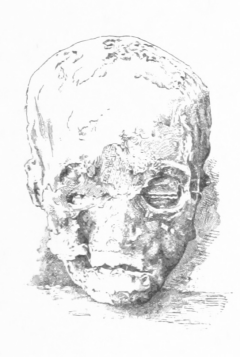
\includegraphics[scale=.5]{Skull}
  \end{center}


  \LEECHCRAFT[
    Name=Hair of the Dog,
    Link=leechcraft-hair-of-the-dog,
    Target=2,
    Keywords=Purge,
    Reversible=N
  ]

  Purge the effect of a Hang Over on a single person.

  \LEECHCRAFT[
    Name=Laudanum,
    Link=leechcraft-laudanum,
    Target=9,
    Keywords=Purge,
    Reversible=Y 
  ]

  Remove a Disgusted, Shaken, or Sickened effect on a single patient.  If applied during a Bivouac, Purge a single non-serious Mental Wound.   If desired, you can use this 'craft to cause a non-serious Mental wound (your choice) during a Bivouac.

  \LEECHCRAFT[
    Name=Mend,
    Link=leechcraft-mend,
    Target=2,
    Keywords=None,
    Reversible=Y
  ]

  Can only be applied to a patient who is Dying. Heal 1 Flesh.  

  You can also use Mend to cause a point of damage to a dying person (prompting a \DEATH roll).  The attempt isn't noticeable to others unless they're practiced in Leechcraft.

  \LEECHCRAFT[
    Name=Purge Toxin,
    Link=leechcraft-purge-toxin,
    Target=6,
    Keywords=None,
    Reversible=N 
  ]

  Immediately purge a Toxin from the body of a single patient

  \LEECHCRAFT[
    Name=Restore Senses,
    Link=leechcraft-restore-senses,
    Target=6,
    Keywords=None,
    Reversible=N 
  ]
  Remove a Blindness or Deafness effect on a single patient

  \LEECHCRAFT[
    Name=Sew Wounds,
    Link=leechcraft-sew-wounds,
    Target=4,
    Keywords=None,
    Reversible=N
  ]
  You can only perform this during a Breather or Bivouac. The patient rolls 1 \FLESH and heals that much Flesh.

  \LEECHCRAFT[
    Name=Smelling Salts,
    Link=leechcraft-smelling-salts,
    Target=3,
    Keywords=Purge,
    Reversible=N
  ]
  Purge a Knocked Out effect on a single patient


  \LEECHCRAFT[
    Name=Staunch,
    Link=leechcraft-staunch,
    Target=4,
    Keywords=Purge,
    Reversible=Y
  ]
  Purge or cause a Bleed effect on a single patient


  \LEECHCRAFT[
    Name=Trepanation,
    Link=leechcraft-trepanation,
    Target=8,
    Keywords=Purge,
    Reversible=Y  
  ]
  You can only drill holes in peoples' heads during a Bivouac.  Purge a Woozy effect on a single patient.   If desired, you can use this 'craft to cause the patient to become Woozy instead.

  \LEECHCRAFT[
    Name=Virtigo,
    Link=leechcraft-virtigo,
    Target=6,
    Keywords=None,
    Reversible=Y 
  ]
  
  Bivouac only.  Purge a Befuddled or Concussed effect on a single patient.   If desired, you can use this 'craft to cause the patient to become Befuddled or Concussed



  \newpage
  % (c) 2020 Stefan Antonowicz
% Based off of tex found at https://github.com/ludus-leonis/nipajin
% This file is released under Creative Commons
% Attribution-NonCommercial-ShareAlike 4.0 International License.
% Please do not apply other licenses one-way.

\mysection{Liturgies}{arcana-liturgies}

The core Liturgies of the Ten Authorities can be found below.  Your personal Faith in a Small God allows you to invoke the Liturgies of the Authority they sit beneath. During your adventures, you may also find Liturgies of your Small God etched on bronze tablets hidden by fearful priests in stinking swamps, forgotten in reliquaries lying in pawn shops, or written in the slime of snails tripping balls on shrooms (Liturgies of your Small God depend completely on the Arbiter)

\mybold{Liturgies require a Holy Symbol to perform}.  If you don't have your Holy Symbol, you get none of the benefits of a Liturgy, and you can't invoke any of the powers beneath it.




\mysubsection{The Contract}{liturgies-the-contract}

The Small Gods must obey certain "rules" when dealing with Mortals:

\mynumlist {
  \item  The Small Gods must be true to their nature
  \item  The Small Gods must hear what Mortals have to say, and they must honor their bargains
  \item  The Small Gods can only hear a Mortal's words - they cannot hear their thoughts
  \item  The Small Gods must speak truth to Mortals about what is happening in distant places
  \item  The Small Gods must prophesy honestly - though they may try to trick Mortals with their words
}

\mysubsection{The Holy Symbol}{liturgies-holy-symbol}

Your Holy Symbol allows you to harness your Faith to perform the Liturgies of your Small God.  Tell the Arbiter what the Holy Symbol of your Small God is (there are some ideas under the section on \mylink{Authorities}{mystics-authorities} below)

A Holy Symbol is a \mylink{Holy Relic}{miracle-holy-relic}; you must perform the Miracle of \mylink{Holy Relic}{miracle-holy-relic} to create a new one if yours is lost or destroyed.  Remember that your Holy Symbol contains a single Faith die that you can use in a pinch.  If you use this Faith Die and roll a Failure, the Faith Die is lost and the Holy Symbol becomes a normal item (and can't be used to perform Liturgies)

You don't need a Holy Symbol to practice the \mylink{The Seven Sacraments}{arcana-seven-sacraments}

  \begin{center}
  
\includegraphics[scale=.5]{Mystic_2}
  \end{center}



\newpage

  \begin{center}
  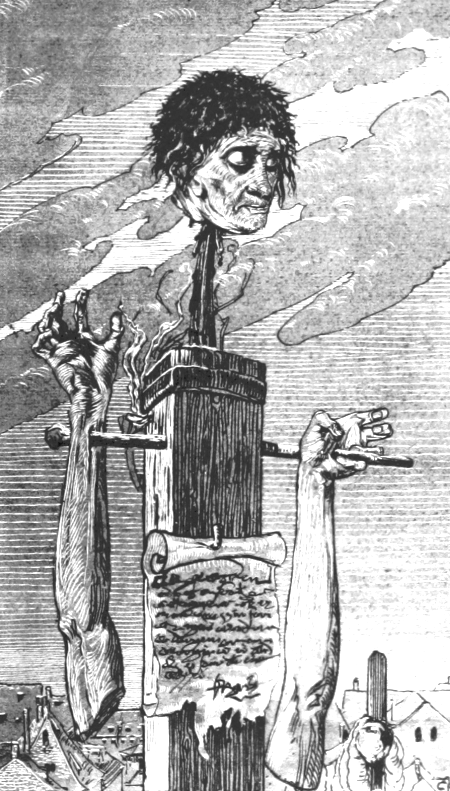
\includegraphics[scale=.5]{Crucifixion}
  \end{center}


\mysubsection{Divine Favor}{liturgies-divine-favor}

You may call upon your Small God to directly intercede on your behalf.  To do this, you must roll \mybold{all} of your Faith dice, the \SUMDICE of the roll must be 60 or better.

The divine favor must be something your Small God would have some control over, based on their aspect (Arbiter's discretion).  For example, Vulcan (Small God of fires, volcanoes, and the forge, who sits beneath the Civilized Authority) might not be able to affect the curse of the Ice Queen.  

The Small Gods cannot violate the basic laws of the Authority:


\mybullet {
  \item Matter and energy can neither be created nor destroyed, as this is the demesne of \TheAuthority; they can only be transformed or changed from one form to another.  Once a spirit has departed for the Isle of the Dead, it is beyond the reach of the Small Gods forever. 

  \item Entropy always increases.  Time cannot flow backward; sword strikes cannot heal; you cannot "fall" against the direction of gravity. It is possible to suspend this Law (to roll back time, for instance), but only for a few Moments before it reverts to entropy again.

  \item A \myital{noumenon} cannot be removed by a Small God. A Small God cannot directly slay something on the Mortal plane.

  \item All matter and energy has a destiny in the dream of \TheAuthority.  A Small God cannot cause matter or energy to do something that violates this destiny, and the ultimate destiny is only known to \TheAuthority. (Practically, this means the effects of a Divine Favor are up to the Arbiter's discretion in the end!)

}


The Small God may also demand a sacrifice of some kind, or expect payment later ...


\example {
  \mylist {
    \item Time rolls back for a few seconds to stop a killing blow from falling, or to re-roll a missed Save.

    \item A powerful magical item or artifact needs to be sundered

    \item A sea must be parted, a tunnel opened through a mountain, or a boulder pushed to seal an entrance

    \item Stones and trees, or sand and ice, assemble themselves into a fortress to protect the faithful
  }
}




\newpage

\mysubsection{The Authorities}{mystics-authorities}

The Small Gods sit in uncountable multitudes beneath the ten Authorities (though there are said to be 13 in all, 3 hidden from the eyes of Mortals). Your personal Faith in a Small God allows you to invoke the Liturgies of the Authority they sit beneath. Each Authority has four core Liturgies practiced by the faithful: 

\mybullet {
    \item the Liturgy of the Novitiates;
    \item the Liturgy of the Clerics;
    \item the Liturgy of the Apostles; and 
    \item the Liturgy of the Saints
}


During your adventures, you may also find Liturgies of your Small God etched on bronze tablets hidden by fearful priests in stinking swamps, forgotten in reliquaries lying in pawn shops, or written in the slime of snails tripping balls on shrooms.  

\mybold{Heresies}

The more esoteric scholars further divide the Authorities into "left hand" and "right hand", placing them in opposition at the feet of \TheAuthority.  This is the realm of zealots and sectarians: those who swear eternal vengeance on the Authority that sits across from them.

  \mytable{X X}{
    \thead{Left-Hand Authority} & \thead{Right-Hand Authority} \\
  }{
    Cthonic & Empyrean \\
    Heathen & Civilized \\
    Errant & Righteous \\
    Monstrous & Jötnar  \\
    Ruinous & Cunning \\
}



\cbreak

\begin{center}
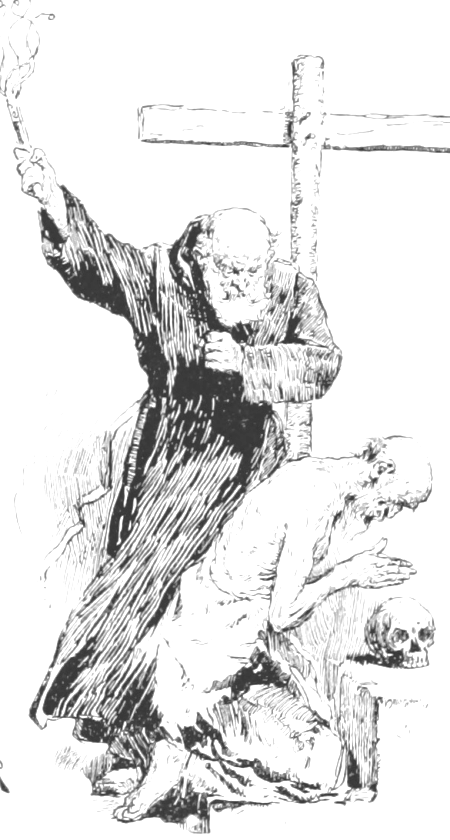
\includegraphics[scale=.5]{Flagellant}
\end{center}

\newpage

%%%%%%%%%%%%%%%%%%%%%%%%%%%%%%%%%%%%%%%%%%%%%%%%%%%%%%%%%%%%%%%%%%%%%%
%%%%  CIVILIZED %%%%%%%%%%%%%%%%%%%%%%%%%%%%%%%%%%%%%%%%%%%%%%%%%%%%%%
%%%%%%%%%%%%%%%%%%%%%%%%%%%%%%%%%%%%%%%%%%%%%%%%%%%%%%%%%%%%%%%%%%%%%%

\mysubsection{The Civilized Authority}{civilized-liturgies}

\flavor{
    Beauty  $\cdot$ Gems $\cdot$  Cities $\cdot$  Trade $\cdot$  Commerce $\cdot$  Filth $\cdot$  Pollution $\cdot$  Art $\cdot$  Music $\cdot$  Fermentation $\cdot$  Builders $\cdot$  Forge
}


\mybold{\myanchor{Liturgy of the Novitiates}{civilized-liturgy-novitiates}}

\mybullet{
    \item  Gain a +4 on all Skill:Math rolls.
    \item  When using a Bashing weapon, you may roll your \FOC instead of your \VIG or \DEX
    \item  Choose two Mysteries from this Authority or from your Small God (if applicable).  You may perform those Mysteries using your Faith.
}


  \begin{center}
  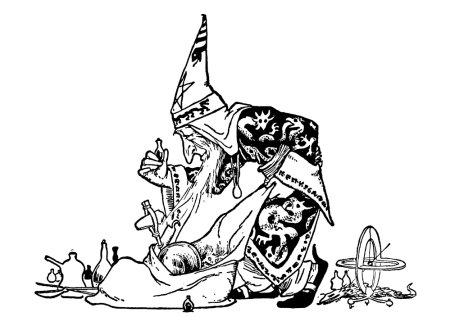
\includegraphics[scale=.5]{Civilized}
  \end{center}



\mybold{\myanchor{Liturgy of the Clerics}{civilized-liturgy-clerics}}

\mybullet {
    \item \mybold{Discerning Eye:} You know the exact worth of any gem or piece of art you can examine for uninterrupted Minutes.
    \item \mybold{Coins from Heaven:} You can convert Faith directly into coin.  You can only do this during a Vacation, and the money you generate does not count towards Glory.  Roll \DICE Faith.  For every 2 you get, gain 100fe (and lose the die); for every 3 you get, gain 25ag; for every 4 you get, gain 10au.    
    \item Choose two Mysteries from this Authority or from your Small God (if applicable).  You may perform those Mysteries using your Faith.
}

\cbreak


\mybold{\myanchor{Liturgy of the Apostles}{civilized-liturgy-apostles}}


\mybullet {
    \item You automatically succeed on all Skill:Math rolls
    \item \mybold{War Forge:} If you have access to a forge, you can create enough spears or shields (any combination) out of stones and earth.  You can create enough weaponry to arm a brigade of troops (1,500 - 4,000 soldiers)
    \item Choose two Mysteries from this Authority or from your Small God (if applicable).  You may perform those Mysteries using your Faith.
}

\begin{tcolorbox} [
  width=\linewidth,
  colbacktitle=silver,
  colback=white,
  coltitle=black,
  colframe=gainsboro,
  fonttitle=\fftext\normalsize,
  title=\mybold{The Civilized Mysteries},
  halign lower=center,
  sharp corners]
  \mylist {
     \item \mylink{Armor of the Gods}{arcana-mystery-armor-of-the-gods}
     \item \mylink{Clamp}{arcana-mystery-clamp}
     \item \mylink{Divvy}{arcana-mystery-divvy}
     \item \mylink{Exchequer}{arcana-mystery-exchequer}
     \item \mylink{Forgehammer}{arcana-mystery-forgehammer}
     \item \mylink{Hone}{arcana-mystery-hone}
     \item \mylink{Millworks}{arcana-mystery-millworks}
     \item \mylink{Package Neatly}{arcana-mystery-package-neatly}
   }
 \end{tcolorbox}



\mybold{\myanchor{Liturgy of the Saints}{civilized-liturgy-saints}}
\mybullet {
    \item \mybold{Urbane Temple:}  Once per Session during a Bivouac, you can create a gilded and runed pyramid 20m square at its base from thin air.  The pyramid may be built on land, water, or air - though it must be level with your feet when you build it.  The interior of the pyramid is Hallowed ground, and can safely house yourself and up to 12 other Allies. Spectral footmen flit around a banquet table groaning beneath ample food and drink  (no need for anyone to roll Provisions) - anyone who eats from this table heals full Grit and never get drunk.  Warm and comfortable beds lie behind privacy screens; anyone who chooses to rest regains full Flesh. Nothing can enter the pyramid without your permission, save for extraordinarily powerful beings (Arbiter's discretion).  The pyramid will last until the Bivouac ends; the stones and spectres disappear as if they had never been.
    \item Choose two Mysteries from this Authority or from your Small God (if applicable).  You may perform those Mysteries using your Faith.
}

\newpage

\mybold{\myanchor{Civilized Small Gods}{civilized-small-gods}}

\flavor{These seven Small Gods have the greatest number of worshipers on Acheron}


\GOD[Name=Balder,GodOf=Seraph of Beauty and Gems,Holy={a silver mirror}]

\GOD[Name=Gomorrah,GodOf=Archfiend of Cities,Holy={a single iron nail, often driven into the hand or wrist}]

\GOD[Name=Minerva,GodOf=Archon of Trade and Commerce,Holy={a knotted string, hung from the belt, useful for counting (like an abacus)}]

\GOD[Name=Nimlurun,GodOf=Fiend of Filth and Pollution,Holy={an iron vial of sewer water}]

\cbreak\bump

\GOD[Name=Ninkasi,GodOf={Seraph of Art, Music and Fermentation},Holy={an iron amulet hung from a necklace in the exact size and shape of a modern bottle opener}]

\GOD[Name=Ptah,GodOf=God of Builders,Holy={an amulet in the shape of an ankh}]

\GOD[Name=Vulcan,GodOf=Seraph of the Forge,Holy={a small crude homonculous, hammered from iron}]



\newpage

%%%%%%%%%%%%%%%%%%%%%%%%%%%%%%%%%%%%%%%%%%%%%%%%%%%%%%%%%%%%%%%%%%%%%%
%%%%  CTHONIC %%%%%%%%%%%%%%%%%%%%%%%%%%%%%%%%%%%%%%%%%%%%%%%%%%%%%%
%%%%%%%%%%%%%%%%%%%%%%%%%%%%%%%%%%%%%%%%%%%%%%%%%%%%%%%%%%%%%%%%%%%%%%

\mysubsection{The Cthonic Authority}{cthonic-liturgies}

\flavor{
    Murder $\cdot$  Betrayal $\cdot$  Shadows $\cdot$  Thieves $\cdot$  The Abyss $\cdot$  Death $\cdot$  Blood $\cdot$  Wyrms
}

\mybold{\myanchor{Liturgy of the Novitiates}{cthonic-liturgy-novitiates}}

\mybullet {
    \item Gain a +4 on all Skill:Salt rolls.
    \item When using a Fast weapon, you may roll your \FOC instead of your \DEX
    \item Choose two Mysteries from this Authority or from your Small God (if applicable).  You may perform those Mysteries using your Faith.
}



\mybold{\myanchor{Liturgy of the Clerics}{cthonic-liturgy-clerics}}

\mybullet {
    \item  \mybold{Sudden Strike:} If you gain Surprise on a Monster, you may attempt a Murder.  Use your \FOC to roll your Fight check.  See the Core Rules for the effects of Murder.
    \item  \mybold{Merfolk's Blessing:} You can breathe underwater with no ill effects.  If you invoke the mystery of \mylink{Mermaid's Breath}{arcana-mystery-mermaids-breath} on yourself, you can also swim as fast as you can run for the duration of the spell, even if you are carrying Significant Items.
    \item  Choose two Mysteries from this Authority or from your Small God (if applicable).  You may perform those Mysteries using your Faith.
}

\cbreak


\mybold{\myanchor{Liturgy of the Apostles}{cthonic-liturgy-apostles}}

\mybullet {
    \item  You automatically succeed on all Skill:Salt rolls
    \item  \mybold{Vampirism:} You can heal Flesh by drinking another sentient creature's blood.  You may perform this liturgy during a Breather or Bivouac.  The creature must be alive when you feast on them; the act of drinking their blood takes their life.  Heal yourself to full Flesh and Grit.
    \item  Choose two Mysteries from this Authority or from your Small God (if applicable).  You may perform those Mysteries using your Faith.
    
}

  \begin{center}
  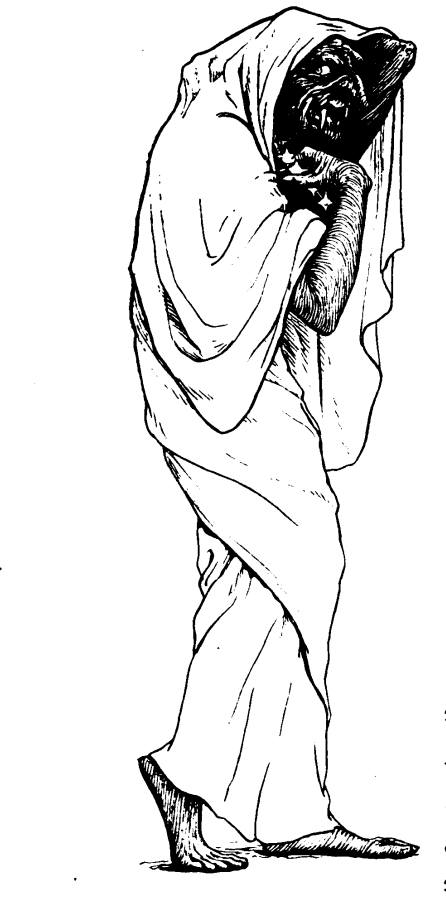
\includegraphics[scale=.5]{Cthonic}
  \end{center}

\begin{tcolorbox} [
  width=\linewidth,
  colbacktitle=silver,
  colback=white,
  coltitle=black,
  colframe=gainsboro,
  fonttitle=\fftext\normalsize,
  title=\mybold{The Cthonic Mysteries},
  halign lower=center,
  sharp corners]
  \mylist {
     \item \mylink{Abyssal Trident}{arcana-mystery-abyssal-trident}
     \item \mylink{Davy Jones's Locker}{arcana-mystery-davy-joness-locker}
     \item \mylink{Dredge}{arcana-mystery-dredge}
     \item \mylink{Excavate}{arcana-mystery-excavate}
     \item \mylink{Fade}{arcana-mystery-fade}
     \item \mylink{Mermaid's Breath}{arcana-mystery-mermaids-breath}
     \item \mylink{Sinister Stillness}{arcana-mystery-sinister-stillness}
     \item \mylink{Sound the Deeps}{arcana-mystery-sound-the-deeps}
   }
 \end{tcolorbox}



\mybold{\myanchor{Liturgy of the Saints}{cthonic-liturgy-saints}}

\mybullet {
    \item  \mybold{Shadowstep:} Once per Session, you can travel through shadow or darkness up to 10km away.  You need to have visited or must be able to see the destination, and there must be uninterrupted darkness or shadow between yourself and where you end up.  If the distance traveled is a Combat distance (Nearby, Far-Away, or Distant) the step takes a single Action, and you immediately gain Surprise.  If the distance is further away, you can travel the space in Minutes.
    \item  Choose two Mysteries from this Authority or from your Small God (if applicable).  You may perform those Mysteries using your Faith.
}

\cbreak

\mybold{\myanchor{Cthonic Small Gods}{cthonic-small-gods}}

\flavor{These seven Small Gods have the greatest number of worshipers on Acheron}


\GOD[Name=Arioch,GodOf=Fiend of Murder and Betrayal,Holy={a silver coin with a face on each side}]

\GOD[Name=Erebus,GodOf=Lord of Shadows,Holy={a piece of black gauze covering the mouth}]

\GOD[Name=Ik'tik'buboe,GodOf=The Drowned Sultan,Holy={a necklace made from crab's claws and nautical rope, tied in elaborate knots}]

\GOD[Name=Loki,GodOf=King of Thieves,Holy={an image of two snakes, circling one another to form an 'S' shape, and biting the tail of the other}]

\GOD[Name=Nyx,GodOf=Cousin of Death,Holy={a black lace shroud}]

\GOD[Name=Shezmu,GodOf=Prince of Blood,Holy={a vial of blood other than your own (preferably the blood of the one who indoctrinated you into the faith)}]

\GOD[Name=The King in Yellow,GodOf=Fiend of Illusion and Disguises,Holy={a yellow cowl and mask}]

\newpage

%%%%%%%%%%%%%%%%%%%%%%%%%%%%%%%%%%%%%%%%%%%%%%%%%%%%%%%%%%%%%%%%%%%%%%
%%%%  CUNNING %%%%%%%%%%%%%%%%%%%%%%%%%%%%%%%%%%%%%%%%%%%%%%%%%%%%%%
%%%%%%%%%%%%%%%%%%%%%%%%%%%%%%%%%%%%%%%%%%%%%%%%%%%%%%%%%%%%%%%%%%%%%%
\mysubsection{The Cunning Authority}{cunning-liturgies}

\flavor{
    Mysteries $\cdot$  Riddles $\cdot$  Wizards $\cdot$  Tricksters $\cdot$  Runes $\cdot$  Diplomacy $\cdot$  Inspiration $\cdot$  Knowledge
}



\mybold{\myanchor{Liturgy of the Novitiates}{cunning-liturgy-novitiates}}

\mybullet {
    \item Gain a +4 on all Skill:Lore rolls.
    \item When using a Throw weapon, you may roll your \FOC instead of your \DEX
    \item Choose two Mysteries from this Authority or from your Small God (if applicable).  You may perform those Mysteries using your Faith.
}


  \begin{center}
  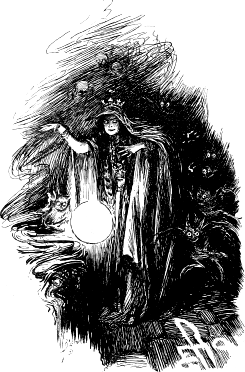
\includegraphics[scale=.5]{Cunning}
  \end{center}


\mybold{\myanchor{Liturgy of the Clerics}{cunning-liturgy-clerics}}

\mybullet {
    \item  \mybold{Sticky Fingers:} You can palm any hand sized item in your grasp.  As long as you're reasonably discrete, no need to roll.  Otherwise, \RB using your \FOC vs everyone's \INT
    \item  \mybold{Hecate's Blessing:} You may use your Faith to cast spells off of Fetishes
    \item  Choose two Mysteries from this Authority or from your Small God (if applicable).  You may perform those Mysteries using your Faith.
}



\mybold{\myanchor{Liturgy of the Apostles}{cunning-liturgy-apostles}}

\mybullet {
    \item  You automatically succeed on all Skill:Lore rolls
    \item  \mybold{That Kind of Face:} You are utterly forgettable.  Strangers will forget that they saw you or spoke to you; Scrying spells will fail when used upon you (including Sonorous Seeker); your written name becomes smudged and illegible on documents.  During Combat, if there is ever a choice to attack you or another, the Monster will always attack the other person.  This does not have any affect on the members of your Band, or people who have been in your company for longer than 3 Sessions. 
    \item  Choose two Mysteries from this Authority or from your Small God (if applicable).  You may perform those Mysteries using your Faith.
}


\begin{tcolorbox} [
  width=\linewidth,
  colbacktitle=silver,
  colback=white,
  coltitle=black,
  colframe=gainsboro,
  fonttitle=\fftext\normalsize,
  title=\mybold{The Cunning Mysteries},
  halign lower=center,
  sharp corners]
  \mylist {
     \item \mylink{Expertise}{arcana-mystery-expertise}
     \item \mylink{Illusion}{arcana-mystery-illusion}
     \item \mylink{Labyrinth}{arcana-mystery-labyrinth}
     \item \mylink{Memory Lane}{arcana-mystery-memory-lane}
     \item \mylink{Mirror Image}{arcana-mystery-mirror-image}
     \item \mylink{Paralysis}{arcana-mystery-paralysis}
     \item \mylink{Strange Copy}{arcana-mystery-strange-copy}
     \item \mylink{Twin}{arcana-mystery-twin}
   }
 \end{tcolorbox}

\mybold{\myanchor{Liturgy of the Saints}{cunning-liturgy-saints}}

\mybullet {
    \item \mybold{Doppelgänger:} If you have the opportunity to observe someone for Hours, you can flawlessly disguise yourself as that person - not even their family members will be able to tell the difference.  Your appearance to them is identical, though you don't have any access to their memories or abilities.  
    \item Choose two Mysteries from this Authority or from your Small God (if applicable).  You may perform those Mysteries using your Faith.
}

\newpage

\mybold{\myanchor{Cunning Small Gods}{cunning-small-gods}}



\flavor{These seven Small Gods have the greatest number of worshipers on Acheron}


\GOD[Name=Cthulhu,GodOf=Arbiter of Mysteries and Riddles,Holy={A piece of jewelry depicting an octopus}]

\GOD[Name=Hecate,GodOf=Archfiend of Wizardry,Holy={your Spellbook}]

\GOD[Name=Iktomi,GodOf=God of Tricksters,Holy={a small puppet, worn from the belt or neck}]

\GOD[Name=Mímir,GodOf=God of Runes,Holy={a necklace of runes scribed on tiles}]

\cbreak

\GOD[Name=The Grey Lords,GodOf=Archons of Diplomacy,Holy={a choker of dove feathers}]

\GOD[Name=The Muses,GodOf=Gods of Inspiration,Holy={a nine-pointed star, worn as an amulet or inscribed on a headband}]

\GOD[Name=Thoth,GodOf=God of Knowledge,Holy={a small book of scripture}]

\newpage

%%%%%%%%%%%%%%%%%%%%%%%%%%%%%%%%%%%%%%%%%%%%%%%%%%%%%%%%%%%%%%%%%%%%%%
%%%%  EMPYREAN %%%%%%%%%%%%%%%%%%%%%%%%%%%%%%%%%%%%%%%%%%%%%%%%%%%%%%
%%%%%%%%%%%%%%%%%%%%%%%%%%%%%%%%%%%%%%%%%%%%%%%%%%%%%%%%%%%%%%%%%%%%%%
\mysubsection{The Empyrean Authority}{empyrean-liturgies}

\flavor {
    Sunlight $\cdot$  Mountaintops $\cdot$  Heavens $\cdot$  Moonlight $\cdot$  Lightning $\cdot$  Tempests $\cdot$  Rains
}

\mybold{\myanchor{Liturgy of the Novitiates}{empyrean-liturgy-novitiates}}

\mybullet{
    \item Gain a +4 on all Skill:Eyeball rolls.
    \item When using a Shoot weapon, you may roll your \FOC instead of your \DEX
    \item Choose two Mysteries from this Authority or from your Small God (if applicable).  You may perform those Mysteries using your Faith.
}

\mybold{\myanchor{Liturgy of the Clerics}{empyrean-liturgy-clerics}}

\mybullet {
    \item \mybold{Kin to the Wind:} You may speak to the wind.  The wind will answer questions, but can only convey information to you about what it smelled and felt.  You can only use this ability while above ground.  In addition, you take -2 per die (minimum 1) damage from falling.
    \item \mybold{Lightning Affinity:} You take -2 damage per die (minimum 1) from electrical or lightning damage.  
    \item Choose two Mysteries from this Authority or from your Small God (if applicable).  You may perform those Mysteries using your Faith.
}

\mybold{\myanchor{Liturgy of the Apostles}{empyrean-liturgy-apostles}}

\mybullet {
    \item  You automatically succeed on all Skill:Eyeball rolls
    \item  \mybold{Eagle Eye:} When using a Shoot weapon, you automatically Crit whenever you successfully make a Fight check.
    \item  Choose two Mysteries from this Authority or from your Small God (if applicable).  You may perform those Mysteries using your Faith.
}

  \begin{center}
  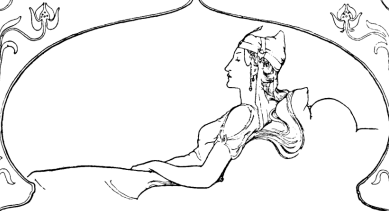
\includegraphics[scale=.5]{Empyrean}
  \end{center}

\begin{tcolorbox} [
  width=\linewidth,
  colbacktitle=silver,
  colback=white,
  coltitle=black,
  colframe=gainsboro,
  fonttitle=\fftext\normalsize,
  title=\mybold{The Empyrean Mysteries},
  halign lower=center,
  sharp corners]
  \mylist {
     \item \mylink{Children of Shul}{arcana-mystery-children-of-shul}
     \item \mylink{Glorious Sunburst}{arcana-mystery-glorious-sunburst}
     \item \mylink{Lightning}{arcana-mystery-lightning}
     \item \mylink{Lunacy}{arcana-mystery-lunacy}
     \item \mylink{Mountainhands}{arcana-mystery-mountainhands}
     \item \mylink{Rainburst}{arcana-mystery-rainburst}
     \item \mylink{Resonating Command}{arcana-mystery-resonating-command}
     \item \mylink{Thunderclap}{arcana-mystery-thunderclap}
   }
 \end{tcolorbox}

\mybold{\myanchor{Liturgy of the Saints}{empyrean-liturgy-saints}}


\mybullet {
    \item  \mybold{Healing Light:} If you are in sunlight, you will heal 1 Flesh at the bottom of each Moment (torchlight and moonlight don't count).  You cannot be slain unless you are in darkness or shadow.
    \item  Choose two Mysteries from this Authority or from your Small God (if applicable).  You may perform those Mysteries using your Faith.
}


\mybold{\myanchor{Empyrean Small Gods}{empyrean-small-gods}}

\flavor{These seven Small Gods have the greatest number of worshipers on Acheron}



\GOD[Name=Asura,GodOf=Seraph of Sunlight,Holy={polished mirrors or brass, hung from the neck or belt}]

\GOD[Name=Empress Wa,GodOf=God of the Heavens,Holy={a jade diadem}]

\GOD[Name=Raiden,GodOf=Lord of Lightning,Holy={two iron bracers with lightning bolts etched on them}]

\GOD[Name=Raimonds Mountainhand,GodOf=Seraph of the Mountaintops,Holy={3 iron spikes in the shape of icicles or teeth, hung from the neck}]

\GOD[Name=Shul,GodOf=Seraph of Moonlight,Holy={3 pearl earrings, hung from either ear}]

\GOD[Name=Tiamat,GodOf=Fiendish Prince of Tempests,Holy={a five pointed star, worn from a necklace}]

\cbreak

\GOD[Name=Tlaloc,GodOf=Archon of the Rains,Holy={a wreath of ferns and mosses}]

\newpage

%%%%%%%%%%%%%%%%%%%%%%%%%%%%%%%%%%%%%%%%%%%%%%%%%%%%%%%%%%%%%%%%%%%%%%
%%%%  ERRANT %%%%%%%%%%%%%%%%%%%%%%%%%%%%%%%%%%%%%%%%%%%%%%%%%%%%%%
%%%%%%%%%%%%%%%%%%%%%%%%%%%%%%%%%%%%%%%%%%%%%%%%%%%%%%%%%%%%%%%%%%%%%%
\mysubsection{The Errant Authority}{errant-liturgies}
\flavor{
    Games $\cdot$  Songs $\cdot$  Strength $\cdot$  Valor $\cdot$  Suffering $\cdot$  Freedom $\cdot$  Journeys $\cdot$  Homecomings $\cdot$  Treasures $\cdot$  Trials
}
\mybold{\myanchor{Liturgy of the Novitiates}{errant-liturgy-novitiates}}

\mybullet {
    \item Gain a +4 on all Skill:Travel rolls
    \item When using a Stabbing weapon, you may roll your \FOC instead of your \VIG or \DEX
    \item Choose two Mysteries from this Authority or from your Small God (if applicable).  You may perform those Mysteries using your Faith.
}


\mybold{\myanchor{Liturgy of the Clerics}{errant-liturgy-clerics}}

\mybullet {
    \item  \mybold{Breath of Freedom:} You can end a Markovian effect on yourself on a 1-3 (instead of a 1-2)
    \item  \mybold{Feats of Strength:} When you are rolling a \RB : \VIG check, use your \FOC instead
    \item  Choose two Mysteries from this Authority or from your Small God (if applicable).  You may perform those Mysteries using your Faith.

}



\mybold{\myanchor{Liturgy of the Apostles}{errant-liturgy-apostles}}

\mybullet {
    \item  You automatically succeed on all Skill:Travel rolls
    \item  \mybold{Unchained:} You cannot be bound by ropes, manacles, chains, etc. - they simply slip off your wrists, body, and feet at your command.  This won't help you if you're locked in a box or sealed in a coffin, nor will it help you with any "prisons of the mind"
    \item  Choose two Mysteries from this Authority or from your Small God (if applicable).  You may perform those Mysteries using your Faith.
}



\begin{tcolorbox} [
  width=\linewidth,
  colbacktitle=silver,
  colback=white,
  coltitle=black,
  colframe=gainsboro,
  fonttitle=\fftext\normalsize,
  title=\mybold{The Errant Mysteries},
  halign lower=center,
  sharp corners]
  \mylist {
     \item \mylink{Armor of Winds}{arcana-mystery-armor-of-winds}
     \item \mylink{Capture Wind}{arcana-mystery-capture-wind}
     \item \mylink{Corsair's Blade}{arcana-mystery-corsairs-blade}
     \item \mylink{Duelists' Wings}{arcana-mystery-duelists-wings}
     \item \mylink{Ropework}{arcana-mystery-ropework}
     \item \mylink{Shatter Bonds}{arcana-mystery-shatter-bonds}
     \item \mylink{Skald's Tongue}{arcana-mystery-skalds-tongue}
     \item \mylink{Vaulting Step}{arcana-mystery-vaulting-step}
   }
 \end{tcolorbox}


  \begin{center}
  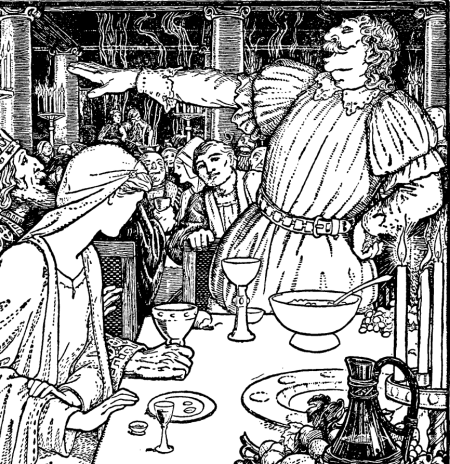
\includegraphics[scale=.5]{Errant}
  \end{center}


\mybold{\myanchor{Liturgy of the Saints}{errant-liturgy-saints}}

\mybullet {
    \item  \mybold{The Lash:} Once per Session, you can take any or all negative effects that would affect an Ally onto yourself instead.  This includes damage, Markovian effects, spell damage, etc.  You must declare you are suffering \mybold{The Lash} at the top of the Moment; any further effects can target you for the remainder of Combat.  You are allowed to roll your Guard, Saves, etc. independently of your Ally i.e. if your Ally failed to Guard against a Monster's attack, you can state the Monster is attacking you instead, and roll your Guard.
    \item  Choose two Mysteries from this Authority or from your Small God (if applicable).  You may perform those Mysteries using your Faith.
}


\mybold{\myanchor{Errant Small Gods}{errant-small-gods}}

\flavor{These seven Small Gods have the greatest number of worshipers on Acheron}


\GOD[Name=Balo,GodOf=Archon of Games and Contests,Holy={a leather bag of bone dice, hung from the neck or belt}]

\GOD[Name=Gilgamesh,GodOf=Lord of Strength and Valor,Holy={a pair of bull's horns, hung from the neck or worn as a helmet}]

\GOD[Name=Issek of the Jug,GodOf=Seraph of Suffering and Freedom,Holy={a broken pair of manacles}]

\GOD[Name=Kismet,GodOf=Arbiter of Journeys,Holy={a carved walking stick}]

\cbreak

\GOD[Name=Odysseus,GodOf=God of Homecomings,Holy={an iron wheel hanging from a bowstring necklace}]

\GOD[Name=Umwansh,GodOf=Lord of Many Treasures,Holy={a coin (gold is best) with a hole through the center, worn on a chain}]

\GOD[Name=Xbalanque and Hunahpu,GodOf=Twin Gods of Trials,Holy={two ears of dried corn (hung from a belt, around the neck, etc.)}]

\newpage

%%%%%%%%%%%%%%%%%%%%%%%%%%%%%%%%%%%%%%%%%%%%%%%%%%%%%%%%%%%%%%%%%%%%%%
%%%% HEATHEN %%%%%%%%%%%%%%%%%%%%%%%%%%%%%%%%%%%%%%%%%%%%%%%%%%%%%%
%%%%%%%%%%%%%%%%%%%%%%%%%%%%%%%%%%%%%%%%%%%%%%%%%%%%%%%%%%%%%%%%%%%%%%
\mysubsection{The Heathen Authority}{heathen-liturgies}

\flavor {
    Hearths $\cdot$  Gardens $\cdot$  Hunting $\cdot$  Glades $\cdot$  Fertility $\cdot$  Agriculture $\cdot$  Narcotics $\cdot$  "The Green Man" $\cdot$  Ancestors
}

\mybold{\myanchor{Liturgy of the Novitiates}{heathen-liturgy-novitiates}}

\mybullet {
    \item Gain a +4 modifier on Skill:Bushcraft rolls.
    \item For any narcotics you take, (a) the \UD only moves \DCDOWN if you roll a 1; (b) you add +4 to your Addiction roll, and (c) if you Overdose, treat the overdose as an d4 Iron (instead of Gold) Toxin
    \item Choose two Mysteries from this Authority or from your Small God (if applicable).  You may perform those Mysteries using your Faith.
}



\mybold{\myanchor{Liturgy of the Clerics}{heathen-liturgy-clerics}}

\mybullet {
    \item \mybold{Beastspeech:}  You can communicate with all mundane animals (though you can't command them).  They will answer your questions. Animals are guided by "base" desires for food and survival, so their answers are usually confined in that way i.e. "those 2 legged creatures on the road had no food" or "the green beast kills whatever it can get its hands on, we keep clear of it"
    \item \mybold{Sweetwater:} You can detoxify and restore food and drink with a touch.  The amount you can detoxify depends on how long you touch the object - an apple might become whole in Moments, but a well will take Hours to de-contaminate (Arbiter's discretion).  The touch can ameliorate Toxins one level down i.e.  it can turn a goblet containing a Gold toxin to a Silver, a Silver to an Iron, or remove an Iron Toxin completely.
    \item  Choose two Mysteries from this Authority or from your Small God (if applicable).  You may perform those Mysteries using your Faith.

}

  \begin{center}
  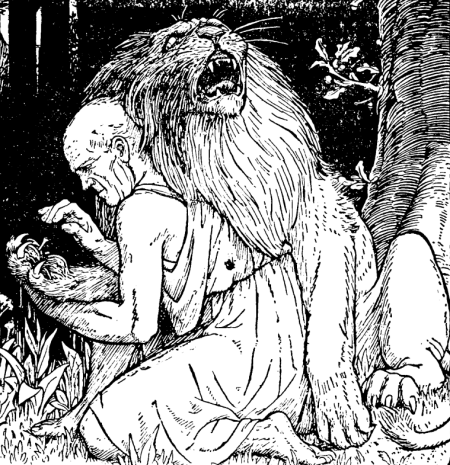
\includegraphics[scale=.5]{Heathen_1}
  \end{center}


\mybold{\myanchor{Liturgy of the Apostles}{heathen-liturgy-apostles}}

\mybullet {
    \item  You automatically succeed on all Skill:Bushcraft rolls
    \item  \mybold{Wisdom of the Ancients:} Once per Session, you can ask the Ancestors for aid.  If invoked during Combat, the Ancestors will fight on your behalf, granting you +4 on your Fight \RO.  Additionally, any physical damage you would take you can put on them instead.  They collectively have \LVL x2 Health and 0 Grit; when they have absorbed \LVL damage, they disappear. If invoked outside of Combat, the Ancestors will advise you on any question you might have.  They do not have any supernatural ability (they cannot Scry, for example), but you can benefit from their centuries of wisdom (Arbiter's discretion as to what that might mean).
    \item  Choose two Mysteries from this Authority or from your Small God (if applicable).  You may perform those Mysteries using your Faith.
}

\begin{tcolorbox} [
  width=\linewidth,
  colbacktitle=silver,
  colback=white,
  coltitle=black,
  colframe=gainsboro,
  fonttitle=\fftext\normalsize,
  title=\mybold{The Heathen Mysteries},
  halign lower=center,
  sharp corners]
  \mylist {
     \item \mylink{Barkskin}{arcana-mystery-barkskin}
     \item \mylink{Bloodvine}{arcana-mystery-bloodvine}
     \item \mylink{Butterfly Hurricane}{arcana-mystery-butterfly-hurricane}
     \item \mylink{Clearwater}{arcana-mystery-clearwater}
     \item \mylink{Elemental Spray}{arcana-mystery-elemental-spray}
     \item \mylink{Entangling Smoke }{arcana-mystery-entangling-smoke}
     \item \mylink{Hearthfire}{arcana-mystery-hearthfire}
     \item \mylink{Sporous Breath}{arcana-mystery-sporous-breath}
   }
 \end{tcolorbox}

\mybold{\myanchor{Liturgy of the Saints}{heathen-liturgy-saints}}

\mybullet {
    \item  \mybold{Elemental Kin:} You are immune to spells of the Elements paradigm.  Elementals and dragon breath deal -4 damage per die (minimum 1).
    \item  Choose two Mysteries from this Authority or from your Small God (if applicable).  You may perform those Mysteries using your Faith.

}

\cbreak


\mybold{\myanchor{Heathen Small Gods}{heathen-small-gods}}

\flavor{These seven Small Gods have the greatest number of worshipers on Acheron}


\GOD[Name=Brigid,GodOf=Seraph of Hearth and Gardens,Holy={a shillelagh}]

\GOD[Name=Cernunnos,GodOf=Archon of the Hunt,Holy={a tine of the antler of a game animal}]

\GOD[Name=Ildavir,GodOf=Lady of the Glade,Holy={a vial of clear water}]

\GOD[Name=Ishtar,GodOf=Lady of Fertility and Agriculture,Holy={an eight pointed star, usually worn as an amulet}]

\GOD[Name=Pilzesser,GodOf=Seraph of Hallucinogenic Plants and Fungi,Holy={a symbol of a pyramid with an eye at the top, and the letters "FNORD" along its base.  Worn as a necklace or headband}]

\GOD[Name=The Green Man,GodOf=Lord of the Wood,Holy={a crown of ivy or holly}]

\GOD[Name=Yan Oshoth,GodOf=Lady of Songs and Poetry (Ancestors),Holy={a small musical instrument}]




\newpage

%%%%%%%%%%%%%%%%%%%%%%%%%%%%%%%%%%%%%%%%%%%%%%%%%%%%%%%%%%%%%%%%%%%%%%
%%%%  Jötnar %%%%%%%%%%%%%%%%%%%%%%%%%%%%%%%%%%%%%%%%%%%%%%%%%%%%%%
%%%%%%%%%%%%%%%%%%%%%%%%%%%%%%%%%%%%%%%%%%%%%%%%%%%%%%%%%%%%%%%%%%%%%%
\mysubsection{The Jötnar Authority}{jötnar-liturgies}

\flavor {
Honorable Death $\cdot$  Battle Frenzy $\cdot$  Vengeance $\cdot$  Mercs And Assassins $\cdot$  Strategy And Combat $\cdot$  The Fire Of War $\cdot$  Ice And Snow
}

\mybold{\myanchor{Liturgy of the Novitiates}{jötnar-liturgy-novitiates}}

\mybullet {
    \item Gain a +4 modifier on \DEATH rolls
    \item When using a 2-Handed weapon, you may roll your \FOC instead of your \VIG or \DEX
    \item Choose two Mysteries from this Authority or from your Small God (if applicable).  You may perform those Mysteries using your Faith.

}

\mybold{\myanchor{Liturgy of the Clerics}{jötnar-liturgy-clerics}}

\mybullet {
    \item \mybold{Berserker:}  If you become Enraged, your beneficial effects are doubled i.e. you gain +8 to Fight and +8 to damage.  See the description of Enraged in the Core Rules.  At the end of Combat, you fall to 0 Flesh and must immediately make a \DEATH roll (before you receive any healing).
    \item \mybold{A Good Day to Die:} You can continue Fighting if you are Dying; however, each point of damage you take beyond 0 is a -1 modifier on your next \DEATH roll
    \item Choose two Mysteries from this Authority or from your Small God (if applicable).  You may perform those Mysteries using your Faith.
}

  \begin{center}
  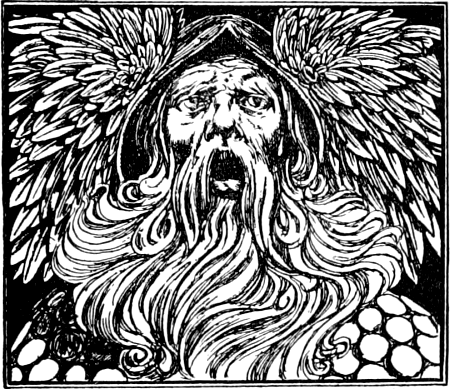
\includegraphics[scale=.5]{Jotnar}
  \end{center}


\mybold{\myanchor{Liturgy of the Apostles}{jötnar-liturgy-apostles}}

\mybullet {
    \item \mybold{Vengeance:}  If you are struck by a physical attack from a Monster, your next physical attack against that Monster automatically hits.
    \item \mybold{Bloody Boon:}  Once per Session, if you are reduced to 0 Flesh, you immediately regain \MAX Grit and can continue fighting. You must still roll your \DEATH tries at the top of the Moment as long as you are at 0 Flesh.
    \item Choose two Mysteries from this Authority or from your Small God (if applicable).  You may perform those Mysteries using your Faith.
}

\begin{tcolorbox} [
  width=\linewidth,
  colbacktitle=silver,
  colback=white,
  coltitle=black,
  colframe=gainsboro,
  fonttitle=\fftext\normalsize,
  title=\mybold{The Jötnar Mysteries},
  halign lower=center,
  sharp corners]
  \mylist {
     \item \mylink{Dirge}{arcana-mystery-dirge}
     \item \mylink{Extinguish}{arcana-mystery-extinguish}
     \item \mylink{Giantform}{arcana-mystery-giantform}
     \item \mylink{Incinerate}{arcana-mystery-incinerate}
     \item \mylink{Preserve}{arcana-mystery-preserve}
     \item \mylink{Ray of Fire}{arcana-mystery-ray-of-fire}
     \item \mylink{Trollblood}{arcana-mystery-trollblood}
     \item \mylink{Witness Me}{arcana-mystery-witness-me}
   }
 \end{tcolorbox}


\mybold{\myanchor{Liturgy of the Saints}{jötnar-liturgy-saints}}
\mybullet {
    \item  \mybold{Last Man Standing:}  During Combat, you can choose to enter "the final fugue" - while in this state, you are immune to all physical attacks, and make any Save tries.  At the end of Combat you immediately fall dead.
    \item  Choose two Mysteries from this Authority or from your Small God (if applicable).  You may perform those Mysteries using your Faith.
}

\newpage

\mybold{\myanchor{Jötnar Small Gods}{jotnar-small-gods}}

\flavor{These seven Small Gods have the greatest number of worshipers on Acheron}

\GOD[Name=Crom,GodOf=Arbiter of Honorable Death,Holy={The Devotee must name one of their weapons; this weapon will be used as their holy symbol}]

\GOD[Name=Cú Chulainn,GodOf=God of the Battle Frenzy,Holy={A headdress of raven or crow feathers}]

\GOD[Name=Justicia,GodOf=Seraph of Vengeance,Holy={An image or symbol of something the Devotee wants vengeance against}]

\GOD[Name=Kos,GodOf=Archon of Mercenaries and Assassins,Holy={3 rusted iron coins, sewn or welded to a bracelet on the dominant hand}]

\cbreak

\GOD[Name=Odin,GodOf=Archon of Strategy and Combat,Holy={3 interlocking triangles, worn as a necklace from a chain}]

\GOD[Name=Xotli,GodOf=Fiendish Prince of Fire,Holy={A red stone (agate, garnet, carnelian, red cinnabar, etc) worn on a choker.}]

\GOD[Name=Ymir,GodOf=Archon of Ice and Snow,Holy={Quartz stones affixed to a pair of leather or iron bracers}]

\newpage

%%%%%%%%%%%%%%%%%%%%%%%%%%%%%%%%%%%%%%%%%%%%%%%%%%%%%%%%%%%%%%%%%%%%%%
%%%%  MONSTROUS %%%%%%%%%%%%%%%%%%%%%%%%%%%%%%%%%%%%%%%%%%%%%%%%%%%%%%
%%%%%%%%%%%%%%%%%%%%%%%%%%%%%%%%%%%%%%%%%%%%%%%%%%%%%%%%%%%%%%%%%%%%%%
\mysubsection{The Monstrous Authority}{monstrous-liturgies}

\flavor{
    Cats $\cdot$  Toads $\cdot$  Reptiles $\cdot$  Arachnids $\cdot$  Monsters $\cdot$  Rats $\cdot$  Vermin $\cdot$  Birds
}


\mybold{\myanchor{Liturgy of the Novitiates}{monstrous-liturgy-novitiates}}

\mybullet {
    \item Gain a +4 modifier on Init rolls
    \item When using a Hard weapon, you may roll your \FOC instead of your \VIG
    \item Choose two Mysteries from this Authority or from your Small God (if applicable).  You may perform those Mysteries using your Faith.
}


\mybold{\myanchor{Liturgy of the Clerics}{monstrous-liturgy-clerics}}

\mybullet {
    \item You can fight with your fists (Unarmed Combat) using your \FOC instead of \VIG, with damage to match (see the section on Unarmed Combat in the core rules, but use your \FOC instead of \VIG for determining damage)
    \item \mybold{Tongue of Monsters:}  You can communicate with Aberrations, Giantkin, Goblinoids, and Graveborn.  They don't owe you any favors.
    \item  Choose two Mysteries from this Authority or from your Small God (if applicable).  You may perform those Mysteries using your Faith.
}



  \begin{center}
  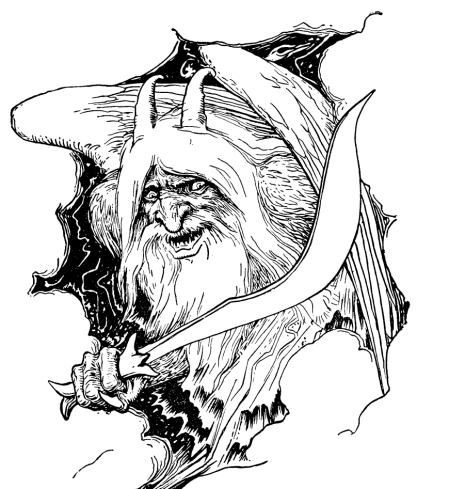
\includegraphics[scale=.5]{Monstrous_1}
  \end{center}



\mybold{\myanchor{Liturgy of the Apostles}{monstrous-liturgy-apostles}}

\mybullet {
    \item \mybold{Helping Hands:}  Two extra sets of arms sprout from your torso.  The arms cannot fight effectively, but they can hold things, and grant you a +4 on any rolls where extra arms might be useful (climbing, swimming, etc.)  You can sacrifice one of these arms to not take any damage from a physical attack, similar to Splintering a shield; doing so destroys the arm.  The arms feel no pain.  Wearing armor is difficult unless it is specially made, though you can fold your arms beneath your armor if you wish (obviously, you won't be able to utilize them at that point).
    \item \mybold{\myital{Acidum Sanguinem}} Your blood turns to acid.  If any physical attack hits Flesh, you spray an acid on everyone Close to you.  For d4 Moments, the acid deals d4 damage or removes 1 point of Soak.  If the person is wearing Armor, they don't take damage, but they must roll their Armor \UD at the bottom of every Moment for the duration of the effect.
    \item  Choose two Mysteries from this Authority or from your Small God (if applicable).  You may perform those Mysteries using your Faith.
}


\begin{tcolorbox} [
  width=\linewidth,
  colbacktitle=silver,
  colback=white,
  coltitle=black,
  colframe=gainsboro,
  fonttitle=\fftext\normalsize,
  title=\mybold{The Monstrous Mysteries},
  halign lower=center,
  sharp corners]
  \mylist {
     \item \mylink{Dragonbreath}{arcana-mystery-dragonbreath}
     \item \mylink{Harpy's Talons}{arcana-mystery-harpys-talons}
     \item \mylink{Serpent's Fang}{arcana-mystery-serpents-fang}
     \item \mylink{Slimeform}{arcana-mystery-slimeform}
     \item \mylink{Spidertongue}{arcana-mystery-spidertongue}
     \item \mylink{Tasty}{arcana-mystery-tasty}
     \item \mylink{Tattered Robe}{arcana-mystery-tattered-robe}
     \item \mylink{Undead Visage}{arcana-mystery-undead-visage}
   }
 \end{tcolorbox}


\mybold{\myanchor{Liturgy of the Saints}{monstrous-liturgy-saints}}

\mybullet {
    \item  \mybold{Telluric Immunity:}  In Combat, you can only be affected by magic weapons and spells
    \item  Choose two Mysteries from this Authority or from your Small God (if applicable).  You may perform those Mysteries using your Faith.
}


\mybold{\myanchor{Monstrous Small Gods}{monstrous-small-gods}}

\flavor{These seven Small Gods have the greatest number of worshipers on Acheron}


\GOD[Name=Bast,GodOf=Archon of Cats,Holy={a small bell without a clapper, worn on a choker}]

\GOD[Name=Bobugbubilz,GodOf=the Croaking Fane,Holy={3 desiccated frogs, worn from the belt or neck}]

\GOD[Name=Hhaaashh-Lusss,GodOf=Princess of Reptiles,Holy={snakeskin bracers}]

\GOD[Name=Mog,GodOf=Princess of Arachnids,Holy={a gossamer veil}]

\cbreak

\GOD[Name=Ptah-Ungurath,GodOf=Archfiend of Monsters,Holy={an amulet in the shape of an upside-down ankh}]

\GOD[Name=The Rat God,GodOf=Prince of Rats and Vermin,Holy={a mouse-skin glove worn on the dominant hand}]

\GOD[Name=Tyaa,GodOf=Archon of Birds,Holy={a short cloak of feathers}]

\newpage

%%%%%%%%%%%%%%%%%%%%%%%%%%%%%%%%%%%%%%%%%%%%%%%%%%%%%%%%%%%%%%%%%%%%%%
%%%%  RIGHTEOUS %%%%%%%%%%%%%%%%%%%%%%%%%%%%%%%%%%%%%%%%%%%%%%%%%%%%%%
%%%%%%%%%%%%%%%%%%%%%%%%%%%%%%%%%%%%%%%%%%%%%%%%%%%%%%%%%%%%%%%%%%%%%
\mysubsection{The Righteous Authority}{righteous-liturgies}
\flavor {
    Judgment $\cdot$  Punishment $\cdot$  Truth $\cdot$  Light $\cdot$  Time $\cdot$  Order $\cdot$  Law $\cdot$  Obedience $\cdot$  Protection $\cdot$  Oaths $\cdot$  Agreements
}


\mybold{\myanchor{Liturgy of the Novitiates}{righteous-liturgy-novitiates}}

\mybullet {
    \item Gain a +4 on all Skill:Listen rolls.
    \item When attacking with a Brawl weapon, you may roll \FOC instead of \VIG
    \item Choose two Mysteries from this Authority or from your Small God (if applicable).  You may perform those Mysteries using your Faith.
}



\mybold{\myanchor{Liturgy of the Clerics}{righteous-liturgy-clerics}}


\mybullet {
    \item \mybold{Holy Word:} You may \mylink{Curse the Unhallowed}{mystic-sacrament-curse-the-unhallowed} as the Sacrament of the same name.  You use your Faith instead of Grace to do this, and you do not need to know the Virtue of Seven Sacraments.
    \item \mybold{Binding Oath:}  Any contracts or agreements you enter into are bound by your Authority.  The contract is magically enforced; breaking the contract means the responsible party suffers permanent Anathema.  The Anathema can only be removed by the other party in the contract.
    \item  Choose two Mysteries from this Authority or from your Small God (if applicable).  You may perform those Mysteries using your Faith.
}

 \begin{center}
  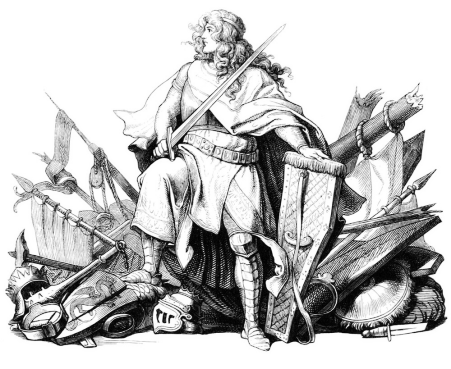
\includegraphics[scale=.5]{Righteous}
  \end{center}




\mybold{\myanchor{Liturgy of the Apostles}{righteous-liturgy-apostles}}

\mybullet {
    \item  You automatically succeed on all Skill:Listen rolls
    \item  \mybold{Spirit of Truth:} You are immune to lies and can see through any Illusion
    \item  Choose two Mysteries from this Authority or from your Small God (if applicable).  You may perform those Mysteries using your Faith.
}


\begin{tcolorbox} [
  width=\linewidth,
  colbacktitle=silver,
  colback=white,
  coltitle=black,
  colframe=gainsboro,
  fonttitle=\fftext\normalsize,
  title=\mybold{The Righteous Mysteries},
  halign lower=center,
  sharp corners]
  \mylist {
     \item \mylink{Crusader's Helm}{arcana-mystery-crusaders-helm}
     \item \mylink{Grounding Mantra}{arcana-mystery-grounding-mantra}
     \item \mylink{Holy Weapon}{arcana-mystery-holy-weapon}
     \item \mylink{Purging Fire}{arcana-mystery-purging-fire}
     \item \mylink{Revered Aegis}{arcana-mystery-revered-aegis}
     \item \mylink{Sacred Mail}{arcana-mystery-sacred-mail}
     \item \mylink{Satanic Verses}{arcana-mystery-satanic-verses}
     \item \mylink{Sonorous Seeker}{arcana-mystery-sonorous-seeker}
   }
 \end{tcolorbox}

\mybold{\myanchor{Liturgy of the Saints}{righteous-liturgy-saints}}

\mybullet {
    \item \mybold{Timestop:}  Once per Session, you can stop time for a Moment.  You can do this at any time - just before a killing blow falls, or just as a Philosopher is about to release a spell.  You may then immediately take action.  In Combat, you may take two Actions as normal as if this were a "normal" Moment.  Combat Actions automatically succeed (including Fight rolls), though the rule about a Fight action ending the Moment still applies.
    \item  Choose two Mysteries from this Authority or from your Small God (if applicable).  You may perform those Mysteries using your Faith.
}

\newpage

\mybold{\myanchor{Righteous Small Gods}{righteous-small-gods}}

\flavor{These seven Small Gods have the greatest number of worshipers on Acheron}


\GOD[Name=Anubis,GodOf=Fiend of Judgment and Punishment,Holy={a set of scales hung from a chain}]

\GOD[Name=Bahamut,GodOf=Lord of Truth and Light,Holy={an iron or silver circlet, embossed with an arrow pointing upwards}]

\GOD[Name=Chrontics,GodOf=Lord of Time,Holy={an amulet (silver preferred) embossed with a hammered hourglass}]

\GOD[Name=Marduk,GodOf=God of Law ,Holy={an unblinking eye worn on a linen headband}]

\cbreak

\GOD[Name=Mitra,GodOf=Seraph of Obedience and Protection,Holy={an iron thorn, coincidentally in the shape of a modern bullet, suspended from a chain around the neck}]

\GOD[Name=Týr,GodOf=Seraph of Order,Holy={an iron sleeve worn over the non-dominant hand (the hand is unable to hold anything)}]

\GOD[Name=Vár,GodOf=Seraph of Oaths and Agreements,Holy={a crystal vial containing the blood and spit of two Mortals who have struck a deal with one another}]


\newpage

%%%%%%%%%%%%%%%%%%%%%%%%%%%%%%%%%%%%%%%%%%%%%%%%%%%%%%%%%%%%%%%%%%%%%%
%%%%  RUINOUS %%%%%%%%%%%%%%%%%%%%%%%%%%%%%%%%%%%%%%%%%%%%%%%%%%%%%%
%%%%%%%%%%%%%%%%%%%%%%%%%%%%%%%%%%%%%%%%%%%%%%%%%%%%%%%%%%%%%%%%%%%%%
\mysubsection{The Ruinous Authority}{ruinous-liturgies}

\flavor{
Luck $\cdot$  Doom $\cdot$  Destruction $\cdot$  Hunger $\cdot$  Fate $\cdot$  Curses $\cdot$  Plagues
}

\mybold{\myanchor{Liturgy of the Novitiates}{ruinous-liturgy-novitiates}}

\mybullet {
    \item When attacking with a Brawl weapon, you deal +1 damage
    \item \mybold{Rending Strike:} Any weapon in your hands has the Rend attribute (see the Core Rules for details)
    \item Choose two Mysteries from this Authority or from your Small God (if applicable).  You may perform those Mysteries using your Faith.


}

\mybold{\myanchor{Liturgy of the Clerics}{ruinous-liturgy-clerics}}

\mybullet {
    \item When attacking with a Brawl weapon, you deal +3 damage instead of +1.
    \item \mybold{Shattering Strike:} In Combat, instead of attacking a person, you can attack their weapon instead.  If you successfully hit, the Monster must \RB : \VIG against your \FOC.  If they fail, the weapon is destroyed.  Magic weapons get a +4 to their rolls.
    \item Choose two Mysteries from this Authority or from your Small God (if applicable).  You may perform those Mysteries using your Faith.
}




\mybold{\myanchor{Liturgy of the Apostles}{ruinous-liturgy-apostles}}

\mybullet {
    \item When attacking with a Brawl weapon, you add +\LVL damage instead of +3.
    \item \mybold{Rotting Touch:} You can putrefy food and drink with a touch.  The amount you can putrefy depends on how long you touch the object - an apple might rot in Moments, but a well will take Hours to contaminate (Arbiter's discretion).  Anyone eating the food or water is afflicted with a Silver (d8) Toxin.
    \item Choose two Mysteries from this Authority or from your Small God (if applicable).  You may perform those Mysteries using your Faith.
}


 \begin{center}
  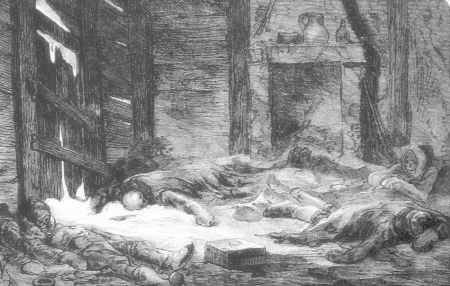
\includegraphics[scale=.5]{Ruinous}
  \end{center}


\begin{tcolorbox} [
  width=\linewidth,
  colbacktitle=silver,
  colback=white,
  coltitle=black,
  colframe=gainsboro,
  fonttitle=\fftext\normalsize,
  title=\mybold{The Ruinous Mysteries},
  halign lower=center,
  sharp corners]
  \mylist {
     \item \mylink{Doombolt}{arcana-mystery-doombolt}
     \item \mylink{Gaze of the Void}{arcana-mystery-gaze-of-the-void}
     \item \mylink{Kismet}{arcana-mystery-kismet}
     \item \mylink{Limbbreaker}{arcana-mystery-limbbreaker}
     \item \mylink{Shrikeblast}{arcana-mystery-shrikeblast}
     \item \mylink{Storm of Hammers}{arcana-mystery-storm-of-hammers}
     \item \mylink{Vermin Swarm}{arcana-mystery-vermin-swarm}
     \item \mylink{Wall of Gloom}{arcana-mystery-wall-of-gloom}
   }
 \end{tcolorbox}

\mybold{\myanchor{Liturgy of the Saints}{ruinous-liturgy-saints}}

\mybullet {
    \item \mybold{Killing Strike:} When attacking with a Brawl weapon, your damage die explodes. Add +\LVL damage to the final total.
    \item  Choose two Mysteries from this Authority or from your Small God (if applicable).  You may perform those Mysteries using your Faith.
}


\mybold{\myanchor{Ruinous Small Gods}{ruinous-small-gods}}

\flavor{These seven Small Gods have the greatest number of worshipers on Acheron}


\GOD[Name=Fortuna,GodOf=Seraph of Luck,Holy={A deck of cards}]

\GOD[Name=Nergal,GodOf=God of Dooms,Holy={an iron mask}]

\GOD[Name=Zuul,GodOf=Archfiend of Destruction,Holy={a ceramic circle broken in half, worn on the belt or a necklace}]

\GOD[Name=The Corpulent One,GodOf=God of Hunger,Holy={a necklace of teeth}]

\GOD[Name=The Morrigan,GodOf=Archon(s) of Fate,Holy={a triangle whose points extend into counterclockwise swirls, usually worn on a headband or scarf}]

\cbreak

\GOD[Name=Vecna,GodOf=Archfiend of Curses,Holy={a severed hand hung from the neck or belt}]

\GOD[Name=Xibalba,GodOf=Fiendish Prince of Fear,Holy={a white cowl and blank mask}]

  \newpage
  
\mysection{Mysteries}{arcana-mysteries}


\mysubsection{Civilized}{arcana-mystery-civilized}
\MYSTERY [
  Name = Armor of the Gods,
  Link = arcana-mystery-armor-of-the-gods,
  Paradigm = Force,
  Save = N,
  Duration = Session,
  Target = Self
]

You can't wear any other armor while wearing Armor of the Gods.  What the armor looks like is up to you, but it should be elaborate/brutal/gilded etc. - something that makes you stand out in a crowd.  Your \MD drops to d4; the \UD for the Armor depends on the number of \DICE invested: 1 d4; 2 d6; 3 d8; 4 d10; 5+ d12.  The Armor cannot be repaired; once its \UD is exhausted, the Armor disappears.


\MYSTERY [
  Name = Clamp,
  Link = arcana-mystery-clamp,
  Paradigm = Force,
  Save = Y (neg.),
  Duration = varies,
  Target = Nearby Target(s)
]

A clamp of red light appears over \DICE Monsters or objects you designate. The maximum width of the clamp is \DICE meters, and the clamp must be able to fit around the objects (so you wouldn't be able to clamp something to a floor or a wall).  The clamp will push the objects together until they are held securely, but it will not damage either object.  For example, you could clamp an orc to a chair or a sword to a table.  If one of the things clamped is a living thing, the creature can break free if they \RB : \VIG with a -\DICE penalty; otherwise, the duration depends on the number of dice spent:  1 [die]: Minutes; 2 \DICE: Days; 3 \DICE: Weeks; 4 \DICE: Months; 5 \DICE: Years; 6+ \DICE: Permanent.  Save negates.


\MYSTERY [
  Name = Divvy,
  Link = arcana-mystery-divvy,
  Paradigm = Entropy,
  Save = N,
  Duration = Permanent,
  Target = Close Target(s)
]

You can command something that's a mixture of different types (soup, coins, etc.) weighing no more than \DICE X50kg to separate into \DICE+1 categories.  The categories have to be clear and easily identifiable by inspecting them, and they have to be able to flow freely.  For example, you could split a soup into "vegetables" "broth" and "poison", or a pile of coins into "minted during the last century" and "older". You could not, however, split a pile of coins into "handled by Xerphion the Tyrant" and "not handled by Xerphion the Tyrant", as there's no way to tell just by inspecting them. You could not separate "a locked chest" and "its contents", because the items could not flow freely into separate piles.


\MYSTERY [
  Name = Exchequer,
  Link = arcana-mystery-exchequer,
  Paradigm = Entropy,
  Save = N,
  Duration = Instant,
  Target = Close Target(s)
]

You can convert up to \SUMDICE kg of coins into coins of another type of equivalent value (as a reminder, there are 100 coins in a kg, and 4kg of coins are 1 Significant Item). For example, if the \SUMDICE of your dice roll was 10 you could convert 1,000 iron pieces (10kg) into 100 silver pieces (1kg) or 10 gold pieces (1/10kg); or you could convert 10 gold pieces into 100 silver pieces or 1,000 iron pieces. Additionally, you can place up to \DICE X100kg of coins into "Hammerspace" for an indefinite period of time; the coins essentially cease to exist, have no Burden, and cannot be stolen or taken by others (though the existence of the coins can be divined through a Scry spell or similar).  You can retrieve the coins at any time (though you have to retrieve all of them at once).  The coins are also released upon your death, meaning that you might occasionally be a target of thieves.
You can combine the effects above (so you could convert money and store it in Hammerspace if you'd like).  You must cast this spell each time you want to put more coins into Hammerspace, but everything that's in Hammerspace is released upon your death.

  \begin{center}
  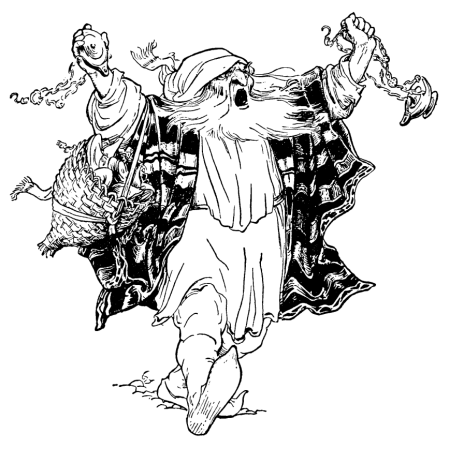
\includegraphics[scale=.5]{CivilizedArcana}
  \end{center}



\MYSTERY [
  Name = Forgehammer,
  Link = arcana-mystery-forgehammer,
  Paradigm = Force,
  Save = N,
  Duration = Session,
  Target = Self
]

A magical blacksmith's hammer appears in your hand that only you can wield.  The hammer deals \DICE+\DICE damage up to a maximum of 8. You fight with this weapon using your \FOC (instead of your \VIG).  You can repair the Max \UD of an Ally's armor during a Bivouac; for every \DCUP you repair in this way, the damage of the hammer goes down by 2. The Forgehammer can strike creatures who are only struck by magical weapons, but because there is no die to roll when dealing damage, it cannot Crit or be Fumbled.

Once the damage die is exhausted (reaches 0), the Forgehammer disappears.


\MYSTERY [
  Name = Hone,
  Link = arcana-mystery-hone,
  Paradigm = Force,
  Save = N,
  Duration = Combat or \SUM Minutes,
  Target = Close Target(s)
]

You run your hands over \DICE metal, stone, or wooden edges and hone them to a razor sharpness. If the object is a Bashing weapon, it deals +\DICE damage; if the object is a Stabbing or Chopping weapon, it deals +\DICE X2 damage. The edge must be smaller than your outstretched arms.

\MYSTERY [
  Name = Millworks,
  Link = arcana-mystery-millworks,
  Paradigm = Entropy,
  Save = N,
  Duration = Instant,
  Target = Close Target(s)
]

A tree no larger than \DICE X 5m tall and \DICE meters in diameter topples over, as if neatly cut. The result depends on the dice you invest. 1 \DICE: cut and broadly de-limbed, 2 \DICE: cut, de-limbed, debarked, 3 \DICE: cut, de-limbed, debarked, cut into planks as per your specifications, stacked, 4 \DICE cut, planed, de-limbed, debarked, cut into planks, stacked, sanded, and finished. Small limbs and offcuts will be piled for kindling. Alternatively, you can reduce the tree to sawdust or wood chips in 20-\SUMDICE minutes


\MYSTERY [
  Name = Package Neatly,
  Link = arcana-mystery-package-neatly,
  Paradigm = Entropy,
  Save = n/a,
  Duration = Concentration or Permanent,
  Target = Nearby Target(s)
]

Up to \DICE X250kg of nonliving objects, as you designate, are packed neatly. You must name the objects or their general category when you cast the spell ("those coins", "the contents of that room") If no packing materials are provided, the objects will be stacked into compact cubes, with the largest and most stable objects at the bottom. If chests, paper and twine, sacks, carts, etc. are provided, the spell will use them as you direct. The packages created will take up the minimum space possible, and will be remarkably sturdy. The spell will continue to pack objects for as long as you maintain concentration. The objects must be able to move freely. You could not use this spells to pack clothes someone was wearing. The objects will not lift more than 3m off the ground during the packing process.

\mysubsection{Cthonic}{arcana-mystery-cthonic}
\MYSTERY [
  Name = Abyssal Trident,
  Link = arcana-mystery-abyssal-trident,
  Paradigm = Force,
  Save = N,
  Duration = Session,
  Target = Self
]

A magical trident appears in your hand that only you can wield.  The trident is a 2-handed weapon that deals \DICE+\DICE damage up to a maximum of 12.   You fight with this weapon using your \FOC (instead of your \VIG).  Every time the trident deals damage, its damage goes down by 1. The trident can strike creatures who are only struck by magical weapons, but because there is no die to roll when dealing damage, it cannot Crit or be Fumbled. 

Once the damage die is exhausted (reaches 0), the Abyssal Trident disappears.

\MYSTERY [
  Name = Davy Jones's Locker,
  Link = arcana-mystery-davy-joness-locker,
  Paradigm = Prophesy,
  Save = N,
  Duration = Instant,
  Target = Close Target(s)
]

You must be near a body of water to use this liturgy (a river is OK, a puddle isn't).  You summon a chest up to \DICE meters in length, width, and height.  The box can hold up to \DICE X100kg in weight, or about 25 Significant Items (provided the box is big enough in terms of height, width, and depth i.e. you could lie a 2 meter long pole in a 2 [die] locker).  Once you seal the box and carve your name onto it, the waters will take the locker back beneath the surface, where it will disappear.  At any time, you can return to the same body of water and bring the locker back from the depths. Nothing else can bring the locker back from the deeps (not even the liturgy of Dredge) except your death.  When you die, the locker will wash up on shore within a few days for some lucky (or unlucky) soul to find.
If you place a living thing inside, it can breathe - but it will starve or die of thirst without food or water (incidentally, this is a great way to make \myital{vodyanoi})

\MYSTERY [
  Name = Dredge,
  Link = arcana-mystery-dredge,
  Paradigm = Mind,
  Save = N,
  Duration = Concentration,
  Target = Close or Nearby
]

The ground \DICE+\DICE meters in diameter (with you at the center) rumbles and quakes.  Buried or covered objects rise \DICE x5 meters to the surface.  Coins, stones, and roots will be pulled to the surface; if you cast it on water, sunken objects will rise to the surface and remain as long as you concentrate.  The objects cannot weigh more than \DICE x100kg.  

\MYSTERY [
  Name = Excavate,
  Link = arcana-mystery-excavate,
  Paradigm = Elements,
  Save = N,
  Duration = Instant,
  Target = Close
]

You can remove up to \DICE inorganic materials from a \DICE x5 meter cube just in front of your feet.  The materials could be "stone", "water", "dirt", etc. The materials disappear permanently. Objects that would be suspended in the material removed will obey the laws of physics - removing water will cause the surrounding water to rush in, removing dirt from around a chest will cause the chest to fall, etc.

\MYSTERY [
  Name = Fade,
  Link = arcana-mystery-fade,
  Paradigm = Mind,
  Save = Y (neg.),
  Duration = Markovian,
  Target = Nearby Target(s)
]

You can cause a Ally, Monster, or object to fade out of existence.  You can still see them, though they're insubstantial (like a ghost).  The target can't move, talk, or interact with the world in any way.  Not even magic can affect the target.  If the target is unwilling, it gets a Save to negate.  The duration is Markovian and depends on the number of \DICE invested.

  \begin{center}
  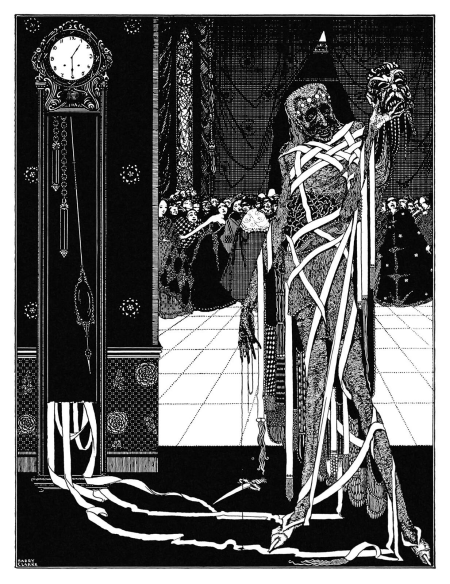
\includegraphics[scale=.5]{CthonicArcana}
  \end{center}


\MYSTERY [
  Name = Mermaid's Breath,
  Link = arcana-mystery-mermaids-breath,
  Paradigm = Biomancy,
  Save = Y (neg.),
  Duration = \SUM Minutes,
  Target = Self or Close Target(s)
]

For \SUMDICE Minutes, up to \DICE+1 Allies or Monsters (including yourself) can breathe water as if it were air.  They can only breathe water, however - breathing air will cause them to drown. Unwilling creatures get a Save to negate.  You must touch the Creature to bestow this mystery upon them. 

\MYSTERY [
  Name = Sinister Stillness,
  Link = arcana-mystery-sinister-stillness,
  Paradigm = Mind,
  Save = N,
  Duration = Combat or \SUM Minutes,
  Target = Close\, Nearby\, Far-Away\, or Distant
]

You can invoke this liturgy in an area  Close, Nearby, Far-Away, or Distant from yourself.  The air Close to the area takes on an unsettling air of silence.  Sound is not magically suppressed, but Monsters and creatures within its bounds feel that any sound they make will disturb something better left undisturbed.  Non-intelligent animals will not enter the area, and Monsters inside must make an immediate morale check. Thereafter, Saves against fear effects have a -\DICE and morale rolls suffer a -\DICE penalty (maximum -4).  A morale check is needed to enter or pass through the area of the spell.

\MYSTERY [
  Name = Sound the Deeps,
  Link = arcana-mystery-sound-the-deeps,
  Paradigm = Force,
  Save = N,
  Duration = Instant,
  Target = Close Target(s)
]

You slap your hand on the ground or the surface of the water.  The echoes of the tremor allow you to precisely know how deep and the approximate shape of bodies of water, chasms, shafts, clefts, mountain peaks, caverns, passages, etc.  up to a distance of \DICE x100m meters.  Additionally, you may use this to rouse \DICE+\DICE Allies Close, Nearby, Far Away, or Distant who are Sleeping, Knocked Out, etc. 

\newpage

\mysubsection{Cunning}{arcana-mystery-cunning}
\MYSTERY [
  Name = Expertise,
  Link = arcana-mystery-expertise,
  Paradigm = Mind,
  Save = N,
  Duration = \SUM Minutes,
  Target = Self
]

Name a Skill - it can be one of the 7 basic skills, or any other skill you choose (though you can't learn things that would not be contained in a well stocked library, or that are so rare that only a few people could teach them to you).  You are Skilled (d12+2) in that Skill for the spell's duration.  If you already know the Skill at a level of Skilled or better, add +\DICE x2 (up to a maximum of +4) to your Skill roll.

\MYSTERY [
  Name = Illusion,
  Link = arcana-mystery-illusion,
  Paradigm = Mind,
  Save = N,
  Duration = Varies,
  Target = See Below
]

You create an illusion of anything you desire. If anything touches the illusion, it will pass through it with no effect.  The illusion cannot be greater than \DICE x \DICE meters in size.  Think of the illusion as a perfectly accurate hologram that you are creating - the illusion can be heard in addition to being seen, can perform the same action over and over again, and can deliver messages, but it can't interact in a meaningful way or perform complex actions based on external forces. 

Each aspect of the illusion requires one or more Faith to cast:

\mybullet {
  \item You want the illusion to say up to \DICE + \DICE words or make \DICE + \DICE sounds (wailing, shouting, etc)
  \item You want the illusion to be a physical thing (hole in the ground, stone wall, orc guard, etc)
  \item You want the illusion to be able to move up to \DICE meters
  \item You want to cast the illusion on a living creature (disguise them as a beggar or a lamp post)
}

Note that there is some Arbiter's discretion here.  A guard pacing in front of a door might cost 2 \DICE (a physical thing moving back and forth 2
meters), but if you want the illusion of acrobats or pouncing lions it will be more costly.  A disguise cast on someone to appear to be a beggar might
cost 1 [die] (a living creature wearing the face and clothing of a random beggar), but disguising yourself as the king will be significantly harder.

The Illusion will last for \DICE Hours.  Anyone touching the illusion will immediately know it to be fake, but this doesn't cause the illusion to
disappear.  However, if the illusion is touched with an \mylink{Ego Weapon}{wizardry-ego-weapon}, it will immediately evaporate.

\MYSTERY [
  Name = Labyrinth,
  Link = arcana-mystery-labyrinth,
  Paradigm = Mind,
  Save = N,
  Duration = Combat or \SUM Minutes,
  Target = Self
]

You create a spiraling labyrinth of thought in your mind.  Anyone targeting you with Charm, Sleep, or any magical effect where the caster tries to read your mind or alter your memories must enter into a \RB : \FOC contest with you at a -\DICE penalty.  If they fail, they will be caught in your mind for the duration of the spell;  their physical body immediately catches the Vapors, and you can hear all their thoughts.

  \begin{center}
  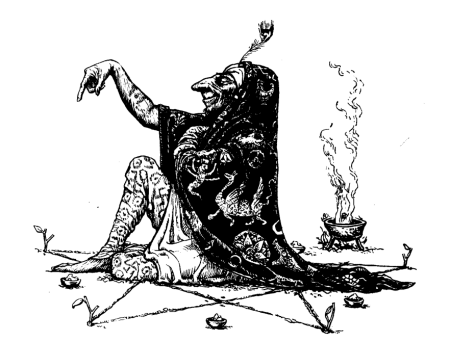
\includegraphics[scale=.5]{CunningArcana}
  \end{center}



\MYSTERY [
  Name = Memory Lane,
  Link = arcana-mystery-memory-lane,
  Paradigm = Mind,
  Save = Y (neg.),
  Duration = Varies,
  Target = Close Target(s)
]

You can create a memory (real or not) and embed it in the head(s) of up to \DICE creatures by touch.  Unwilling creatures may Save to negate the spell.  The memory must be short and distinct.  The memory will start to fade in a few days, but if you win a \RB : \FOC attempt against the victim (the victim has a -\DICE penalty) when you invoke the mystery, the memory will never fade, even if they lose all other memories (incidentally, this is is a really great way to create a ghost or poltergeist).

\MYSTERY [
  Name = Mirror Image,
  Link = arcana-mystery-mirror-image,
  Paradigm = Mind,
  Save = n/a,
  Duration = Minutes,
  Target = Self
]

You create \DICE illusory images of yourself, which move as you move and always stay Close to you. They are constantly stepping through each other, so that it is impossible to tell which is which. When an enemy attacks you, roll to see if they hit you or an image (equal chance). An image vanishes as soon as it suffers a solid impact (a blow from a mace, but also a slap). Area effects such as a dragon's breath will cause all images to instantly vanish (and you'll take fire breath damage, naturally).

\MYSTERY [
  Name = Paralysis,
  Link = arcana-mystery-paralysis,
  Paradigm = Mind,
  Save = Y (neg.),
  Duration = Markovian,
  Target = Close or Nearby Target(s)
]

Up to \DICE creatures of \DICE \HD or less must Save or be Paralyzed.  Sleeping creatures do not get a Save. The duration is Markovian and depends on the number of \DICE invested

\MYSTERY [
  Name = Strange Copy,
  Link = arcana-mystery-strange-copy,
  Paradigm = Mind,
  Save = N,
  Duration = \SUM Hours,
  Target = Close Target(s)
]

You reach into a mirror-like surface and pull out a copy of an object reflected in the mirror. The object that you pull out must be within reach of the mirror (as if it were a window), small enough to fit through the mirror (as if it were a window) and can't weigh more than \DICE x10kg. The mirror object looks and feels exactly like the object it copied, though it is a mirror image (so if you were to copy a book, the text would be backwards).  You can't copy any magical properties of the object, and you can only duplicate objects, not living things.  The object exists for \SUMDICE Hours.  If the object suffers a solid blow, it pops like a bubble.

\MYSTERY [
  Name = Twin,
  Link = arcana-mystery-twin,
  Paradigm = Mind,
  Save = N,
  Duration = \SUM Minutes,
  Target = Close Target(s)
]

You reach into a mirror-like surface and pull out a copy of yourself.  The mirrored surface has to be big enough for you to walk through - same height and same width, at least.  The copy behaves just like you, but it's illusory - anything that touches it will pass right through it, and it can't pick anything up or hold anything.  You can switch places with your mirror-self by stepping through the mirror - this dispels the illusion, and you appear wherever your mirror self is at the moment you step through.

\newpage

\mysubsection{Empyrean}{arcana-mystery-empyrean}
\MYSTERY [
  Name = Children of Shul,
  Link = arcana-mystery-children-of-shul,
  Paradigm = Prophesy,
  Save = Y (half),
  Duration = Session,
  Target = Self
]

You create \DICE small moons that circle the top of your head, casting moonlight Close and Nearby.  The shadows thrown by this moonlight give a +\DICE bonus (up to +4) to all Whispers made by Allies who are Close to you.  The moonlight will also activate abilities and powers that manifest in lunar rays (like lycanthropy), and throw light equivalent to \DICE x10 candles.

You can unerringly throw one these moons at Nearby Monsters every Moment, striking for 4 damage each (including creatures only struck by Magic weapons).  When you have no moons left, the spell ends.

The moons can be dispelled at any time, but can only be summoned once a Session.

\MYSTERY [
  Name = Glorious Sunburst,
  Link = arcana-mystery-glorious-sunburst,
  Paradigm = Elements,
  Save = Y (half),
  Duration = Combat or \SUM Minutes,
  Target = See Below
]

You raise your hands to the heavens and fire a flare up to 50m upwards, where it hovers providing bright sunlight to all areas Close, Nearby, and Far-Away.  You can command the sunburst to change color, move horizontally, or explode.  No shadows can be cast beneath the sunlight (meaning sneaking around is difficult if not impossible), and all invisible creatures and objects appear with a thin halo around them the color of the sun.  Anyone who performs the sacrament Curse the Unhallowed while under the Glorious Sunburst adds an additional +\DICE x2 to their damage; anyone Close to the sunburst if it explodes takes \SUMDICE+\DICE damage, Save for half.

\MYSTERY [
  Name = Lightning,
  Link = arcana-mystery-lightning,
  Paradigm = Elements,
  Save = Y (half),
  Duration = Instant,
  Target = Close or Nearby Target(s)
]

Forks of lightning erupt from your forehead, striking a Close or Nearby target for \SUMDICE+\DICE damage (Save for half). You can cause the lightning to "jump" up to \DICE-1 times to another creature or object Close by, provided they are conductive (iron armor, metal ladders, etc).  Magic swords aren't conductive.  You can "ping-pong" between two objects if you desire. Creatures struck by a secondary (or greater) lightning bolt take \DICE damage (no Save). Objects struck by the lightning bolt will become momentarily electrified, and deal a shock that could cause someone to lose their grip unless they \RO : \VIG + \FOC with a -\DICE penalty.

\MYSTERY [
  Name = Lunacy,
  Link = arcana-mystery-lunacy,
  Paradigm = Mind,
  Save = Y (neg.),
  Duration = Markovian,
  Target = Close or Nearby Target(s)
]

You invoke the madness of the moon.  \DICE creatures must immediately \RS : Sanity; if they do not have Sanity (Monsters, for instance) the creatures are permitted a Save.

The Lunacy is random for each Monster that fails its Save.  Roll a d4:  1) the Monster becomes Enraged at someone or something that isn't an Ally; 2) the Monster becomes Afraid of you and your Allies; 3) the Monster is Knocked Out; 4) the Monster suffers Anathema.  The duration is Markovian and depends on the number of \DICE used.

  \begin{center}
  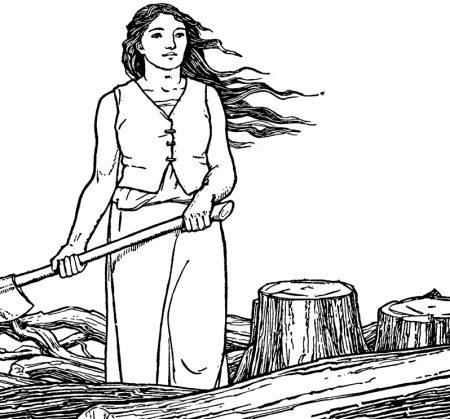
\includegraphics[scale=.5]{EmpyreanArcana}
  \end{center}


\MYSTERY [
  Name = Mountainhands,
  Link = arcana-mystery-mountainhands,
  Paradigm = Biomancy,
  Save = N,
  Duration = Session,
  Target = Self
]

Your hands enlarge and become stone.  Unarmed Attacks do +\DICE damage (up to a maximum of +4).  In addition, you can reach your hands into substances that might affect Flesh but not stone (fire, boiling water - OK.  Lava or acid - not OK).  Holding a stone in your hands allows you to speak to it as the Murk ability (see the Core Rules). 

Your hands must be empty (including rings and gloves) in order to invoke this mystery. You can only invoke this mystery once per Session.

\MYSTERY [
  Name = Rainburst,
  Link = arcana-mystery-rainburst,
  Paradigm = Elements,
  Save = n/a,
  Duration = Combat or \SUM Minutes,
  Target = See Below
]

You create a rainstorm in the surrounding area.  The rain extinguishes all fires (even magical ones) for the duration, prevents non-magical fires from starting, and heals Allies and Monsters alike for \SUMDICE Flesh (once at the moment of invocation).  The range is dependent on the number of \DICE invested: 1 Close; 2-3 Close and Nearby; 4-6 Close, Nearby, and Far-Away; 7+ Close, Nearby, Far-Away, and Distant.

\MYSTERY [
  Name = Resonating Command,
  Link = arcana-mystery-resonating-command,
  Paradigm = Mind,
  Save = Y (neg.),
  Duration = Markovian,
  Target = Nearby Target(s)
]

You shout a one word command at up to \DICE Close or Nearby target, who must obey (Save negates).  The target(s) must be able to understand your language.  The command resonates for a Markovian duration - if the Markovian die is not a 1 or a 2, they must Save again.  Each Moment after the first the target(s) gain an additional +1 to their Save.  The command cannot directly cause the target(s) harm or force them to commit a harmful action.  You could cause them to run into a trap they didn't know was there, or into a tactically disadvantageous position, but not off a cliff.

\MYSTERY [
  Name = Thunderclap,
  Link = arcana-mystery-thunderclap,
  Paradigm = Elements,
  Save = Y (neg.),
  Duration = Instant,
  Target = Far-Away or Distant
]

You can invoke this mystery somewhere Far-Away or Distant from yourself.  Monsters Close to the Thunderclap must immediately make a morale check with a -\DICE penalty, or become Afraid of you.  Additionally, Monsters become Deafened for \DICE Moments unless they make a Save with a -\DICE penalty.

\newpage

\mysubsection{Errant}{arcana-mystery-errant}
\MYSTERY [
  Name = Armor of Winds,
  Link = arcana-mystery-armor-of-winds,
  Paradigm = Entropy,
  Save = n/a,
  Duration = Session,
  Target = Self
]

Take \DICE Faith and put them "in reserve".  For the remainder of the Session, you may sacrifice one of these [die] to cause any single \mybold{physical} attack that would damage you to miss instead of hit.  You must sacrifice the [die] \myital{before} you roll your Guard or Save.  You can only use 1 [die] per Moment.  Any unused \DICE are lost at the end of the Session.  You can only invoke this mystery once per Session.

\MYSTERY [
  Name = Capture Wind,
  Link = arcana-mystery-capture-wind,
  Paradigm = Elements,
  Save = N,
  Duration = Concentration or Session,
  Target = See Below
]

A magical circle \DICE meters in radius extends from your fingertip in front of you. As long as you maintain concentration, you can absorb any wind passing through the circle. You can then collapse the spell. 

At any time during the Session, you can reactivate the circle to release the wind you absorbed.  The wind flows out at the same rate it entered. If you activate this spell in a light breeze for 5 minutes, the spell will release a light breeze over 5 minutes. The wind only flows from the circle, so anyone standing behind it is not affected (unless you release hurricane-force winds indoors). You can cancel the release at any time, which expends the spell as usual. If you go to 0 Flesh while the spell is still "reserved", it immediately activates facing a random direction.  

If the wind is a magical breath that would do damage (dragon's breath, etc.) your \SUMDICE must be equal to or greater than the sum of the damage, or the circle immediately collapses.  

\MYSTERY [
  Name = Corsair's Blade,
  Link = arcana-mystery-corsairs-blade,
  Paradigm = Force,
  Save = n/a,
  Duration = Session,
  Target = Self
]

A magical rapier appears in your hand that only you can wield.  The rapier deals \DICE+\DICE damage up to a maximum of 6.  You must make a successful Fight check using your \FOC (instead of \VIG or \DEX).  The Hero's Rapier ignores Armor and Soak, and while you wield it you always win Init. The rapier can strike creatures who are only struck by magical weapons, but because there is no die to roll when dealing damage, it cannot Crit or be Fumbled.  


  \begin{center}
  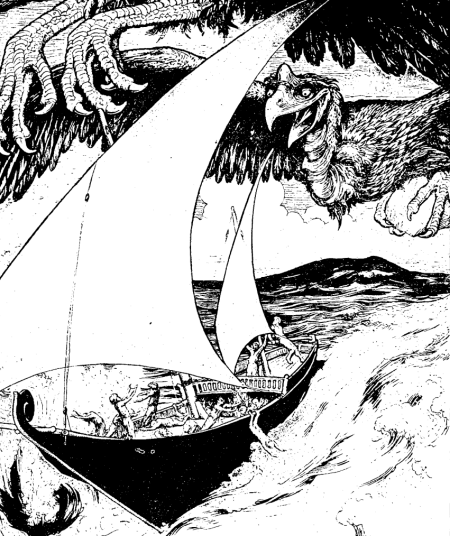
\includegraphics[scale=.5]{ErrantArcana}
  \end{center}



\MYSTERY [
  Name = Duelists' Wings,
  Link = arcana-mystery-duelists-wings,
  Paradigm = Biomancy,
  Save = n/a,
  Duration = Combat or \SUM Minutes,
  Target = Self or Close Target(s)
]

Tiny white wings sprout from the ankles and wrists of up to \DICE Allies.  They always win Init in Combat, and any falling damage is reduced by -\DICE per die.

\MYSTERY [
  Name = Ropework,
  Link = arcana-mystery-ropework,
  Paradigm = Entropy,
  Save = N,
  Duration = \SUM Minutes,
  Target = Close Target(s)
]

You summon a rope \DICE x50m in length.  You can command the rope to arrange itself into any shape and rise into the air in any orientation.  It can be climbed like a normal rope, and can support \DICE x100kg of weight.  Its ends do not need to be anchored to anything.

\MYSTERY [
  Name = Shatter Bonds,
  Link = arcana-mystery-shatter-bonds,
  Paradigm = Force,
  Save = n/a,
  Duration = Instant,
  Target = Close or Nearby
]

By invoking this mystery, you can sunder up to \DICE+\DICE bonds either Close or Nearby.  The bonds may be physical (shackles, chains, or locks) or mental (Charm, Command, Labyrinth, etc) at the Arbiter's discretion.

\MYSTERY [
  Name = Skald's Tongue,
  Link = arcana-mystery-skalds-tongue,
  Paradigm = Entropy,
  Save = n/a,
  Duration = Breather or Bivouac,
  Target = Close Target(s)
]

This mystery can only be invoked during a Breather or Bivouac.  You play a rousing song, recite part of an epic, or sing an ancient ballad.  You can heal up to \SUMDICE+\DICE Grit among all Allies who listen, divvied up any way you want.

\MYSTERY [
  Name = Vaulting Step,
  Link = arcana-mystery-vaulting-step,
  Paradigm = Force,
  Save = N,
  Duration = Instant,
  Target = Self
]

Your next \DICE+\DICE strides (about 1m each stride) land on a plane of Force the size of your foot.  The step can be taken in any direction up, down, sideways, or across (though you cannot pass through physical objects).  You can combine these in any way you want - stride 45 degrees into the air, take another step up, and a final step down (for example).  Your final step must be on a solid surface, or you fall. 


\mysubsection{Heathen}{arcana-mystery-heathen}
\MYSTERY [
  Name = Barkskin,
  Link = arcana-mystery-barkskin,
  Paradigm = Biomancy,
  Save = Y (neg.),
  Duration = Combat or \SUM Minutes,
  Target = Self or Close Target(s)
]

You or a creature you target is covered in heavy bark.  Weight is increased by \DICE x100kg and all physical damage is reduced by -\DICE for the duration of the spell, but you can't swim, jump, or run. If invoked on something already in deep water, mud, etc. the target will immediately sink at x\DICE the normal rate. Unwilling creatures get a Save to negate. 

\MYSTERY [
  Name = Bloodvine,
  Link = arcana-mystery-bloodvine,
  Paradigm = Biomancy,
  Save = N,
  Duration = Instant,
  Target = Close or Nearby Target(s)
]

This spell can only be used on a Monster who suffering from the Bleeding effect.  Vines erupt from the Monster's wounds, dealing \SUMDICE+\DICE damage (no Save).  If the damage kills the Monster, their corpse is entirely consumed in a bramble of vines

\MYSTERY [
  Name = Butterfly Hurricane,
  Link = arcana-mystery-butterfly-hurricane,
  Paradigm = Biomancy,
  Save = Y (neg.),
  Duration = Combat or \SUM Minutes,
  Target = Self
]

A whirling brightly colored mass of butterflies springs into being around you, cloaking you and anyone else Close to you.  Any ranged attacks fired into or out of the hurricane automatically miss (AoE effects like dragon's fire aren't affected).  Anyone inside of the hurricane must Save or become Befuddled for as long as they remain inside - you and up to \DICE Allies are immune.

\MYSTERY [
  Name = Clearwater,
  Link = arcana-mystery-clearwater,
  Paradigm = Elements,
  Save = n/a,
  Duration = Instant,
  Target = Self or Close Target(s)
]

This mystery can only be invoked during a Breather or a Bivouac.  You create \DICE draughts of cold, clear water that have one of the following effects:

\mynumlist {
    \item Restore \DICE Flesh
    \item Restore \SUMDICE Grit
    \item Immediately end the effect of a Toxin
    \item Immediately end the effect of a Disease
}

\MYSTERY [
  Name = Elemental Spray,
  Link = arcana-mystery-elemental-spray,
  Paradigm = Elements,
  Save = Y (half),
  Duration = Instant,
  Target = Close or Nearby Target(s)
]

You emit \DICE sprays of elements from your fingertips that you can split among \DICE Monsters.  For each Monster, if the \SUMDICE of the \DICE targeting the Monster is greater than the Monster's \HD, they take \DICE+\DICE fire damage.  If the \SUMDICE is twice the Monster's \HD or more, they also take \DICE+\DICE cold damage.  If the \SUMDICE is three times the Monster's \HD or more, they also take \DICE+\DICE lightning damage.  If the \SUMDICE is four times the Monster's \HD or more, they also take \DICE+\DICE acid damage.  Save for half.

\MYSTERY [
  Name = Entangling Smoke ,
  Link = arcana-mystery-entangling-smoke,
  Paradigm = Elements,
  Save = Y (neg.),
  Duration = Markovian,
  Target = Close or Nearby Target(s)
]

This spell requires the Narcotic: Pipeweed.  You breathe out a plume of smoke; up to \DICE creatures or objects are grabbed by tendrils of this smoke unless they Save.  Those who fail move at half speed (meaning it takes 2 Maneuvers to move somewhere Nearby; for Monsters, it means their speed is Slow if it isn't already).  Any Ally fighting this Monster gains a +\DICE bonus to Fight and Guard. The duration is Markovian and depends on the number of \DICE invested.

\MYSTERY [
  Name = Hearthfire,
  Link = arcana-mystery-hearthfire,
  Paradigm = Elements,
  Save = n/a,
  Duration = Bivouac,
  Target = Close Target(s)
]

During a Bivouac, you may perform up to \DICE effects, once per die (though you may choose an effect multiple times):
\mybullet {
\item Repair the \MAX \UD of an Allies armor to full
\item Provide Provisions for 1 Ally
\item Heal up to \DICE Flesh on 1 Ally
\item Prevent any Wandering Monsters from attacking your camp
}

  \begin{center}
  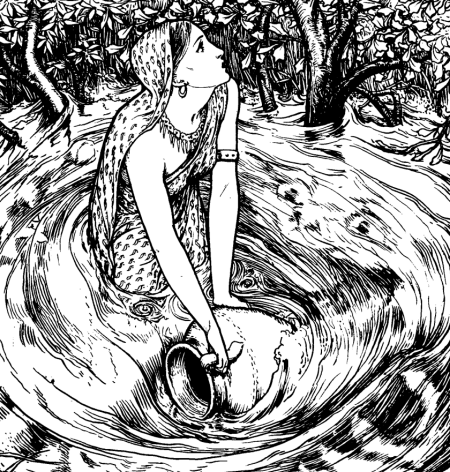
\includegraphics[scale=.5]{HeathenArcana}
  \end{center}



\MYSTERY [
  Name = Sporous Breath,
  Link = arcana-mystery-sporous-breath,
  Paradigm = Biomancy,
  Save = Y (neg.),
  Duration = Combat or \SUM Minutes,
  Target = Nearby Target(s)
]

You breathe a cloud of mushroom spores into an area Nearby.  All Allies and Monsters are affected by the Sporous Breath unless they make their Save.  The effects depend on the number of \DICE used: 1) all targets suffer Anathema; 2-3)  all targets are Woozy; 4-5 all targets are Befuddled; 6+) all targets are affected with an Iron (d4) Toxin.

Only yourself and Pooka are immune to the effects of the Sporous Breath.

\mysubsection{Jötnar}{arcana-mystery-jötnar}
\MYSTERY [
  Name = Dirge,
  Link = arcana-mystery-dirge,
  Paradigm = Death,
  Save = n/a,
  Duration = Concentration,
  Target = Close Target(s)
]

You begin droning a hero's dirge.  For as long as you concentrate, all Close and Nearby Allies gain a +\DICE bonus to their \DEATH checks, up to a maximum of +4.

\MYSTERY [
  Name = Extinguish,
  Link = arcana-mystery-extinguish,
  Paradigm = Elements,
  Save = N,
  Duration = Instant,
  Target = Close or Nearby Target(s)
]

Beams of slushy ice shoot from your outstretched hands and strike up to \DICE+\DICE targets.  Multiple beams can hit the same target.  If the target is on fire, the flame is immediately extinguished.  Flames the size of torches only require 1 [die]; people or animals would require 2 \DICE; bonfires and the like require 3+ \DICE at the Arbiter's discretion.

\MYSTERY [
  Name = Giantform,
  Link = arcana-mystery-giantform,
  Paradigm = Biomancy,
  Save = n/a,
  Duration = Combat or \SUM Minutes,
  Target = Self
]

You grow \DICE x 500cm in height, with strength to match.  Your Unarmed Attacks do an extra point of damage for every 2 \DICE you spend, and you can lift an additional \DICE x100kg.   If you are wearing Armor when you invoke Giantform, you take \MAX \UD in Flesh damage, and the Armor is ruined (drops to 0 \MAX \UD).  You are unable to use "normal" sized weapons while in Giantform.

\MYSTERY [
  Name = Incinerate,
  Link = arcana-mystery-incinerate,
  Paradigm = Elements,
  Save = N,
  Duration = See Below,
  Target = Close Target(s)
]

This mystery requires you to create a bonfire.  You can place up to \DICE inorganic objects into the fire weighing no more than \SUMDICE kg.  The objects are burned to a pile of enchanted ash, which can be harvested and stored as an Insignificant item.  When you wish the objects to become whole again, you must build a fire and sprinkle the ash inside of it; you can reach into the fire unharmed to pull the objects from the flames as they were when you placed them into the fire.  If you perish before the objects are retrieved, the ash reverts to normal, unenchanted ash and the objects are destroyed.


  \begin{center}
  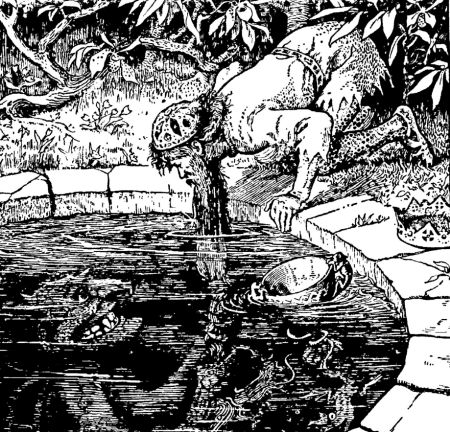
\includegraphics[scale=.5]{JotnarArcana}
  \end{center}



\MYSTERY [
  Name = Preserve,
  Link = arcana-mystery-preserve,
  Paradigm = Elements,
  Save = Y (neg.),
  Duration = varies,
  Target = Close Target(s)
]

By touching an object, you are able to freeze it for a period of time in order to preserve it.  If the object is an Ally or Monster, they must be lying completely still in order to use the liturgy.  Unwilling creatures get a Save.  While frozen, any toxins, diseases, bleeding, or negative effects are stopped for a period of time, depending on the number of dice spent.  You cannot end this liturgy willingly once it has begun, though it could be ended prematurely by great heat (a very large bonfire, for example) or by taking more than \SUMDICE points of damage, which will cause the object to shatter into many pieces.  

1 [die]: Minutes; 2-3 \DICE: Days; 4-5 \DICE: Weeks; 4 \DICE: Months; 6-7 \DICE: Years; 8+ \DICE: Permanent. 

\MYSTERY [
  Name = Ray of Fire,
  Link = arcana-mystery-ray-of-fire,
  Paradigm = Elements,
  Save = Y (neg.),
  Duration = Instant,
  Target = Nearby or Far-Away Target(s)
]

A narrow beam of fire shoots from your outstretched finger.  Make a Fight roll using your \FOC with a +\DICE modifier (up to +4); if you hit, the target catches fire for a Markovian duration if they fail a Save.  They are only allowed 1 Save.  They damage taken by the target is whatever is rolled on the Markovian die each Moment.  The beam of fire will also light flammable things alight.

\MYSTERY [
  Name = Trollblood,
  Link = arcana-mystery-trollblood,
  Paradigm = Death,
  Save = n/a,
  Duration = Combat,
  Target = Self
]

This mystery can be invoked at any time during Combat.  As long as you are alive, you regenerate +\DICE Flesh at the bottom of each Moment.  This regeneration is negated if the damage is from an acid or fire source. At the end of Combat, this mystery immediately ends (before you can take a Breather).

\MYSTERY [
  Name = Witness Me,
  Link = arcana-mystery-witness-me,
  Paradigm = Death,
  Save = n/a,
  Duration = Combat,
  Target = Self
]

This mystery can only be invoked in Combat.  For the remainder of Combat, you gain +\DICE x2 (up to +8) on your Fight checks, and deal +\SUMDICE damage when you hit (rolled each time along with your damage).  At the end of Combat, you immediately catch the Vapors and drop to 0 Flesh, and must make a \DEATH check.

\newpage

\mysubsection{Monstrous}{arcana-mystery-monstrous}
\MYSTERY [
  Name = Dragonbreath,
  Link = arcana-mystery-dragonbreath,
  Paradigm = Elements,
  Save = Y (half),
  Duration = Instant,
  Target = Nearby
]

You breathe out a gout of dragon's breath before you.  The breath deals \SUMDICE+\DICE damage to all creatures Nearby, Save for half damage (plus see below).  The type of breath is random, roll a d6 for the type of breath: 1) Fire (Red); 2) Acid (Black); 3) Frost (White); 4) Lightning (Blue); 5) Corrosive Gas (Green); 6) Void (Bone).  The additional effect of the dragon's breath is as follows:

\mybullet {
  \item \mybold{Red:}   Fire.  If you fail your Save, you catch fire.  Take d4 damage at the top of each Moment until you spend an entire Moment doing "stop, drop, and roll".  This can be shortened to a single Maneuver if someone helps you.
  \item \mybold{Black:}  Acid.  If you fail your Save, take d4 acid damage for d4 Moments
  \item \mybold{White:}  Frost.  If you fail your Save, you are knocked Prone
  \item \mybold{Blue:}  Lightning.  If you fail your Save \mybold{and} are wearing metal armor, take an additional 1 point of damage per die
  \item \mybold{Green:}  Corrosive gas.  If you fail your Save, reduce your Soak by 1, or roll your  Armor \UD
  \item \mybold{Bone:}  Void.  If you fail your Save, you catch the Vapors for d4 Markovian
}

\MYSTERY [
  Name = Harpy's Talons,
  Link = arcana-mystery-harpys-talons,
  Paradigm = Force,
  Save = n/a,
  Duration = Session,
  Target = Self
]

Your fingers sprout iron-hard talons.  The talons can strike for \DICE damage each up to a maximum of 4.  You can strike with both of these Talons in Combat at the same time; roll your Fight die twice using your \FOC (instead of your \VIG).  If both talons hit, the Monster is also afflicted with Bleeding.  Every time your talons deal damage, their damage goes down by 1 (you tell the Arbiter which Talon goes down in damage, either "left" or "right"); when \mybold{one} of the Harpy's Talons hits 0 damage, the talon disappears (you can still strike with the other talon, but it won't have the Bleeding effect). The talons can strike creatures who are only struck by magical weapons, but because there is no die to roll when dealing damage, it cannot Crit or be Fumbled

\MYSTERY [
  Name = Serpent's Fang,
  Link = arcana-mystery-serpents-fang,
  Paradigm = Biomancy,
  Save = n/a,
  Duration = Combat or \SUM Minutes,
  Target = Self
]

Make your Fight \RO using your \FOC.  If you succeed, you grapple a Monster and may immediately bite them with your fangs.  The Monster takes \DICE damage and begins Bleeding, unless they Save.  You may apply Toxins to your fangs, but if you do so you must \RS : \FOC or accidentally ingest the Toxin, with the appropriate negative effects.

\MYSTERY [
  Name = Slimeform,
  Link = arcana-mystery-slimeform,
  Paradigm = Biomancy,
  Save = n/a,
  Duration = \SUM Minutes,
  Target = Self
]

You transform yourself and all of your Gear into a slime.  You can absorb up to \SUMDICE+\DICE damage without any ill effects (damage after this goes straight to Flesh, and immediately ends the mystery).  You are unable to attack, talk, cast spells, etc while in Slimeform, but you can move at a the pace of a slow walk, climb walls, hang from the ceiling, and slip under the cracks of doors if you wish.

\MYSTERY [
  Name = Spidertongue,
  Link = arcana-mystery-spidertongue,
  Paradigm = Biomancy,
  Save = Y (neg.),
  Duration = Combat or \SUM Minutes,
  Target = Self
]

You can speak with spiders (and they can speak with you).  Small spiders know about water, wind, and bugs.  Larger spiders know about people (maybe they can tell them apart).  Big, dangerous spiders know all kinds of things.  Spiders will be friendly towards you, but if you attack them they'll fight back.  Additionally, your spittle becomes a Toxin whose power depends on the number of \DICE spent: 1-2 \DICE Iron Toxin; 3-4 \DICE Silver Toxin; 5+ \DICE Gold Toxin.  Your spittle is enough to poison a drink, a needle or syringe, or infect someone you might bite, but not enough to poison a knife or dagger.  The spittle becomes normal when the duration ends.


  \begin{center}
  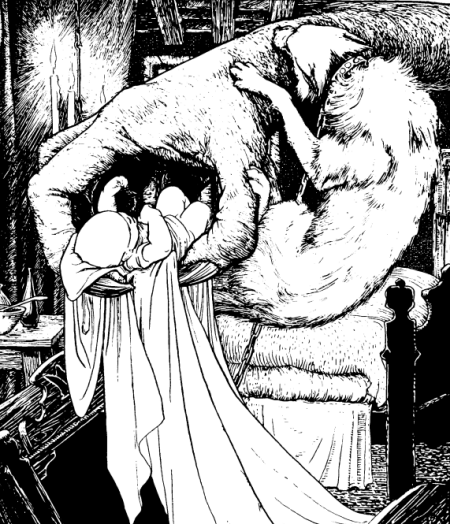
\includegraphics[scale=.5]{MonstrousArcana}
  \end{center}


\MYSTERY [
  Name = Tasty,
  Link = arcana-mystery-tasty,
  Paradigm = Biomancy,
  Save = N,
  Duration = Combat or \SUM Minutes,
  Target = Close Target(s)
]

The target object or Monster (alive or dead) smells delicious for the spell's duration.  The smell radiates Nearby in calm air, but can spread on the wind, or leave a trail.  Non-intelligent zoological creatures and swarms will be attracted to and attempt to eat the object or Monster first (even if they are supposed to be allies); intelligent creatures get a Save at a -\DICE penalty. 

\MYSTERY [
  Name = Tattered Robe,
  Link = arcana-mystery-tattered-robe,
  Paradigm = Entropy,
  Save = Y (neg.),
  Duration = Combat or \SUM Minutes,
  Target = Self
]

You must be wearing robes without armor to use this liturgy.  The edges of your robes form into \DICE tatters, each of which can be used as a weapon in combat in addition to your regular attack. The tatters deal no damage and each of their attacks must be rolled separately using your \FOC instead of your \VIG or \DEX - but if you hit the target begins Bleeding unless they make a Save.  You can split these attacks among as many Close opponents as you desire.

The tatters can also be used to hold small objects, as if they were each a prehensile tail.  Each tatter can hold up to 5kg of weight, but cannot attack if they are holding something.

\MYSTERY [
  Name = Undead Visage,
  Link = arcana-mystery-undead-visage,
  Paradigm = Death,
  Save = n/a,
  Duration = Combat or \SUM Minutes,
  Target = Self
]

You turn yourself into a hideous undead caricature of your "normal self".  You immediately become Unhallowed and gain the following effects, based on the number of \DICE spent:  1-2 you are immune to spells from the Mind Paradigm; 3-4 you are immune to Toxins; 5-6 you are immune to spells of the Force paradigm; 7+  you are immune to iron weapons.  These effects are cumulative.

You can only speak Graveborn for the duration of the spell.  Your Undead form prompts a Sanity or morale check among all who see you (Allies and Monsters alike), unless they have seen you in your Undead form before. 


\mysubsection{Righteous}{arcana-mystery-righteous}
\MYSTERY [
  Name = Crusader's Helm,
  Link = arcana-mystery-crusaders-helm,
  Paradigm = Force,
  Save = n/a,
  Duration = Session,
  Target = Self
]

You summon an ivory basinet, complete with crest, neck guard, and visor.  While worn, the Crusader's Helm protects you as a normal helmet (ignore certain Physical Wounds, etc), and you can absorb up to \DICE spells of the Mind paradigm without effect.  With the visor down you can detect Invisible creatures and are immune to Surprise (including the Drop).

\MYSTERY [
  Name = Grounding Mantra,
  Link = arcana-mystery-grounding-mantra,
  Paradigm = Elements,
  Save = Y (neg.),
  Duration = Markovian,
  Target = Close\, Nearby\, or Far-Away Target(s)
]

By invoking this liturgy, you shackle up to \DICE creatures to the ground.  They must be touching the ground already when you make the invocation.  The creatures must keep at least one limb touching the ground at all times.  If they attempt to run, they must \RB : \DEX with a -\DICE penalty.  If they are knocked Prone, they must \RB : \VIG with a -\DICE penalty to stand up.  Save negates.

\MYSTERY [
  Name = Holy Weapon,
  Link = arcana-mystery-holy-weapon,
  Paradigm = Force,
  Save = n/a,
  Duration = Session,
  Target = Self
]

A holy weapon (describe to the Arbiter) appears in your hands that only you can wield.  The weapon is a 2-handed weapon that deals \DICE+\DICE damage up to a maximum of 10.  In addition, you deal +\DICE damage against Unhallowed creatures. You fight with this weapon using your \FOC (instead of your \VIG). Every time the weapon deals damage, its damage goes down by 1; when it hits 0, the weapon disappears.  The Holy Weapon can strike creatures who are only struck by magical weapons, but because there is no die to roll when dealing damage, it cannot Crit or be Fumbled. 

\MYSTERY [
  Name = Purging Fire,
  Link = arcana-mystery-purging-fire,
  Paradigm = Elements,
  Save = N,
  Duration = \SUM Minutes,
  Target = See Below
]

This mystery requires you to create a bonfire.  Up to \DICE Allies can step into the flames of the Purging Flames; each Moment they remain inside of the fire; they take 2 damage to Flesh, but can activate 1 of the following effects:

\mynumlist {
    \item Immediately end a Markovian effect;
    \item Immediately remove a Curse;
    \item Immediately remove a non-serious Spiritual wound;
    \item Immediately purge a Toxin
}

Anyone inside of the Purging Flames cannot lie, and must answer truthfully any question asked of them


  \begin{center}
  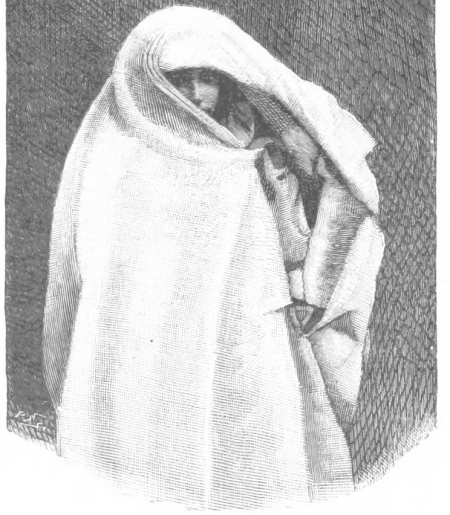
\includegraphics[scale=.5]{RighteousArcana}
  \end{center}



\MYSTERY [
  Name = Revered Aegis,
  Link = arcana-mystery-revered-aegis,
  Paradigm = Force,
  Save = n/a,
  Duration = Session,
  Target = Self
]

Take \DICE Faith and put them "in reserve".  You summon a brightly mirrored shield that can be Splintered (see the Combat Actions under Core Rules) up to \DICE times before it disappears.  Note that Splintering your shield is a Combat Action, and it ends your Moment; conversely, if you already took a Combat Action this Moment, you can’t Splinter the Revered Aegis.  Any unused \DICE are lost at the end of the Session.  You can only invoke this mystery once per Session.

\MYSTERY [
  Name = Sacred Mail,
  Link = arcana-mystery-sacred-mail,
  Paradigm = Force,
  Save = n/a,
  Duration = Session,
  Target = Self
]

You can't wear any other armor while wearing Sacred Mail.  The mail appears as a glimmering suit of chainmail.  Your \MD drops to d8; the \UD for the Armor depends on the number of \DICE invested:  1 d4; 2 d6; 3 d8; 4+ d10. The Mail cannot be repaired; once its \UD is exhausted, the Armor disappears.

\MYSTERY [
  Name = Satanic Verses,
  Link = arcana-mystery-satanic-verses,
  Paradigm = Entropy,
  Save = See Below,
  Duration = Instant,
  Target = Close
]

You shout a holy word, and books, scrolls, and parchment with writing on them burst into holy flame.  You can affect all writing in a \DICE meter radius centering on you.  If a Grimoire or Fetish is in possession of another (that is, on their person):
\mybullet {
    \item the Grimoire will not catch fire if the Philosopher can \RB : INT vs. your \FOC.  They gain a bonus modifier for every spell in the Grimoire, but a -\DICE penalty on their roll.
    \item the Fetish will not catch fire if the owner can \RB : \INT vs. your \FOC.  They may add the Fetish's \UD to their roll (and if they roll a 1 or a 2, the \UD moves \DCDOWN), but take a -\DICE penalty
}
If the Grimoire or Fetish is not in a persons' possession at the time the mystery is invoked, it does not get a Save.

Sigils will similarly catch aflame if the Arbiter is unable to \RB vs. your \FOC using a d10 (Minor), d16 (Major), or d24 (Primary) with a -\DICE penalty.

The mystery has no effect on Tattoos or spells written in the heads of Philosophers.  This mystery is indiscriminate in what writing it will set alight.


\MYSTERY [
  Name = Sonorous Seeker,
  Link = arcana-mystery-sonorous-seeker,
  Paradigm = Prophesy,
  Save = N,
  Duration = \SUM Minutes,
  Target = See Below
]

You create a fluttering star of light that twitters like a bird.  Name an object using up to \DICE+\DICE words - it can be a person ("the Stygian witch") or a thing ("the nearest body of water" or "the cask of Amontillado").  It has to be something you've seen clearly before.  Once named, the seeker will fly to it at the speed of an arrow and hover near it, chiming as loud as a bell.  If the object is not within the spell's range, it will try to find a similar object; otherwise, it disappears.


\mysubsection{Ruinous}{arcana-mystery-ruinous}
\MYSTERY [
  Name = Doombolt,
  Link = arcana-mystery-doombolt,
  Paradigm = Force,
  Save = Y (half),
  Duration = Instant,
  Target = Far-Away Target(s)
]

Target takes \SUMDICE+\DICE damage, Save for half. You do not need to see the target, but you do need to know their approximate location, and there must be a clear path a bolt could trace to reach them. The path can be as convoluted as required. The bolt can pass through gaps as small as a fist.  Note that this spell can only target Far-Away creatures.

  \begin{center}
  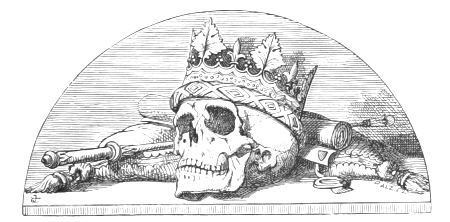
\includegraphics[scale=.5]{SkullLine}
  \end{center}



\MYSTERY [
  Name = Gaze of the Void,
  Link = arcana-mystery-gaze-of-the-void,
  Paradigm = Entropy,
  Save = Y (neg.),
  Duration = Instant,
  Target = Nearby or Far-Away Target(s)
]

A Monster disintegrates into nothingness. The number of \DICE invested must be twice the Monster's \HD + 1 (for example, to disintegrate a 1 \HD creature, you must invest 3 \DICE (1x2+1), a 2 \HD requires 5 \DICE, etc.) Monsters get a +2 to their Save; magical objects and magical monsters (dragons, unicorns, etc) get a +4 to their Save.



\MYSTERY [
  Name = Kismet,
  Link = arcana-mystery-kismet,
  Paradigm = Entropy,
  Save = n/a,
  Duration = Session,
  Target = See Below
]

Take \DICE Faith and put them "in reserve".  For the remainder of the Session, you may roll one of these [die] to modify \myital{any} \RO or \RB roll (by Ally or Monster alike) either plus or minus the \SUMDICE of the die roll.  You can only use 1 [die] per roll.  Regardless of the \SUMDICE of the [die], the Faith die is lost the moment it is rolled.  Any unused \DICE are lost at the end of the Session.  You can only invoke this mystery once per Session.

\MYSTERY [
  Name = Limbbreaker,
  Link = arcana-mystery-limbbreaker,
  Paradigm = Biomancy,
  Save = Y (neg.),
  Duration = Markovian,
  Target = Far-Away Target(s)
]

The target of this spell must have limbs.  With a snap of the fingers, \DICE of the target's limbs bend, crack, and break.  If an arm is broken, anything held in the hand is immediately dropped; if a leg is broken, the creature falls Prone; if both arms are broken, nothing can be picked up (and no spells can be cast); if both legs are broken, the Monster can only crawl.  The limbs remain broken for the Markovian duration, after which they immediately heal with no ill effects. Save negates.  Note that this spell can only target Far-Away creatures.

\MYSTERY [
  Name = Shrikeblast,
  Link = arcana-mystery-shrikeblast,
  Paradigm = Force,
  Save = Y (half),
  Duration = Instant,
  Target = Far-Away Target(s)
]

You let out a scream which shatters into shards of force.  The shards can lacerate up to \DICE  Far-Away Monsters and deal \SUMDICE+\DICE total damage (divided up any way you want).  If a Monster is killed by this spell, it will be suspended in the position it was killed for \SUMDICE Minutes by by the shards. A suspended creature is capable of bearing up to its own body weight in additional pressure before falling.  Note that this spell can only target Far-Away creatures.

\MYSTERY [
  Name = Storm of Hammers,
  Link = arcana-mystery-storm-of-hammers,
  Paradigm = Force,
  Save = Y (half),
  Duration = Concentration,
  Target = Far-Away Target(s)
]

Invisible hammers of Force strike up to \DICE Monsters from every direction.  Target Monsters take \DICE Bashing damage each, depending on how you split the die (Save for half).  The liturgy lasts for as long as you Concentrate.  Concentration and spell-casting is impossible while being struck by these hammers. Note that this spell can only target Far-Away creatures.

\MYSTERY [
  Name = Vermin Swarm,
  Link = arcana-mystery-vermin-swarm,
  Paradigm = Biomancy,
  Save = n/a,
  Duration = Concentration,
  Target = Close or Nearby
]

You summon a swarm of vermin that crawl up from the ground, walls, and ceiling.  The swarm can be directed for as long as you Concentrate and have a Base Speed (d16, 2 Maneuvers).  The swarm has \SUMDICE Health and deals \DICE damage to all Monsters Close to them provided a successful Fight roll is made (roll your \FOC for your Fight check).  Swarms take double damage from attacks that affect multiple targets, and share their Health equally as one "pool".  

\MYSTERY [
  Name = Wall of Gloom,
  Link = arcana-mystery-wall-of-gloom,
  Paradigm = Mind,
  Save = See Below,
  Duration = Markovian,
  Target = Nearby or Far-Away
]

You can anchor a barrier of pure darkness between three or more solid points up to \DICE meters in radius (for example: the 4 points of a door, two trees and the ground, across a hallway, etc).  Monsters that touch the blackness must immediately make a morale check with a -\DICE penalty or become Afraid for a Markovian duration.  If you spend 3 or more Faith, creatures that make their morale check that then continue through the wall must make a second Save; if they fail, they exit the wall the same way they came in (they will need to make a morale check again to touch the wall if they wish to try to move through it again).   


  \newpage
  
\mysection{Necromancy}{arcana-necromancy}

To reach through the veil between life and death is to plunge your hands into the black rivers surrounding the Isle of the Dead.  Necromancy is abhorrent to Hallowed creatures; there are those who insist that Necromancy defies \TheAuthority, while others insist that it would not be possible if it were not permitted.  


Necromancy requires the \mylink{Crux of Mojo}{mortal-crux-mojo}, and is divided into three loose groups:  Black Magic, Carnomancy, and Corpse Witching.  Each Necromantic spell has a "Target" associated with it - you must roll this number or greater using your Mojo.  You can try as many times as you like, but if you roll a 1 or a 2, your Mojo moves \DCDOWN.  Rolling your Mojo in this way is a Maneuver Action.


\mysubsection{Black Magic}{arcana-necromancy-black-magic}

\NECRO[
  Name=Born of the Grave,
  Link=necromancy-born-of-the-grave,
  Paradigm=Death,
  Save=N,
  Duration=Session,
  Target=4
]

Requires a snort of \mylink{Corpse Salt}{necromancy-corpse-salt}.  In addition to the Salt's narcotic abilities (see the Core Rules), you become as one born of the grave:

\mybullet {
    \item You take on a sickly/ghostly/rotting aspect.   You have \SUM additional Flesh while you are in this form.
    \item You are Unhallowed, breathe dirt as if it were air, have Darkvision, and can speak Graveborn fluently
    \item Any Allies that see you for the first time must roll their Sanity.  Monsters must roll their morale
    \item Shades and the Walking Dead will ignore you (unless you mess with them)
}

The effect can be ended at will; otherwise, it lasts until the end of the Session

\NECRO[
  Name=Crown of Thorns,
  Link=necromancy-crown-of-thorns,
  Paradigm=Death,
  Save=N,
  Duration=Session (see below),
  Target=5
]

A crown of blackberry thorns criss-crosses your forehead; blood leaks from your scalp.  Similar to the Virtue of Aura (see Core Rules), you use your Mojo as an Armor \UD in Combat.  Anyone who strikes you physically (including missile weapons) must Save or immediately take the Bleeding effect.  

The effect can be ended at will; otherwise, it lasts until the end of the Session or until your Mojo is exhausted.


  \begin{center}
  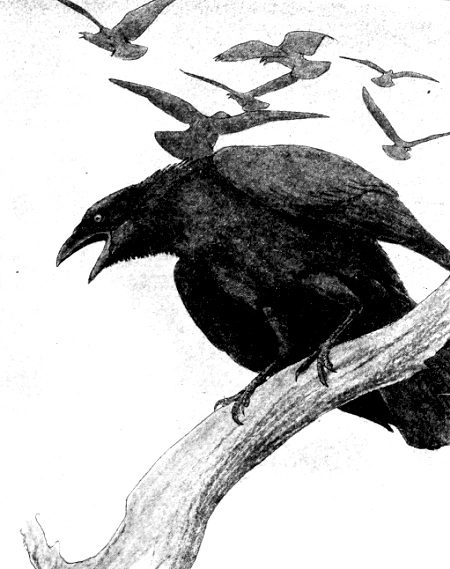
\includegraphics[scale=.5]{Crow}
  \end{center}


\NECRO[
  Name=Laughin' Jack,
  Link=necromancy-laughin-jack,
  Paradigm=Death,
  Save=N,
  Duration=0,
  Target=2
]

In a burst of blue flame and a whiff of brimstone, Laughin' Jack appears in your hand.  Jack appears as the blackened and burned skull of an infant, roughly the size of a grapefruit.  He emits a guttering, bluish corpselight from his eyes and mouth (treat as candlelight); if no one is looking at him, he whispers and chatters to himself in a language no one understands.  You may throw Jack (as a Throw weapon, obviously) using your \FOC instead of your \DEX.  Jack explodes for d4+1 damage on impact, and is able to strike creatures only hit by magic.  Throwing Jack is a Combat Action.



\NECRO[
  Name=Storm of Crows,
  Link=necromancy-storm-of-crows,
  Paradigm=Death,
  Save=Y (neg.),
  Duration=Concentration,
  Target=3
]

An inky murder of crows bursts from the ground in a whirling cloud, cloaking you and anyone Close to you.  For as long as you maintain Concentration, any ranged attacks fired into or out of the hurricane automatically miss (AoE effects like dragon's fire aren't affected).  

\mysubsection{Carnomancy}{arcana-necromancy-carnomancy}

\example{
    Using Carnomancy on an Ally requires them to make a \RS Sanity check. 
}


\NECRO[
  Name=Canopic Jar,
  Link=necromancy-canopic-jar,
  Paradigm=Death,
  Save=N,
  Duration=Session,
  Target=4
]

You pull out yours or an Ally's stomach, intestines, lungs, or liver and store them in Hammerspace.  You can only store 1 organ per person at a time.  For each person after the first, the Target increases by +1 (for example, you could store your stomach in Hammerspace, the paladin's lungs [the Target would 5], and the wizard's stomach [the Target would be 6]).  While the organ is stored in Hammerspace, you (or your Ally) are Unhallowed.  Unwilling participants get a Save.

\mybullet {
    \item \mybold{Stomach:}   You do not need to eat or drink
    \item \mybold{Intestines:}  You can heal Grit even if an effect (like a specific wound) would normally prevent you from doing so
    \item \mybold{Lungs:}  You no longer need to breathe (this makes talking impossible)
    \item \mybold{Liver:}  You are not affected by any ingested Toxins.  If performed while under the effect of the Toxin, the Toxin is removed from the body along with the liver and placed in Hammerspace.  The Toxin must be dealt with when the liver is (presumably) returned to the body.
}


\NECRO[
  Name=Corpse Tongue,
  Link=necromancy-corpse-tongue,
  Paradigm=Death,
  Save=N,
  Duration=Session or \SUMDICE Minutes,
  Target=3
]

Using Corpse Tongue requires \mylink{Corpse Salt}{necromancy-corpse-salt}

\mybullet{ 
    \item \mybold{Corpse Smoke:} The Corpse Salt is mixed with pipeweed and Smoked (eliminating its Narcotic effects).  You gain the languages, memories, and Skills of the corpse for the rest of the Session (but not any spells, supernatural abilities, Virtues, etc.).  If the creature's particularly powerful (Arbiter's discretion), you must Save vs. Hexes or gain some aspect of the creature's personality for the duration of the Session.  If the creature was over 100 years old, you must \RS : Sanity.  
    \item \mybold{Speak with Dead:}  You spread the Corpse Salt on a flat surface (be careful it doesn't blow away!)  The corpse will answer questions for \SUMDICE Minutes (the Arbiter will start a timer).  The dead only speak in Graveborn.  They will answer honestly, but the words tend to be cryptic and unhelpful, especially if the creature has no reason to help you.  Corpses usually don't remember exactly how they died.
}


\NECRO[
  Name=Covenant of Blood,
  Link=necromancy-blood-sacrament,
  Paradigm=Death,
  Save=Y (see below),
  Duration=see below,
  Target=2 (see below)
]

The Covenant of Blood allows you to do the following:

\mybullet {
    \item You can anoint someone with blood from your pricked finger.  They are Unhallowed until the end of the Session.  Unwilling creatures get a Save.
    \item Add +4 to the Target (6).  This rite can only be performed during a Bivouac.  You transfer blood from one creature to another; both creatures must be alive at the time of the transference.  Each Moment, the "donor" loses 1 point of Flesh, and the "recipient" gains 1 point of Flesh.  If the donor is brought to 0 Flesh during the transference, the recipient must Save vs Doom or fall to 0 Flesh, prompting a roll of their \DEATH
    \item Add +8 to the Target (10),  You heal from drinking another sentient creature's blood.  You may perform this liturgy during a Breather or Bivouac.  The creature must be alive when you feast on them; the act of drinking their blood takes their life.  Heal yourself to full Flesh and Grit.

}


  \begin{center}
  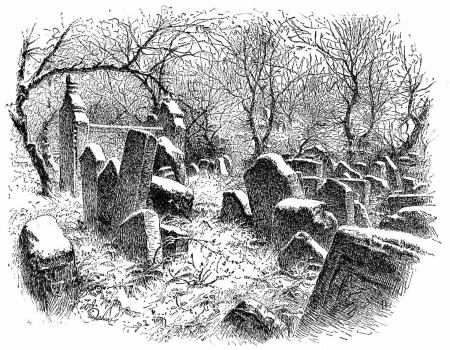
\includegraphics[scale=.5]{Graveyard}
  \end{center}


\NECRO[
  Name=Knit Flesh,
  Link=necromancy-knit-flesh,
  Paradigm=Death,
  Save=N,
  Duration=0 or Session,
  Target=2 (see below)
]

\mybullet {
    \item You heal 1 \HD of Flesh on a single creature. The healed flesh will appear gray and bloodless; wounds are sealed with wire and crude staples.  Horrible scars are usually left behind. You can only do this once per creature during a Breather or Bivouac (before you restore any Mojo).
    \item Add +1 to the Target (3).  You can remove someone's face and wear it as a mask.  You will look exactly like them (but not have their memories, skills, abilities, etc.).  The person does not need to be alive to perform this necromancy, but they do need to keep fucking still for a few minutes.
    \item Add +2 to the Target (4).  You stitch a lost limb or hand to a stump.  This requires an available limb of the appropriate size.  The limb rots quickly and a new one needs to be attached each Session.  The Mystic also can "feel" what the limb feels (i.e. they can tell if the creature is holding something [but not what], if the creature is walking or running, etc).  While the stitched limb is attached, the creature is Unhallowed.
}


\mysubsection{Corpse Witching}{arcana-necromancy-corpse-witching}

\example{
    Corpse Witching must be performed on a corpse, no more than 7 days dead (by the law of \TheAuthority).  Corpse Witching consumes (destroys) the corpse
}


\NECRO[
  Name=Corpse Salt,
  Link=necromancy-corpse-salt,
  Paradigm=Death,
  Save=N,
  Duration=0,
  Target=2
]

You create d4 \UD of Corpse Salt, a coarse and gritty distillation that can be stored in a tiny pouch or vial.  Corpse Salt is a necessary component in certain Necromantic arts, and a Narcotic sought out by Philosophers (see Narcotics under the Core Rules).


\NECRO[
  Name=Death Scythe,
  Link=necromancy-death-scythe
  Paradigm=Death,
  Save=N,
  Duration=Session or Until Exhausted,
  Target=4
]


The corpse disintegrates as you pluck a black scythe from its center of mass. The scythe is 2 Handed and does d8 damage; this d8 is a \UD - when you exhaust the \UD, the scythe disappears.  Against Monsters of the same type, the scythe has the Weapon Trait: Cleave (for example, a scythe made from a troll corpse would have Cleave against trolls.) The scythe is only usable by you and counts as a magic weapon; it does not count as a Significant Item. You must make a successful Fight check using your \FOC (instead of \VIG or \DEX) to hit with the weapon.

\NECRO[
  Name=Exploding Corpse,
  Link=necromancy-exploding-corpse,
  Paradigm=Death,
  Save=N,
  Duration=Combat,
  Target=3
]

A corpse Close or Nearby to you explodes in a shower of bone and blood.  Anyone Close to the corpse must Save vs Hexes or take \SUMDICE damage.  Makes a really big fucking mess.



\NECRO[
  Name=Zombie,
  Link=necromancy-zombie,
  Paradigm=Death,
  Save=N,
  Duration=Session or Conc.,
  Target=5
]

\mybullet{
    \item \mybold{Slave:} You raise a corpse to help with mundane tasks, test for traps, etc.  The corpse moves very slowly (d3 \MD) but doesn't need to eat, sleep, rest, or breathe.  The corpse cannot Fight or Guard, and any damage to it (including Curse the Unhallowed) immediately destroys the Zombie.  The Zombie has the strength of a normal person and can carry 25kg worth of stuff without tiring, but it'll need to be strapped to them (in a backpack or whatever).  Arbiter gets final say on what's allowed. The corpse can obey one word commands i.e. "dig", "sit", "go", "stop", etc.  The corpse can only understand Graveborn. It is completely mindless and extremely literal. The corpse will obey your last command until the spell's duration expires.  When the spell ends, the corpse falls to the ground and is immediately consumed.

    \item \mybold{Warrior:}  Creating a Warrior adds +3 to the Target (8).  The corpse is raised and will fight for you for as long as you maintain Concentration.  The Zombie uses your Mojo to Fight and Guard; you can raise as many Warriors as you wish, but they each use your Mojo to Fight and Guard. If you exhaust your Mojo or cease Concentration, the corpse falls to the ground and is immediately consumed.

}


\MONSTERBLOCK[
  Name=Zombie (Monster Stats),
  Link=necromancy-zombie-stats,
  MV=Slow*,
  WK=d20,
  DMG=2d4 1 Close,
  HD=2,
  Power=Strong,
  Soak=0,
  Morale=n/a,
  Save=2,
  Extras={Pack}
]

Zombies always go last in Combat. Zombies will try to grapple and bite automatically on following Moments. Zombie are Pack creatures (gain +1 damage for every Nearby zombie)



  \newpage
  
    \mysection{Sacraments}{arcana-seven-sacraments}

    The Seven Sacraments are invoked by Mystics through the \mylink{Gift of Grace}{mystic-virtue-grace}


  \begin{center}
  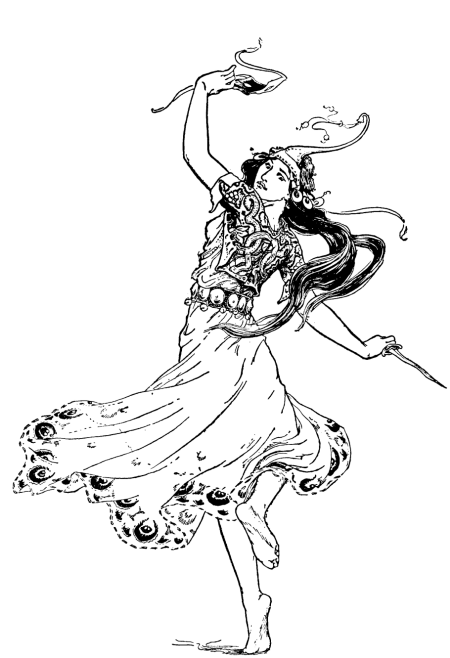
\includegraphics[scale=.5]{Sacraments}
  \end{center}


    \SACRAMENT [
      Name=Bless,
      Link=mystic-sacrament-bless,
      Paradigm=Grace,
      Save=N,
      Duration=Session,
      Counter=None,
      Keywords=Splittable,
      Target=Close Ally or object
    ]

    Choose one unique effect per Grace die invested: 
    1. The Ally can automatically make a single Save roll;
    2. The Ally can automatically succeed on a single \RO or \RS check;
    3. The Ally can immediately end a Markovian duration affecting them;
    4. The Ally or object is Hallowed for the remainder of the Session (this negates the detriment Unhallowed)

    Once an effect is used, it disappears (though the Blessing can be recast)

    \SACRAMENT [
      Name=Consecrate,
      Link=mystic-sacrament-consecrate,
      Paradigm=Grace,
      Save=N,
      Duration=Concentration,
      Counter=None,
      Keywords=None,
      Target=Close radius
    ]

    You exude a \DICE meter diameter circle of \mylink{Hallowed Ground}{miracle-hallowed-ground} around yourself. You cannot move or be carried while concentrating on this Sacrament.

    Note that the area of Hallowed Ground will temporarily cancel out the effects of \mylink{Unhallowed Earth}{occultism-unhallowed-earth} (making it "normal"), but that Sacraments cannot be performed while you are on Unhallowed Earth.

   \SACRAMENT [
      Name=Curse the Unhallowed,
      Link=mystic-sacrament-curse-the-unhallowed,
      Paradigm=Grace,
      Save=Y,
      Duration=0,
      Counter=None,
      Keywords=Splittable,
      Target=\DICE Nearby Unhallowed
    ]


    Up to \DICE Unhallowed creatures take \SUMDICE + \DICE damage (Save for half).  You can divide this damage up any way you like.

    \example {
      Oberlan Xi, Mystic of Pilzesser, performs the sacrament of Curse the Unhallowed on a ghoul and a group of skeletons. He rolls 3 d4 Grace dice in the attempt and gets a 9 - adding the number of \DICE he rolled, this becomes a 12 (9+3).  He can affect up to 3 creatures, and decides to deal 6 damage to the ghoul and 3 damage to two of the skeletons (he could also have just dealt 12 damage to the ghoul if he preferred).
    }  


    \SACRAMENT [
      Name=Heal,
      Link=mystic-sacrament-lay-on-hands,
      Paradigm=Grace,
      Save=N,
      Duration=Concentration,
      Counter=None,
      Keywords=None,
      Target=Close (touch) Allies
    ]

    Heal up to \SUMDICE points of Flesh by touch. You may distribute healing among as many creatures as you would like, as long as the total Flesh healed does not exceed \SUMDICE and you maintain concentration. If you invest 4 \DICE or more, you may instead heal a single target's Flesh fully






   \SACRAMENT [
      Name=Loaves and Fishes,
      Link=mystic-sacrament-loaves-and-fishes,
      Paradigm=Grace,
      Save=N,
      Duration=0,
      Counter=None,
      Keywords=None,
      Target=Close radius
    ]


    You create enough food to feed \SUMDICE people for one meal, along with clean water to fill one mug per person. Mugs, utensils, and condiments are not provided.  Those that participate in the meal do not need to roll Provisions for a Bivouac.  

    \SACRAMENT [
      Name=Meditation,
      Link=mystic-sacrament-meditation,
      Paradigm=Grace,
      Save=N,
      Duration=0,
      Counter=None,
      Keywords=0,
      Target=Self
    ]

    You drop into deep meditation.  It needs to be quiet-ish, so you can't do it during Combat.  You can do up to \DICE of the following (you can only choose each option once per Meditation):
    \mylist {
        \item a) Heal 1 \UD of damage to an Intangible Stat
        \item b) Roll your \FOC and heal that much Flesh (up to \MAX)
        \item c) Roll your \FOC and heal that much Grit (up to \MAX)
        \item d) Purge yourself of a Toxin
    }


    \cbreak


    \SACRAMENT [
      Name=Walk on Water,
      Link=mystic-sacrament-walk-water,
      Paradigm=Grace,
      Save=N,
      Duration=Concentration,
      Counter=None,
      Keywords=Splittable,
      Target=Self and \DICE-1 Close (touch) Allies
    ]

    You and up to \DICE-1 Allies can slowly walk over water for as long as you maintain Concentration. 


  \newpage
    \mysection{Whispers}{arcana-whispers}


    Whispers are the disciplines, incantations, hedge magic, illusion, sleight-of-hand, and minor telepathy that constitute the \mybold{Left Hand Path}.  Passed down through instruction, ancient books, and word-of-mouth, Whispers allow you to trick reality into doing what you want.

    Rolling your \KNAVE should only be required by the Arbiter if the difference between success and failure would be interesting, or when the attempt shouldn't be an automatic success.  Your skill in each of the four Whispers is represented by one of the following \STATIC die, called a \KNAVE.  If you are "Untrained" in one of the Whispers, it means you know only the bare details; you would only succeed if the difference between success and failure would be uninteresting or an automatic success.

    \mytable{X r}{
      \thead{Rank} & \thead{\KNAVE} \\
    }{
      Untrained  & 1 \\
      Apprentice & d4 \STATIC \\
      Footpad & d6 \STATIC \\
      Sharper & d8 \STATIC \\
      Master & d10 \STATIC \\
    }

    You may buy additional ranks in a Whisper when you \mylink{advance in level}{advancement-leveling}

    You must be unarmored or wearing \mylink{Light Armor}{gear-armor} to use your Whispers.  You cannot perform Whispers while using a shield.   Using a Whisper in combat is a \mylink{Basic Maneuver}{combat-basic-maneuver}.  Finally, Whispers require verbalization; you must be able to speak in order to use a Whisper (a common punishment for thieves is to cut out their tongues).

    \example {
        \RB: \KNAVE + Modifiers vs. Target
    } 



    If the Arbiter decides the roll is required, she will set a Target (a number between 2 and 9) for the roll (details on difficulty are found in the Arbiter's section on \mylink{Knavery}{arbiter-knave}).  \RB than this number using your \KNAVE (ties go to the Adventurer!)

    You may use your \LUCK to affect your \KNAVE roll, but it can never provide more than a +4 Modifier.



    \explain {
      Flink Lighthand is 3rd level and a Footpad in the Whispers of Sun Wukong (so he has d6 \KNAVE and d6 \LUCK), and he's robbing a crypt.  Creeping down a hallway he peeks through the broken door of an antechamber, and sees the glint of gold at the far end.  Flink's sixth-sense is tingling though, and he asks the Arbiter if he sees any traps in here.  The Arbiter knows there's a cunning poisoned spear trap in the room and assigns a Target of 4/2 to it (4 to find it and 2 to disarm it).  Flink rolls his \KNAVE and gets a 4 - he smells a whiff of tarantula venom in the air, and the large flagstone just inside the door seems to shimmer for a moment.  Bending close to the flagstone that would release the trap, Flink whispers to it and asks it to lock in place.  He rolls again ... and gets a 1!  Thinking quickly, Flink rolls his \LUCK and rolls a 4.  He adds 4 to his roll, making it a 5.  Lucky break - he mixed up the words of the Whisper, but it worked out better than he hoped. \\~ \\~
     Later, Flink finds himself in a spot where he has to climb a rocky cliff to continue his journey.  Flink is "Untrained" in the Whispers of Anne Bonny, but the Arbiter decides that the difference between success and failure isn't interesting at this point of the adventure (she'd rather get him to the surprises she has on the other side!).  Flink's natural ability as a Knave is enough for him to scamper up the rock face.  If the Arbiter felt that this was difficult enough to not be automatic, Flink could still roll his \LUCK and add it to his rank of 1 (Untrained) to try to get up the wall...

    }

  \begin{center}
  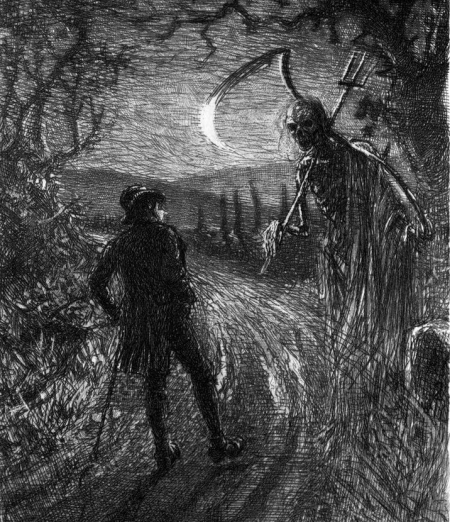
\includegraphics[scale=.5]{Spectre}
  \end{center}




    \mysubsection{Whispers of Anne Bonny}{knave-whisper-ann-bonny}

    Also known as The Swashbuckler, Anne Bonny's instructions show the ways to scale impenetrable fortresses, icy cliffs, and wizard's towers; swing from ropes and vines; disguise yourself to escape patrolling soldiers or to get past armed guards; and forge documents to start wars or gain access to restricted areas. If you are a student of the Whispers of Anne Bonny, a Knave's Sword gains both the Rend and Cleave ability in your capable hands.

    \mysubsection{Whispers of Br'er Rabbit}{knave-whisper-brer-rabbit}

    Br'er Rabbit (The Curious) knows a thing or two about tight squeezes.  His Whispers can help you remove items from pockets without anyone seeing; perform sleight-of-hand, ventriloquism, and distraction to befuddle your marks; escape from ropes and manacles; and cast spells from Fetishes.  If you are a student of the Whispers of Br'er Rabbit, you can turn Invisible (as the spell) once per Session.

    When casting spells from a Fetish, you roll your \KNAVE for the Whispers of Br'er Rabbit instead of Blood Dice.  You can add the result of a \LUCK to this roll as well. The difficulty of reading a spell off a specific Fetish is up to the Arbiter, but the difficulty should default to "automatic"  

    \mysubsection{Whispers of Sun Wukong}{knave-whisper-sun-wukong}

    Sun Wukong is known as The Thief.  His teachings show the secret ways of hiding things on your person so they are difficult to find; uncovering and understanding the mechanisms of traps, snares, and Inscribed Sigils and chide them into disarming themselves; and opening locked chests, doors, and prisons.  If you are a student of the Whispers of Sun Wukong, you can make a sack, bag, or satchel into a Hammerspace Bag.  You can only have 1 Hammerspace Bag in existence at a time.

    \explain {
      The \mybold{Hammerspace Bag} can contain up to 12 Significant Items.  Searching for a Significant Item is a 1-in-(number of items) chance of finding it per Moment i.e. if you have 6 Significant Items in the bag, you have a 1-in-6 chance of pulling it out in a Moment.  You can pull out Insignificant Items stored in the bag immediately.  If you die, all of the contents of the bag are immediately ejected
    }




    \mysubsection{Whispers of The Bride}{knave-whisper-the-bride}

    The Bride is known by many names, none of them spoken aloud:  Lady Death, the Banshee, the Viper, etc.  Education in the Whispers of the Bride teaches you the mental tricks, hypnotism, and observation necessary to sneak past (or behind) people without them noticing you, to silence the clink of coins in your pocket and the sound of your breath and heartbeat. In addition, the Bride teaches you the finer points of committing Murder, provided you get \mylink{the Drop}{combat-surprise} . If you are a student of the Whispers of the Bride, you do not need to make \DEX checks for handling Toxins or Acids.

    \cbreak

    \myhighlight{Murder}{knave-murder}

    If you get \mylink{The Drop}{combat-surprise} on someone, you can attempt a Murder.  Murder can only be performed at Close range with a Shortsword, Dagger, Club, or Hand Axe.  Make a standard Fight \RO; if you hit, pick \mybold{one} of the following attacks:

    \dashedbox {
      \mybullet {
        \item \mybold{Cautious:}  You automatically \mylink{Crit}{combat-crits-and-fumbles} (do maximum damage + \LVL).  Any weapon.
        \item \mybold{Reckless:}  You do 3d6 damage.  Any weapon.
        \item \mybold{Bloody:}  You roll damage normally, but the Monster is also Bleeding. Stabbing only.
        \item \mybold{Waylaying:}  You can either roll damage and the Monster is Woozy, or do no damage and the Monster must Save or be Knocked Out.  Bashing only.
      }
    }

   Murder is a Combat Action, so it can't be combined with other Combat Actions (like Florentine). Damage bypasses any Armor or Soak, if applicable (you slip the blade between the Monster's scales / plate mail / chink in carapace). Once you commit a Murder, you no longer have the Drop unless you're able to get out of sight again. Note that Monsters who are Amorphous or immune to surprise cannot be Murdered. 



  \explain {
    Deego Foxears (3rd Level Knave and student of The Bride) and Stalwart Hamhands (3rd Level Sellsword) come around the corner and surprise a clutch of three Ghouls and a necromancer standing at an altar.  The ghouls are Close and the necromancer is Nearby.  The Arbiter rules the ghouls and necromancer are surprised, so Flink has The Drop.  He tries his Fight \RO and succeeds.  He's armed with a Knave Sword and opts to attack "Cautiously".  He deals 11 damage (8 for the sword + \LVL) and stabs a ghoul through the heart before it can react. Stalwart steps up behind him and guts another ghoul with his polearm.  The single remaining ghoul rolls morale and foolishly decides to stay and fight.

    ~\\

    Deego and Stalwart roll Init - Deego rolls well over 20, Stalwart less so (he's wearing plate mail).  Deego takes the opportunity to duck into the shadows to try to get the Drop on the necromancer. The Arbiter gives the difficulty a 3 (2 for the ghoul's \HD; an extra 1 because the ghoul is Close and aware Deego's there, but he's mostly focused on the huge armored guy with a polearm; and no modifier for the necromancer, who's completely absorbed in his ritual). Deego rolls his d6 and gets a 5, and slips out of view.  The Ghoul attacks Stalwart and hits, but Stalwart is able to absorb the damage with his Grit.  The necromancer seems to be trying to finish his ritual and doesn't make a move.  It's Stalwart and Deego's turn; Deego takes another Tactical Maneuver and moves Nearby (right behind the necromancer), while Stalwart engages the remaining ghoul.  Depending on how Init goes the next Moment, Deego will be able to take a Combat Action, and hopefully stop the wizard from releasing some eldritch horror ...
  }


  \newpage
  \mysection{Wizardry}{arcana-wizardry}

\flavor{[B]lood aids great sorcery!" thundered Xaltotun, in a voice that made the rocks quiver \Tilde R.E.H., "The Hour of the Dragon"}

The arcana of Wizardry are powered through blood; to manifest a spell you must roll one or more of your Blood Dice - how many is up to you, but you have to roll them all at once.  Each Blood Die is a \POOL, meaning if you roll a \myital{natural} 1 or a 2, you lose the die. 

Rolling 3 dice or more carries an additional risk:

\mybullet {
  \item If you roll any triples, roll on the \mylink{Mishap table}{table-mishap}. The spell works.
  \item If you roll any quadruples, roll on the \mylink{Calamity table}{table-calamities}. The spell fails.
  \item If you roll any quintuples, roll on the \mylink{Ruin table}{table-ruin}. The spell fails.  This will most likely kill you.
}

You restore 1 Blood Die when you take a \mylink{Bivouac}{combat-resting-bivouac}.  You restore \myital{all} your Blood Die during a Vacation.  If you are out of Blood, you can attempt to ride \mybold{the Torrent}


\mysubsection{The Torrent}{philosopher-torrent}

If you have 0 Blood Dice in your pool, you can try to cast your Wizardry arcana directly from the Torrent (a dangerous proposition).  For each Blood Die you want to add to your Wizardry, try the following \RO:

\example {
  \mybold{Torrent}

  \RO : \INT plus d6 plus Modifiers ~\\ ~\\

  \myital{Don't forget to add your \LVL, since this roll uses your \INT!}
}

If you succeed, you can add a Blood Die to the spell.  You can do this as many times as you like for each spell. If you fail any \RO attempt, the spell fails and you suffer a \mylink{Calamity}{table-calamities}.

  \begin{center}
  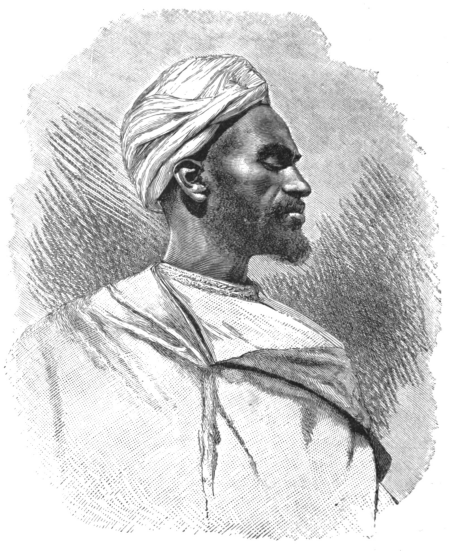
\includegraphics[scale=.5]{Philosopher_1}
  \end{center}


\mysubsection{Components}{philosopher-components}

If you have the \mylink{Virtue: Crux of Blood}{philosopher-virtue-blood}, you can harvest and use components to cast spells:

\example {
  \mybold{Harvest Component}
  \RO : \INT plus d6 plus d20 plus Modifiers

  ~\\
  
  \myital{Don't forget to add your \LVL, since this roll uses your \INT!}
}

If you succeed on your \RO try, gain d4 \UD of a Component.

You decide what Components augment which spells. For example, you could declare that kobold's eyes are a component for the spell Sleep.  If you succeed in your \RO try, then kobold's eyes are always a component for Sleep (note it on your character sheet) for YOU and not for anyone else (someone else's version of Sleep has a different way of casting, needs boggart boogers or whatever). 

If you cast a spell with a Component, then you only burn a Blood die if you roll a 1 (instead of a 1 or 2).  Components are Insignificant items, but using a component consumes it in a puff of smoke / blue flame / swarm of gnats etc.

\mybullet {
  \item Components can only be harvested during a Breather, and have to be from one of the Monsters you've (presumably) killed.  It has to be something you can reasonably carry (Arbiter's choice) - basilisk tongue, OK.  Green slime, not OK.
  \item Monsters only provide one component.  You can't say kobold's eyes help Magic Missile and kobold's tongues help cast Battering Beam.   
  \item You can only try once per Monster type per Breather, so if you kill 9 kobolds and 14 trolls then you get two shots - once on kobolds and once on trolls.
  \item You can only harvest d4 \UD from a Monster no matter how many there are - 9 kobolds or 1, you get d4 \UD
}


\mysubsection{Grimoires}{philosopher-grimoires}

Grimoires are solid, with thick vellum pages and a sturdy cover. Special runes and symbols trap spells inside cages of crystallized thought. Each book contains enough room for 10 spells. Some spells must be stored across several pages for safety, so the books contain more than 10 pages, and have
plenty of room for notes, ledgers, or sketches - and curses, hexes, coded and cryptic entries written with poisonous and hallucinogenic inks. Grimoires start in a waterproof, acid- and fire-resistant bag. Outside the bag, they are not waterproof and are quite flammable. See the section on
\mylink{Inscription}{research-inscription} for more details.


\mysubsection{Fetishes}{philosopher-fetishes}

Fetishes are inscribed with a single spell from your Grimoire, cranium, or another fetish.  All fetishes have a \UD of d4 - when the \UD is exhausted, the magical words disappear from the fetish.  A Sorcerer's skull counts as a fetish, though obviously the brain can't be in the way if you want to read
it.  See the section on \mylink{Inscription}{research-inscription} for more details.

You may cast the spell from the Fetish with any number of Blood you choose, OR you may forgo the Blood die and roll a single d6 for the effect.

\cbreak

\mysubsection{Wizards' Duel}{philosopher-wizards-duel}

Certain spells can be countered by other spells - for example,
\mylink{Balthazar's Breathtaking
Blast}{wizardry-balthazars-breathtaking-blast} can be countered by
\mylink{Mighty Lungs}{wizardry-mighty-lungs}, and
\mylink{Invisibility}{wizardry-invisibility} can be dispelled by the wisps
summoned in the \mylink{Fool's Fire}{wizardry-fools-fire} spell. 

If you attempt to counter a spell and the Sorcerer who cast it is not
present (that is, not somewhere Close, Nearby, Far-Away, or Distant) you
automatically succeed.  Otherwise, you enter into a duel with the other
Sorcerer.

Each Sorcerer must \RB : \INT, adding their \LVL and the \DICE invested in
the spell as well as any other modifiers.  

\example {
  \mybold{A Wizards' Duel is}
  \RB : \INT plus \LVL plus \DICE
}


The winner's spell stays, the loser's spell goes.  Put another way: 

\mybullet{
  \item If you are countering a spell and you win, the spell you're
attempting to counter is dispelled and your spell takes effect
  \item If you are countering a spell and you lose, the spell you're
attempting counter remains and your spell fizzles with no effect.
}

If you attempt to counter a spell and you roll a \mylink{Calamity}{table-calamities} or \mylink{Ruin}{table-ruin}, the counterspell doesn't work. 


\newpage



\SPELL[
  Name=Acid Arrow,
  Link=wizardry-acid-arrow,
  Paradigm=Elements,
  Save=N,
  Duration=0/Markovian,
  Counter=None,
  Keywords=None,
  Target=Nearby or Far-Away Monster or Object
]

You throw an acidic arrow at a Monster or object. You must make a successful Fight check using your \INT (instead of \VIG or \DEX).  If you succeed: 

\mynumlist {
  \item If the target is wearing Armor, they must make a \UD check at the start of every Moment for the Markovian duration of the spell.  If they are using a shield, they may immediately sunder it to nullify the spell; 
  \item If they are not wearing Armor, they must take \DICE additional damage at the start of every Moment for the Markovian duration of the spell; 
  \item If the target is an object, it will melt a \DICE x 10cm cubic area of wood, metal, or stone.  
}

\SPELL[
  Name=Arcadia's Bulwark,
  Link=wizardry-arcadias-bulwark,
  Paradigm=Mind,
  Save=N,
  Duration=Session,
  Counter=\mylink{Acid Arrow}{wizardry-acid-arrow},
  Keywords=None,
  Target=Self
]


A spectral shield with a heraldic device of your choosing appears in the vicinity of your non-dominant arm.  The shield moves on its own to block Throw and Shoot weapons, and can absorb up to \SUMDICE + \DICE damage before it dissipates.  You can also Sunder this shield (like the Combat ability),
which also causes it to dissipate. You can still cast spells while this shield is summoned.  An Acid Arrow fired into the shield will dispel it if a Wizards' Duel is lost.


\SPELL[
  Name=Balthazar's Breathtaking Blast,
  Link=wizardry-balthazars-breathtaking-blast,
  Paradigm=Biomancy,
  Save=Y (negate),
  Duration=Markovian,
  Counter=\mylink{Mighty Lungs}{wizardry-mighty-lungs} ,
  Keywords=None,
  Target=Nearby or Far-Away point
]

A marble-sized bead of shit lands at a Nearby or Far-Away point you select. You can cause the sphere to detonate at any time in \DICE Hours (including immediately). All creatures Close or Nearby the sphere's detonation must
Save or immediately become Sickened, and the area is filled with a thick green mist that lasts for \DICE Hours.  Any who enter the mist during this time must Save or become Sickened, though you smell it and see it before
you're in it, so you won't stumble into it blindly.  Animals will avoid the area for the Markovian duration.  The spell does not affect creatures with no sense of smell, mindless creatures, or creatures who habitually live in
filth (goblins, shambling mounds, etc.).  The mist can be dispelled by Mighty Lungs if a Wizards' Duel is lost.




\SPELL[
  Name=Bastogne's Glamping Charm,
  Link=wizardry-bastognes-glamping-charm,
  Paradigm=Force,
  Save=N,
  Duration=Bivouac,
  Counter=\mylink{Morass}{wizardry-morass} ,
  Keywords=None,
  Target=Close
]



In an area you designate, a magical camp appears where you and \DICE-1 allies can Bivouac. The camp includes a bedroll, a sleeping platform, a small purple and gold tent, a small table and chair, a kettle, a cookpot
with a stew going, an iron arm to hold the kettle or cookpot over a fire, a book entitled "The Erotic Poems of Plumtarch" (less erotic than expected), and a pair of dry wool socks for up to \DICE people. Any items removed from
the area vanish instantly. In the spell's area, the temperature is moderated very slightly, wind and rain are lessened, and vermin cannot enter.  The tents are immune to casual attack, including from wandering Monsters (anyone
sleeping outside the tents might not be so lucky).  Up to \DICE people staying at the camp can forego a single Provisions \UD roll during their Bivouac.  The campsite can be utterly dispelled by Morass if a Wizards' Duel
is lost.

\SPELL[
  Name=Battering Beam,
  Link=wizardry-battering-beam,
  Paradigm=Force,
  Save=N,
  Duration=Concentration,
  Counter=\mylink{Battering Beam}{wizardry-battering-beam},
  Keywords=Contested,
  Target=Close or Nearby Monster or Object
]


A beam of force erupts from your forehead and strikes something you can see, pushing it backwards. Every Moment, the creature or object is pushed 5m in the direction you are looking.  If it's an object, you can push up to \DICE
x100kg.  If it's a creature, they can try to \RB: \VIG with a -\DICE penalty to fight back. If you lose the \RB try, the spell immediately ends - otherwise, the spell lasts as long as you concentrate. 
If the target cannot move backwards, it takes \DICE damage.  The Battering Beam can be dispelled by another Battering Beam if a Wizards' Duel is lost.




\SPELL[
  Name=Cacaphony,
  Link=wizardry-cacaphony,
  Paradigm=Entropy,
  Save=Y (negate),
  Duration=Varies,
  Counter=\mylink{Negasonic Bomb}{wizardry-negasonic-bomb} ,
  Keywords=None,
  Target=Nearby or Far-Away point
]



You roll a small orb of Entropy to a point Nearby or Far-Away; the orb rolls silently and is hard to see.  At any time for the next \SUMDICE Hours, you can have the orb detonate into an incredibly loud clattering, wailing, and
whistling. Creatures Close to the designated point must Save or be Stunned for \DICE Moments. It is audible in clear air up to a \DICE km away. You can designate \DICE conditions under which the orb will detonate. For example,
you could say "now"; "if anyone steps on it"; or "if water touches it".  The conditions must be obvious and must occur within 1m of the orb. When the spell's duration expires, you can choose to have the orb detonate (as above)
or vanish silently.  The Cacaphony can be dispelled by a Negasonic Bomb if a Wizards' Duel is lost.





\SPELL[
  Name=Charm,
  Link=wizardry-charm,
  Paradigm=Mind,
  Save=Y (negate),
  Duration=Session,
  Counter=\mylink{Charm}{wizardry-charm} ,
  Keywords=Contested,
  Target=Close Monster(s)
]



Ensorcel one or more Monsters whose combined \HD is less than or equal to \DICE.  Save negates; otherwise, they will regard you as a good friend and ignore the obvious spell you just cast on them.  The effect lasts for the
entire Session unless you ask them to do something they might think was a little weird: attack an ally, let you through an area they're supposed to be guarding, etc. (this is up to the Arbiter's discretion).  This prompts a
\RB: \FOC try with a -\DICE penalty.  You must touch the target's flesh (like with a handshake) to cast the spell.  The charmed person must stay Close, Nearby, or Far-Away from you - if you ever move beyond this distance, the spell is ended.  
The Charm can be broken and dispelled by another Charm if a Wizards' Duel is lost. 

  \begin{center}
  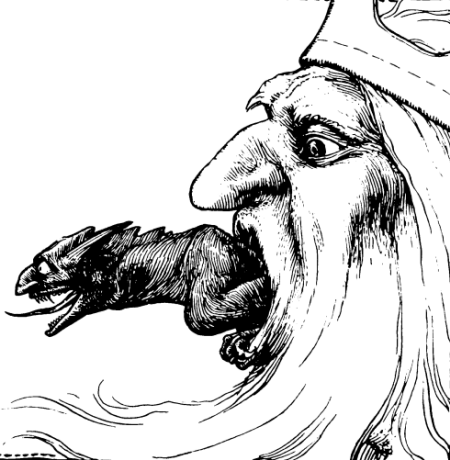
\includegraphics[scale=.5]{Tongue}
  \end{center}


\SPELL[
  Name=Color Spray,
  Link=wizardry-color-spray,
  Paradigm=Mind,
  Save=Y (negate),
  Duration=0 / Markovian,
  Counter=None ,
  Keywords=Splittable,
  Target=Close or Nearby Monster(s)
]



You emit \DICE sprays of color from your fingertips that you can split among \DICE Monsters.  For each Monster, if the \SUMDICE of the \DICE targeting the Monster is twice as much (equal to or greater) as the Monster's \HD, it
is Befuddled (the duration is Markovian and depends on the number of dice invested).  If \SUMDICE is three times the Monster's \HD, it is Stunned for a Moment, then Befuddled as above. If \SUMDICE is five times the creature's
\HD, it is Stunned (the duration is Markovian and depends on the number of dice invested), then Befuddled (Markovian duration).  Save negates.





\SPELL[
  Name=Commanding Presence,
  Link=wizardry-commanding-presence,
  Paradigm=Mind,
  Save=N,
  Duration=Combat or \SUMDICE Minutes,
  Counter=\mylink{Balthazar's Breathtaking Blast}{wizardry-balthazars-breathtaking-blast} ,
  Keywords=None,
  Target=Self
]

You grow +\DICE meters in height, and your features and voice become terrible and commanding.  Creatures of less than \DICE \HD must test morale or flee in terror.  You can use your \INT in place of any rolls where you
would normally use \VIG.  If you enter the radius of Balthazar's Breathtaking Blast, or if the spell is cast Close to you, the Commanding Presence is dispelled if a Wizards' Duel is lost.




\SPELL[
  Name=Ego Weapon,
  Link=wizardry-ego-weapon,
  Paradigm=Mind,
  Save=N,
  Duration=Session,
  Counter=\mylink{Greaseball}{wizardry-greaseball} ,
  Keywords=None,
  Target=Self
]



You can summon a Bashing, Cutting, or Stabbing weapon of Force.  You can change the type of weapon by using 1 Maneuver in Combat.  The weapon does \DICE damage and can hit creatures only affected by magic.  Only you can fight with the Ego Weapon.   You must make a successful
Fight check using your \INT (instead of \VIG or \DEX) to hit with the weapon.  A Helping Hand can wield an Ego Weapon, but you can only have 1 Ego Weapon in existence at a time.  The weapon lasts for the entire Session.  It can be dispelled by a Greaseball if a Wizards' Duel is lost; it will dispel an
Illusion spell with a touch if a Wizards' Duel is won.

\SPELL[
  Name=Enervate,
  Link=wizardry-enervate,
  Paradigm=Entropy,
  Save=Y (half),
  Duration=0,
  Counter=None ,
  Keywords=None,
  Target=Close or Nearby Magical Monster
]




Often used to target sorcerers or seriously magical creatures (unicorns, dragons, etc).  In the case of Philosophers who know the Crux of Blood, they take \DICE damage for each
unspent Blood pool they possess; in the case of a magical Monster, they take \SUMDICE+\DICE damage.  Save for half damage, but Philosophers who fail their Save
must also immediately roll their remaining Blood die as if they were casting a spell (any rolls of a 1 or a 2 loses the die; if you roll doubles a Mishap occurs; etc) though no spell will actually be cast.   Non-magical creatures,
or creatures that have no Blood die, are unaffected by this spell.



\SPELL[
  Name=Fireball,
  Link=wizardry-fireball,
  Paradigm=Elements,
  Save=Y (half),
  Duration=0,
  Counter=None ,
  Keywords=None,
  Target=Any point
]

Throw a ball of fire somewhere Close, Nearby, or Far Away.  Everyone Close
to the detonation takes \SUMDICE fire damage (Save for half), and highly
flammable things are set aflame (curtains, dry trees, and oil but not people
or buildings).




\SPELL[
  Name=Fogbank,
  Link=wizardry-fogbank,
  Paradigm=Elements,
  Save=N,
  Duration=Combat or \SUMDICE Minutes,
  Counter=\mylink{Mighty Lungs}{wizardry-mighty-lungs} ,
  Keywords=None,
  Target=Close
]



You summon a bank of swirling and shifting fog that exists for as long as
you concentrate.  The fog can move with you, or you can mentally direct it
to move Nearby (takes 1 Maneuver).  The fog will blanket \SUMDICE creatures
or a space \DICE+\DICE meters cubed.  Missiles that are thrown or shot into
the fog strike a random target; nothing can be thrown or shot out of the
fog.  The fog extinguishes small flames (torches, candles, etc)  Creatures
who attempt to Fight while inside of the fog act as if they were Befuddled;
however, anyone attempting to Murder someone else in the fog
succeeds automatically.



  \begin{center}
  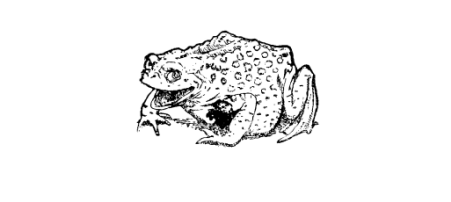
\includegraphics[scale=.5]{Toad}
  \end{center}



\SPELL[
  Name=Fool's Fire,
  Link=wizardry-fools-fire,
  Paradigm=Entropy,
  Save=Y (negate),
  Duration=Concentration,
  Counter=\mylink{Enervate}{wizardry-enervate} ,
  Keywords=Splittable,
  Target=Close or Nearby point
]



You project \DICE will-o'the-wisps into an area Close or Nearby.  The wisps
can move one range (Close to Nearby, Nearby to Far Away, etc) each Moment
for as long as you concentrate.  You can split the wisps up any way you like
but they can't be more than Far-Away from you.  The wisps do not shed heat,
do not require air, and can't be doused by water.  They shed a steady yellow
light the brightness of a torch.  At the top of the Moment, you can command
up to \DICE wisps to Befuddle up to \DICE Monsters that are Close to them.  The Befuddle affect lasts as long as you concentrate. 
The Monsters immediately get a Save to negate (one for each wisp that's targeting them), but a successful Save does not end the spell.  
If any of the wisps are struck by an Enervate spell, they are all dispelled if a Wizards' Duel is lost.  When a wisp is dispelled, any Monsters
Befuddled by the wisp are released from the effect.



\SPELL[
  Name=Greaseball,
  Link=wizardry-greaseball,
  Paradigm=Entropy,
  Save=N,
  Duration=Markovian,
  Counter=\mylink{Pritchard's Gusty Belch}{wizardry-pritchards-gusty-belch} (acid) ,
  Keywords=None,
  Target=Close or Nearby Monster or Object
]



Toss a small ball of grease at a point on the ground Close or Nearby. If you
would prefer to throw the ball at a person or object, make a Fight \RO using
your \INT - if you miss, it dissipates.  If thrown at the ground, the
surface becomes slick with a thick oil; anyone attempting to move through
the area must \RO using \DEX+\MD with a -\DICE penalty or immediately fall
Prone.  It requires a successful \RO as above to get up again.  If you throw it at a
creature, the effect is as above, plus they can't hold anything without
dropping it.  If you throw it at an object, the object becomes impossible to
carry or hold until the grease is removed with a mild or strong acid. 
Pritchard's Gusty Belch (acid variety) will dispel the grease if a Wizards'
Duel is lost.  The grease is highly flammable.  





\SPELL[
  Name=Grimm's Electric Fingers,
  Link=wizardry-grimms-electric-fingers,
  Paradigm=Elements,
  Save=Y (half),
  Duration=0,
  Counter=None ,
  Keywords=None,
  Target=Close or Nearby Monster or Object
]



Forks of lightning erupt from your outstretched hands, striking a Close or
Nearby target for \SUMDICE damage (Save for half). You can cause the
lightning to "jump" up to \DICE-1 times to another creature or object Close
by, provided they are conductive (iron armor, metal ladders, etc).  Magic
swords aren't conductive.  You can "ping-pong" between two objects if you
desire. Creatures struck by any bolt after the first take \DICE damage
(no Save). Objects struck by subordinate bolts will become
momentarily electrified, and deal a shock that could cause someone to lose
their grip unless they \RO : \VIG + \FOC with a -\DICE penalty.



\SPELL[
  Name=Hammerspace Mule,
  Link=wizardry-hammerspace-mule,
  Paradigm=Force,
  Save=N,
  Duration=Session,
  Counter=\mylink{Illusion}{wizardry-illusion} ,
  Keywords=Hammerspace,
  Target=Close
]



You create a spectral mule out of pure Force. The mule carries two
magical saddlebags that can each hold \SUMDICE Significant Items whose
combined weight doesn't exceed \DICE x 200kg (a reminder that a person is 25
Significant Items, and small creatures are 15).  The mule walks at a brisk
trot.  It will stop and turn at your verbal command, but you cannot make it
reverse or slow down. You can only give it the commands "go", "stop",
"left", and "right". If the mule takes any damage, it immediately disappears
and drops all the items on the ground.  The mule will obey your last command
until the spell's duration expires.  Hammerspace Mules think that Illusions
are real; if the Illusion would damage them in some way (a pit they would
fall into, a spear they would run into, etc) the Mule is dispelled (dropping
its items on the ground) if a Wizards' Duel is lost.





\SPELL[
  Name=Helping Hand,
  Link=wizardry-helping-hand,
  Paradigm=Biomancy,
  Save=N,
  Duration=Concentration,
  Counter=\mylink{Web}{wizardry-web} ,
  Keywords=None,
  Target=Self
]



You can detach either hand from its wrist.  The
hand floats at chest height and can hold anything you could normally hold. 
The hand can't use any weapons except for an Ego Weapon.  It can grab
shirts, press buttons, and shove people (but not too hard).  If anyone
attacks the hand, you have to roll your Guard as if they were attacking you. 
If your hand takes any damage, it disappears for the rest of the Session. 
Additionally, if the Hand is ever caught in a Web spell, it will disappear
if a Wizards' Duel is lost.  At the end of the Session, roll a d6.  If you roll a 1, your hand comes back 
as something else (a claw, a tentacle, etc) at the Arbiter's discretion - 
otherwise, it returns as normal.



\SPELL[
  Name=Heroic Leap,
  Link=wizardry-heroic-leap,
  Paradigm=Biomancy,
  Save=N,
  Duration=0,
  Counter=None ,
  Keywords=None,
  Target=Self or Close Ally
]



You and up to \DICE-1 allies can leap \VIG+\SUMDICE meters high and/or
\VIG+\SUMDICE meters forward in a straight line.  You take no damage on
landing, provided you land on or above the level you started from. For
example, you could leap from the ground to top of a steeple, or you could
leap over the steeple to land on the ground, but you couldn't leap from the
top of a steeple to the ground.  When you land, you can make a \RS : \DEX
(\RS : \INT if you are the caster) and if you succeed,
you can leap again. You can do this up to \DICE times.  You can't cast
spells or Fight while you're jumping around.





\SPELL[
  Name=Hollow Head,
  Link=wizardry-hollow-head,
  Paradigm=Biomancy,
  Save=N,
  Duration=Session,
  Counter=None ,
  Keywords=Hammerspace,
  Target=Self
]



You brain disappears and your head has a hinge that opens like a box, but
only you know this and only you can open it. For the rest of the Session,
you are immune to the next \DICE spells from the Mind paradigm, and you can
fit up to \SUMDICE Significant Items inside of your head in Hammerspace
(pulling one of these items out takes a Maneuver).  When you resist the
final Mind paradigm spell, the enchantment immediately ends. If the spell
ends while items are stored in your head they will mix with your
brain-matter. Usually this is fatal, though ambitious sorcerers sometimes
add drugs.  While your head is hollow, another sorcerer could read the
spell(s) inscribed on the inside.


  \begin{center}
  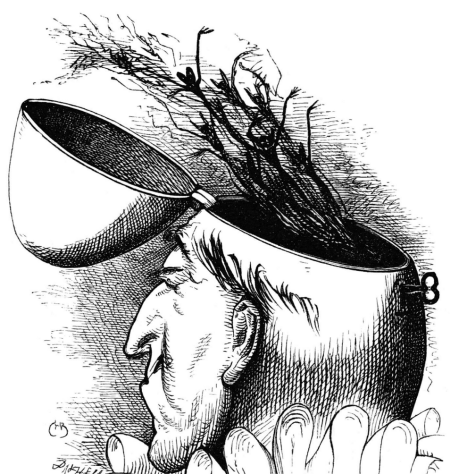
\includegraphics[scale=.5]{HollowHead}
  \end{center}





\SPELL[
  Name=Ice Bridge Step,
  Link=wizardry-ice-bridge-step,
  Paradigm=Elements,
  Save=N,
  Duration=Session,
  Counter=\mylink{Greaseball}{wizardry-greaseball} ,
  Keywords=None,
  Target=Self
]



You and up to \DICE-1 allies can run over liquids as if they were land.  Ice
forms beneath your feet with each step. If you slow down (to walk, fight,
etc), you'll sink. Very wavy seas may require you to \RS : \DEX.  Very hot
liquids (like lava) may require you to \RS : \INT.  The ability is dispelled
if you are struck by a Greaseball spell and you fail a Wizards' Duel.





\SPELL[
  Name=Icebolt,
  Link=wizardry-icebolt,
  Paradigm=Elements,
  Save=Y (half),
  Duration=0 / Markovian,
  Counter=None ,
  Keywords=None,
  Target=Close or Nearby point (straight line)
]



Throw a bolt of ice at a target Close or Nearby.  The bolt will travel in a
straight line from your fingers.  Anything touched by the bolt takes
\SUMDICE damage, Save for half.  Additionally, everything that fails its
Save is frozen to whatever surfaces they are touching.  Keys are frozen in
locks; swords are frozen to hands; boots are frozen to the ground
(creatures are usually immobilized from the boots down unless they were
playing in a fountain or something).  The objects are stuck until the
for a Markovian duration, based on the number of \DICE used.




\SPELL[
  Name=Illusion,
  Link=wizardry-illusion,
  Paradigm=Mind,
  Save=N,
  Duration=Varies,
  Counter=\mylink{Ego Weapon}{wizardry-ego-weapon} ,
  Keywords=None,
  Target=Varies
]



You create an illusion of anything you desire. If anything touches the
illusion, it will pass through it with no effect.  The illusion cannot be
greater than \DICE x \DICE meters in size.  Think of the illusion as a
perfectly accurate hologram that you are creating - the illusion can be
heard in addition to being seen, can perform the same action over and over
again, and can deliver messages, but it can't interact in a meaningful way
or perform complex actions based on external forces. 

Each aspect of the illusion requires one or more Blood die to cast:

\mylist {
  \item You want the illusion to say up to \DICE + \DICE words or make \DICE
+ \DICE sounds (wailing, shouting, etc)
  \item You want the illusion to be a physical thing (hole in the ground,
stone wall, orc guard, etc)
  \item You want the illusion to be able to move up to \DICE meters
  \item You want to cast the illusion on a living creature (disguise them as
a beggar or a lamp post)
}

Note that there is some Arbiter's discretion here.  A guard pacing in front
of a door might cost 2 \DICE (a physical thing moving back and forth 2
meters), but if you want the illusion of acrobats or pouncing lions it will
be more costly.  A disguise cast on someone to appear to be a beggar might
cost 1 [die] (a living creature wearing the face and clothing of a random
beggar), but disguising yourself as the king will be significantly harder.

The Illusion will last for \DICE Hours.  Anyone touching the illusion will
immediately know it to be fake, but this doesn't cause the illusion to
disappear.  However, if the illusion is touched with an Ego Weapon, it will
disappear if a Wizards' Duel is lost.





\SPELL[
  Name=Invisibility,
  Link=wizardry-invisibility,
  Paradigm=Entropy,
  Save=N,
  Duration=Varies,
  Counter=\mylink{Fool's Fire}{wizardry-fools-fire} ,
  Keywords=None,
  Target=Self or Close Allies or Objects
]



Up to \DICE objects or creatures can be made invisible (including yourself),
and will remain that way as long as they don't move.  As soon as the
creature or object moves (or is moved), the charm is broken.  Invisible
creatures can see other invisible and hidden objects (including Knaves using Whispers).  If this spell is cast on something Invisible, it will force the
object to become seen.  The duration of the charm depends on the dice
invested.  1 [die]: \SUMDICE Moments; 2 \DICE: Minutes; 3 \DICE: Hours; 4
\DICE Days; 5 \DICE: Weeks; 6+ \DICE: Forever.  The wisps from a Fool's Fire
can dispel the Invisibility of a Wizards' Duel is lost.

  \begin{center}
  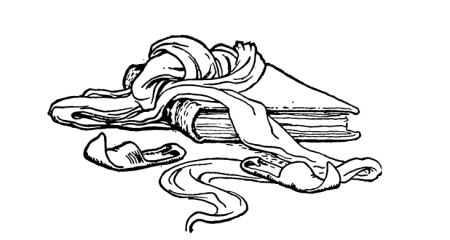
\includegraphics[scale=.5]{Invisibility}
  \end{center}





\SPELL[
  Name=Kelsier's Swarm of Irritating Vermin,
  Link=wizardry-kelsiers-swarm-of-irritating-vermin,
  Paradigm=Force,
  Save=N,
  Duration=Markovian,
  Counter=\mylink{Mighty Lungs}{wizardry-mighty-lungs} ,
  Keywords=None,
  Target=Close; Nearby; Far Away
]



You summon a cloud of tiny, magical, irritating vermin to an area Close,
Nearby, or Far-Away.  The vermin deal \DICE damage per Moment to every
living creature Close to them, but no damage to nonliving creatures or
objects. At the top of each Moment they are in the cloud, a non-mindless
creature must Save or take a -\DICE penalty on their Fight roll.  The vermin
won't move from the spot where they are summoned, and will remain until the
spell expires.  If the target is an object, the vermin will do minor
cosmetic damage, such as chewing holes in paper, gnawing wood, chipping
paint, and scratching glass.  Mighty Lungs will dispel the swarm if a
Wizards' Duel is lost.



\SPELL[
  Name=Knife Trick,
  Link=wizardry-knife-trick,
  Paradigm=Force,
  Save=N,
  Duration=Session,
  Counter=\mylink{Grimm's Electric Fingers}{wizardry-grimms-electric-fingers} ,
  Keywords=Splittable,
  Target=Close; Nearby; Far Away
]



Up to \DICE daggers orbit your head like a halo or crown.  These must be
daggers in your possession.  Magic and silver daggers are OK, as are other
"dagger-like" items (icicles, shards of glass, etc) at the Arbiter's
discretion.  At any time during the Session, you can mentally "throw" one or
more of these daggers at things that are Close, Nearby, or Far-Away with
unerring accuracy.  This could be used to sever a rope or pin something to a
wall (or stick into someone's chest) - but no Gambits, that wouldn't be
fair.  Each dagger does \SUMDICE+\DICE damage i.e. if you were to throw 1
dagger at someone, it would do d6+1, two daggers 2d6+2, etc.  Grimm's
Electric Fingers will dispel the magic and cause the daggers to fall to the
ground if a Wizards' Duel is lost.





\SPELL[
  Name=Knock,
  Link=wizardry-knock,
  Paradigm=Entropy,
  Save=N,
  Duration=0,
  Counter=\mylink{Lock}{wizardry-lock} ,
  Keywords=None,
  Target=Close or Nearby Objects
]



\DICE Close or Nearby object(s) is/are opened. Doors are flung wide, locks
are broken, shackles are bent open, belts come undone.  Ideas or thoughts
can be unlocked from a mind if a \RB : \INT contest is lost. Objects locked
by the Lock spell are opened if a Wizards' Duel is won.




\SPELL[
  Name=Levitating Disc,
  Link=wizardry-levitating-disc,
  Paradigm=Force,
  Save=N,
  Duration=Concentration,
  Counter=\mylink{Suspend Objects}{wizardry-suspend-objects} ,
  Keywords=None,
  Target=Close or Nearby point in space
]



You draw a circle in the air of \DICE+\DICE diameter, in any orientation. The inside of the
circle is made of Force, as solid as iron. You can cause the circle to
raise, lower, or hover in place.  You can only move up and down (never
side-to-side).  Up to \DICE people could stand under it and be completely
covered, or on it and be levitated provided they don't weigh more than \DICE
x200kg.  If you lower the circle on top of someone, they take \DICE damage
per Moment. The circle moves 10 meters a minute (about 3m per Moment).  You can change the disc's orientation
at any time.  If the Levitating Disc is targeted with Suspend Objects, the
disc will be dispelled if a Wizards' Duel is lost.





\SPELL[
  Name=Lipby Chonk's Viscous Form,
  Link=wizardry-lipby-chonks-viscous-form,
  Paradigm=Biomancy,
  Save=N,
  Duration=Combat or \SUMDICE Minutes,
  Counter=None ,
  Keywords=None,
  Target=Self
]



Your flesh becomes gelatinous. You can squeeze through gaps as small as a 
keyhole with a great deal of effort. You take no damage from Crushing
attacks for the duration of the spell. The spell only affects your flesh,
not anything you're wearing or carrying.




\SPELL[
  Name=Lock,
  Link=wizardry-lock,
  Paradigm=Mind,
  Save=Y (negate),
  Duration=Markovian,
  Counter=None ,
  Keywords=None,
  Target=Close and Nearby Objects
]



Up to \DICE non-living thing slam shut and can't be opened. If the object is
a door, chest, or something like it, it will slam shut forcefully and
loudly. This spell can work on things that aren't portals (a sword could be
locked in its scabbard). You can also use this spell to lock a specific
memory or thought, making it immune to mind reading or scrying without a \RB
: \INT try.  The duration is Markovian and depends on the number of
\DICE invested.  The Lock can be dispelled by the Knock spell if a Wizards'
Duel is lost.


\SPELL[
  Name=Meat Shield,
  Link=wizardry-meat-shield,
  Paradigm=Biomancy,
  Save=N,
  Duration=Combat or \SUMDICE Minutes ,
  Counter=None ,
  Keywords=None,
  Target=Close and Nearby
]

You summon a giant slab of meat.  The meat has \SUMDICE+\DICE Health, and
can fill an area \DICE meters cubed.  The meat weighs \DICE x100kg and lasts
for \DICE Hours.  Zoological creatures will attack the Meat Shield first. 
Up to \DICE other creatures can eat the Meat Shield in lieu of rolling their
Provisions, but the provenance of the meat is ... unknown.  If a Scything
Disc of Nog is used on a Meat Shield, the shield will be dispelled if a
Wizards' Duel is lost (otherwise, it will take damage as normal).





\SPELL[
  Name=Mighty Lungs,
  Link=wizardry-mighty-lungs,
  Paradigm=Biomancy,
  Save=N,
  Duration=Until exhalation,
  Counter=None ,
  Keywords=Contested,
  Target=Self
]

Your next inhalation allows you inhale 10x the normal amount of air. Not
only does this allow you to hold your breath for 10x as long, but if you
exhale forcefully it will release a blast of air strong enough to knock
pigeons out of air and polish your teeth. A human-sized creature is knocked
Prone and pushed Nearby unless they try a \RB: \DEX or \VIG
(their choice) with a -\DICE penalty vs your \INT.  This spell will also blow open all
closed but unlocked doors in a room, shatter all windows in a
building, or knock the thatched roof off a peasant's shack. If you cast this
spell with 3 or more \DICE, Save or your teeth shatter.




\SPELL[
  Name=Mirror Image,
  Link=wizardry-mirror-image,
  Paradigm=Entropy,
  Save=N,
  Duration=Combat or \SUMDICE Minutes,
  Counter=None ,
  Keywords=None,
  Target=Self
]



You create \DICE illusory images of yourself, which move as you move and
always stay Close to you. They are constantly stepping through each other,
so that it is impossible to tell which is which. When an enemy attacks you,
they'll always hit an image first.  An image vanishes as soon as it suffers
a solid impact (a blow from a mace, but also a slap). Area effects such as a
dragon's breath will cause all images to instantly vanish (and you take the
damage, naturally).





\SPELL[
  Name=Morass,
  Link=wizardry-morass,
  Paradigm=Elements,
  Save=N,
  Duration=Concentration,
  Counter=\mylink{Bastogne's Glamping Charm}{wizardry-bastognes-glamping-charm} ,
  Keywords=Contested,
  Target=Nearby or Far-Away Area
]



The ground \SUMDICE meters in radius and \DICE meters deep turns to black
muck.  Monsters and objects in the mud sink 1 meter per Moment.  At the top of
the Moment, a creature can \RB: \VIG with a -\DICE penalty vs. your \INT 
to pull themselves out 1 meter (if they were only 1 meter deep to
begin with, they escape).  If someone's head dips below the mud (2m for
people, 1m for Pooka, 4m or more for giants), they immediately being drowning and must make a \DEATH 
roll at the top of every Moment they are submerged (they can still claw their way up 1m with a successful \RB try,
as above).  If they don't have a \DEATH, they die in \HD Moments.

The spell lasts for as long as you concentrate.  When you break your
concentration, everything that sunk in the mud is immediately vomited back to
the surface.   If the area covered by the Morass is targeted by Bastogne's
Glamping Charm, the Morass will be dispelled (and the objects brought to the
surface) if a Wizards' Duel is lost.




\SPELL[
  Name=Negasonic Bomb,
  Link=wizardry-negasonic-bomb,
  Paradigm=Mind,
  Save=N,
  Duration=Concentration,
  Counter=\mylink{Cacaphony}{wizardry-cacaphony} ,
  Keywords=None,
  Target=Nearby or Far Away Area
]



You roll a small orb of Mind to a point Close, Nearby or Far-Away; the orb
rolls silently and is hard to see.  When the orb stops rolling it
immediately and silently detonates.  Creatures Close to the designated point
are Deafened until they leave the area of effect.  Likewise, no spells can
be cast while Close to the Negasonic Bomb.  Murder attempts against anyone deafened in this way succeed automatically. The spell lasts as long as
you concentrate.  The bomb can be dispelled by Cacaphony if a Wizards' Duel
is lost.





\SPELL[
  Name=Prismatic Ray,
  Link=wizardry-prismatic-ray,
  Paradigm=Entropy,
  Save=Y (half),
  Duration=0,
  Counter=None ,
  Keywords=Splittable,
  Target=Nearby or Far-Away
]



A brilliant white light emanates from your forehead to a point Nearby or
Far-Away, where it splits into a prism of \DICE beams.  Each beam strikes a
random Ally or Monster Close to the prism.  Roll a d8 on the table below for
each beam and apply its results.

\mynumlist {
  \item \mybold{Red} Target takes \DICE fire damage, Save for half. Highly flammable things catch fire.
  \item \mybold{Orange}  Target takes \DICE bashing damage, Save for half. 
  \item \mybold{Yellow} Target takes \DICE lightning damage, Save for half.  If you fail your Save, you drop what you're holding.
  \item \mybold{Green} Target takes \DICE acid damage, Save for half. Roll your Armor \UD if applicable.
  \item \mybold{Blue} Target takes \DICE ice damage, Save for half. If you fail your Save, you fall Prone.
  \item \mybold{Indigo} Target takes \DICE stabbing damage, Save for half.
  \item \mybold{Violet} Target takes \DICE chopping damage, Save for half.
  \item \mybold{Roll} again.  Instead of \DICE damage, the effect deals \SUMDICE damage.. If you get this result again, the beam splits and the target takes an additional effect (roll again and apply the result).  Continue in this way until you don't roll an 8.
}





\SPELL[
  Name=Pritchard's Gusty Belch,
  Link=wizardry-pritchards-gusty-belch,
  Paradigm=Biomancy,
  Save=N,
  Duration=0,
  Counter=None ,
  Keywords=None,
  Target=Close and Nearby Area
]



You can breathe out up to \DICE elements (fire, acid, water, wind, steam, etc)
immediately in front of you for a Moment.  The elements don't interact with
one another and act independently, so if you were to belch out fire and
water, you would get the effects of both.  If the order matters (set
something on fire and immediately douse it with water), you pick the order
of effects.  Water breath is enough to extinguish fires smaller than a big
bonfire, or wash off acid; wind breath could push a small sailboat or blow
swarming insects out of an area; acid breath bleaches the color from objects
and irritates the eyes; fire breath would cause paper and flammable objects
(but not people, unless they were doused in oil) to catch fire, etc.




\SPELL[
  Name=Protection from Element,
  Link=wizardry-protection-from-element,
  Paradigm=Elements,
  Save=N,
  Duration=Session,
  Counter=\mylink{Prismatic Ray}{wizardry-prismatic-ray} ,
  Keywords=Splittable,
  Target=Self or Close Allies
]



Reduce all damage of a single chosen element (acid, cold, fire, lightning,
etc) by -\DICE.  The spell protects its targets from the negative effects of
the natural elements (desert heat, arctic chill) as well.  If you are struck
by a Prismatic Ray of the same elemental type, the protection is dispelled
if a Wizards' Duel is lost.


  \begin{center}
  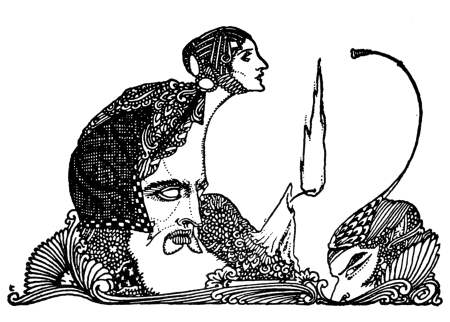
\includegraphics[scale=.5]{Wizardry_1}
  \end{center}



\SPELL[
  Name=Rhea's Efficacious Plow,
  Link=wizardry-rheas-efficacious-plow,
  Paradigm=Force,
  Save=N,
  Duration=Moments,
  Counter=None ,
  Keywords=None,
  Target=See description
]



You send an invisible wedge of Force along the ground in a straight line up
to a Distant point.  The wedge can take up to \DICE turns ("left" or
"right") at your command.  Any light debris on the path (snow, small stones,
leaves, grass) is pushed to the side; fields can be tilled. Any pressure
plates or tripwires are activated. You do not have to be able to see the
entire path, but you do need to know the approximate route the wedge will
take. The wedge can't move through solid objects, and it can't hurt anyone (though it will push them to the side).
The path cleared is \DICE meters wide. If you cast this spell with 3 \DICE
or more, the width becomes \SUMDICE meters wide.




\SPELL[
  Name=Sandstorm,
  Link=wizardry-sandstorm,
  Paradigm=Elements,
  Save=N,
  Duration=Concentration,
  Counter=None ,
  Keywords=None,
  Target=Close
]



You cough up a swirling spiral of sand.  Small flying creatures (bug-sized),
arrows, and spears cannot enter or leave the sandstorm.  Up to \DICE-1 other
people can hide in the sandstorm with you.  The sand moves with you and
lasts as long as you concentrate.



\SPELL[
  Name=Sanguine Mail,
  Link=wizardry-sanguine-mail,
  Paradigm=Biomancy,
  Save=N,
  Duration=Session,
  Counter=\mylink{Enervate}{wizardry-enervate} ,
  Keywords=None,
  Target=Self
]



You become encased in elaborate plate mail that seems to be made from
constantly congealing blood.  You definitely stand out in a crowd. Your \MD
drops to d4, but you can still cast spells.  The \UD for the Armor depends
on the number of \DICE invested: 1 d3; 2 d4; 3 d6; 4 d8; 5 d10; 6+ d12.  If
you are struck with an Enervate spell, the Sanguine Mail is dispelled if a
Wizards' Duel is lost.





\SPELL[
  Name=Scuttle,
  Link=wizardry-scuttle,
  Paradigm=Biomancy,
  Save=N,
  Duration=Combat or \SUMDICE Minutes,
  Counter=\mylink{Greaseball}{wizardry-greaseball} ,
  Keywords=None,
  Target=Self
]



Your clothes and hair animate to carry you around. You can move at full
speed in any orientation, and you can freely rotate as you move. For
instance, you could run while standing on your head, holding a torch, and
turning counterclockwise. You can lie on your side and, while flipping end
over end, move backwards. This effect does not allow you to climb up walls,
but ladders and ropes are no problem (you could suspend yourself from a rope
and cast spells, for example).  If you are struck with a Greaseball, or
attempt to climb something affected by Greaseball, the Scuttle is dispelled
if a Wizards' Duel is lost.




\SPELL[
  Name=Scything Disc of Nog,
  Link=wizardry-scything-disc-of-nog,
  Paradigm=Force,
  Save=Y (half),
  Duration=0,
  Counter=None ,
  Keywords=None,
  Target=Nearby or Far Away Area
]



You hurl a whirling disc of Force and light from your fingertip. The disc
screeches like a sawblade. It deals \SUMDICE damage to its target, Save for
half. If it deals more than 6 damage, it bounces towards a random creature
(friend, foe, or even yourself) Close or Nearby, dealing \SUMDICE-2
damage, Save for half. If it deals more than 6 damage, it bounces towards
another random creature Close or Nearby, dealing \SUMDICE-4 damage, Save for
half. This continues, losing 2 damage with each bounce, until there are no
valid targets or the spell deals 6 or less damage to a creature.





\SPELL[
  Name=Sleep,
  Link=wizardry-sleep,
  Paradigm=Mind,
  Save=Y (negate),
  Duration=Markovian,
  Counter=\mylink{Cacaphony}{wizardry-cacaphony} ,
  Keywords=None,
  Target=Close or Nearby Area
]



You summon a cloud of somnolent dust to a point Close or Nearby. 
\SUMDICE creatures Close to the cloud, who have no more than \DICE \HD, must
immediately Save or fall into a magical slumber.   They can't be awakened by
anything less than a vigorous slap (counts as a Maneuver).  You don't have
control over who falls asleep, it's entirely random and will be as many
creatures as possible (up to \SUMDICE).  You are immune to your own Sleep
spell (so you could cast it Close to yourself).  Creatures who fall asleep
immediately fall Prone and drop any items they're holding.  Fight rolls
against them will hit automatically and do maximum damage, and can only be
blocked by Armor.  This will wake the creature up, of course.  If an orb of
Cacaphony is detonated Nearby, the creatures will awaken if a Wizards' Duel
is lost.  Otherwise, creatures who fall asleep will remain asleep for the
Markovian duration.   




\SPELL[
  Name=Summon Candles,
  Link=wizardry-summon-candles,
  Paradigm=Force,
  Save=N,
  Duration=Varies,
  Counter=\mylink{Fogbank}{wizardry-fogbank} ,
  Keywords=None,
  Target=Close
]



\SUMDICE dribbling candles appear on objects you touch. You can walk around
placing candles as required for Minutes. The candles are lit and burn for
Hours. They can be detached, but will fade from existence within Minutes. 
For every 6 candles placed Close to one another, the wizard close to the
candles gains 1 of the following (your choice): Safe Casting: Replace one of
your rolled Blood Die with a natural 1; Power Casting: Replace one of your
rolled Blood Die with a natural 6; Natural Casting: add a natural +1 to any
Blood Die you've rolled.  When you use 1 of these powers, the 6
candles immediately disappear.  Note that \myital{any} sorcerer can use these
abilities, friend or foe.  A philosopher will immediately know if they are in
an area of candles, and what powers it can bestow on them.  If the candles
are encased in a Fogbank, they are snuffed out and dispelled if a Wizards'
Duel is lost.





\SPELL[
  Name=Suspend Objects,
  Link=wizardry-suspend-objects,
  Paradigm=Force,
  Save=Y (negate),
  Duration=Concentration,
  Counter=\mylink{Levitating Disc}{wizardry-levitating-disc} ,
  Keywords=None,
  Target=Any Distance
]



You can hold up to \DICE objects in the air, weighing no more than \DICE
x200kg.  You can allow these objects to descend at 3m per Moment at your
discretion. Creatures who are brought to ground in this way take no falling
damage.  Unwilling creatures (flying Monsters, for example) get a Save to
negate.  If a Levitating Disc is summoned in the midst of the held
creatures, the Suspend Objects spell will be dispelled (and the objects will
fall) if a Wizards' Duel is lost.




\SPELL[
  Name=Tempestuous Chariot,
  Link=wizardry-tempestuous-chariot,
  Paradigm=Elements,
  Save=N,
  Duration=One trip,
  Counter=None ,
  Keywords=None,
  Target=Close
]



A tumult of air elementals lifts you and \DICE-1 others and takes you in any
direction the you desire, up to \SUMDICE km away.   One catch - the
elementals can only travel in a straight line, and you have to choose
beforehand the way to go ("up", "east", "that way", etc).  While you are in
the tempest you are buffeted horribly and can neither talk nor act.  The
winds refuse to travel without you, and will immediately dispel if you lose
contact




\SPELL[
  Name=Vertigo,
  Link=wizardry-vertigo,
  Paradigm=Mind,
  Save=Y (negate),
  Duration=Markovian,
  Counter=\mylink{Suspend Objects}{wizardry-suspend-objects} ,
  Keywords=None,
  Target= Any Distance
]



You can cause up to \DICE Close, Nearby, Far-Away, or Distant creatures to
suffer severe vertigo unless they Save.  Creatures that are climbing or
flying immediately fall; creatures who are Close to the edge of something (a
cliff, a wall, the guardrails of a ship, etc) need to \RS : \FOC or fall.
Creatures already on the ground will fall Prone.  If the creatures are
struck with a Suspend Objects spell, the Vertigo is dispelled if a Wizards'
Duel is lost.




  \begin{center}
  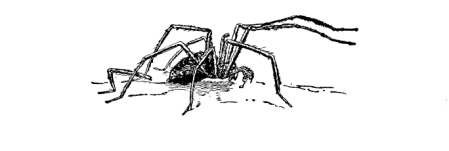
\includegraphics[scale=.5]{Spider}
  \end{center}


\SPELL[
  Name=Web,
  Link=wizardry-web,
  Paradigm=Entropy,
  Save=Y (negate),
  Duration=Markovian,
  Counter=None ,
  Keywords=None,
  Target=Nearby or Far Away Area
]



You can anchor a giant web between three or more solid points up to \DICE
meters in radius (for example: the 4 points of a door, two trees and the
ground, across a hallway, etc).  Objects that touch the web immediately
become stuck; arrows and spears can't be fired through it.  Creatures that
enter the web (or are caught in it when cast) must Save or become ensnared
for the Markovian duration (each creature should roll their Markovian die
separately). Fight rolls against them hit automatically and can only be
blocked by Armor.  The web is extremely flammable and will be consumed in
\DICE Moments.



\SPELL[
  Name=Whirling Blades,
  Link=wizardry-whirling-blades,
  Paradigm=Entropy,
  Save=N,
  Duration=Concentration,
  Counter=\mylink{Suspend Objects}{wizardry-suspend-objects} ,
  Keywords=None,
  Target=Self
]



You summon a number of invisible blades of Force that spin around your
waist, with you in the center.  Every creature Close to you takes \DICE
damage for each Moment the spell is maintained.  The blades will cut or
damage fragile objects.  If the creature or object sits above or below your
waist, they take no effect.  If the blades are struck by a Suspend Objects
spell, they will be dispelled if a Wizards' Duel is lost.




  \newpage

  
}%end

